\documentclass[twoside]{report}
\usepackage{../estilo-apuntes}

%\usepackage[utf8]{inputenc}
%\usepackage[T1]{fontenc}
%\usepackage[francais]{babel}
%\usepackage{lmodern}

%\usepackage{epstopdefi}

%\usepackage[spanish]{babel}
%\usepackage[T1]{fontenc}


%\usepackage[latin1]{inputenc}


\title{\textsc{Resumen de la asignatura\\ Geometría Aplicada.}}
\author{\textsc{Ismael Ruiz Donaire}\\ \textsc{Mercedes Prado Rodríguez}\\ \textsc{Jesús Rebollo Bueno}}
\date{}



\usepackage{makeidx}
\makeindex

%\newtheorem{thm}{Teorema}

%\theoremstyle{definition}
%\newtheorem{defi}[thm]{Definición}
%\newtheorem{nt}[thm]{Nota}
%\newtheorem{obs}[thm]{Observación}
%\newtheorem{ej}[thm]{Ejemplos}


%\theoremstyle{Teorema}
%\newtheorem{propo}[thm]{Proposición}
%\newtheorem{coro}[thm]{Corolario}
%\newtheorem{lema}[thm]{Lema}
%\newtheorem{lemaa}[thm]{Lema A}
%\newtheorem{lemab}[thm]{Lema B}
%\newtheorem{lemac}[thm]{Lema C}

\newcommand{\rojo}[1]{\textcolor{red}{#1}}
\newcommand{\azul}[1]{\textcolor{blue}{#1}}
\newcommand{\verde}[1]{\textcolor{green}{#1}}
\newcommand{\amarillo}[1]{\textcolor{yellow}{#1}}
\newcommand{\celeste}[1]{\textcolor{cyan}{#1}}
\newcommand{\magenta}[1]{\textcolor{magenta}{#1}}
\def\dx{\,{\rm d}x}
\newcommand{\fracc}[2]{{\displaystyle\frac{#1}{#2}}}
\newcommand{\ul}[1]{\underline{#1}}
\newcommand{\bs}[1]{\boldsymbol{#1}}
\newcommand{\colocapdf}[2]{\quad\pdfimage width #2 {pdfs/#1.pdf}}


\begin{document}


\maketitle{}




\chapter{Aplicaciones entre Superficies}

Vamos a introducir las definciones, enunciados de teoremas y ejemplos, con el fin de poder usar este documento en el examen de la asignatura.

\begin{defi}[función diferenciable]\label{1}
Sea $M$ una superficie regular (sup.reg.) en $\mathbb{R}^3$. Una $\textbf{función}$ continua $f: M \rightarrow \mathbb{R}$ se dice $\textbf{diferenciable}$ en un punto $p \in M$ si existe una superficie simple $(U,\textbf{x})$ en $M$ tal que  $p \in U$ y $ f\circ \textbf{x}$ es diferenciable en $p' = \textbf{x}^{-1}(p)$. f será diferenciable en $M$ si lo es en todo punto de $M$.
\end{defi}

\begin{prop}
La \textup{\textbf{Definición \ref{1}}} no depende de la supeficie simple tomada.
\end{prop}
\begin{dem}
Sean M una superficie una superficie regular y $f:M\to\R$ una aplicación continua, $p\in M$ y $(U,\X)$ una superficie simple tal que $p \in \X(U)$ y satisface las condiciones de la Definición \ref{1}. Sea otra superficie simple $(V,\Y)$ en las condiciones anteriores. Como $(U,\X)$ y $(V,\Y)$ son superficies simples de una misma superficie regular, deben ser compatibles en la intersección. Es decir, podemos considerar la aplicación diferenciable $\X^{-1}\circ \Y \func{\Y^{-1}(W)}{X^{-1}(W)}$, donde $W=\X(U)\cap\X(V)$. Consideramos:
\[
f\circ \Y = (f \circ \X)\circ (\X^{-1}\circ \Y)
\]
Como todas las aplicaciones son diferenciables, deducimos que $f\circ \Y$ también lo es en $p''=\Y^{-1}(p)$. 

\QED
\end{dem}

\begin{prop}\label{3}
Sean $f: \mathbb{R}^3 \rightarrow \mathbb{R}$ una función diferenciable y $M$ una sup.reg. en $\mathbb{R}^3$. Entonces $f\vert_M : M \rightarrow \mathbb{R}$ es diferenciable.
\end{prop}
\begin{dem} Sea $f\func{\R^3}{\R}$ una aplicación diferenciable. Sea M una superficie regular en $\R^3$. Tenemos que $f$ es continua en $\R^3$, de donde se deduce que $f|_M$ es continua. En efecto, sea $I\subset \R$ abierto, $f^{-1}|_M(I)\cap M = f^{-1}(I)\cap M  \subset M$ abierto relativo, por lo que es continua. Sea $p\in M$. Veamos que $f|_M$ es diferenciable en $p$. Sea $(U,\X)$ una s.s. de M en $p$. Entones $f|_M \circ \X = f \circ \X$, puesto que $X(U)\subset M$. Por tanto, $f\circ \X$ es diferenciable en $U$ y $p'\in U \subset \R^2$ abierto.\QED
\end{dem}

\begin{nota}
La \textbf{Proposición \ref{3}} vale también si tomamos $f: G \subseteq \mathbb{R}^3 \rightarrow \mathbb{R}$ con $G$ abierto y $M\subseteq G$.
\end{nota}

\newpage

\begin{ejs}\
\begin{enumerate}
\item \textbf{Distancia a un punto (al cuadrado).}


Sean $p_0=(x_0,y_0,z_0)$ un punto de $\mathbb{R}^3$ y $f: \mathbb{R}^3 \rightarrow \mathbb{R}$ tal que $f(x,y,z)=(x-x_0)^2+(y-y_0)^2+(z-z_0)
^2$. Entonces $f\vert_M$ es diferenciable con $M$ sup.reg. de $\mathbb{R}^3$.

\item \textbf{Distancia a un punto. }

Sean $p_0=(x_0,y_0,z_0)$ un punto de $\mathbb{R}^3$
y $f: \mathbb{R}^3 \setminus\lbrace p_0\rbrace \rightarrow \mathbb{R}$ tal que $f(x,y,z)=\sqrt{(x-x_0)^2+(y-y_0)^2+(z-z_0)
^2}$. Entonces  $f\vert_M$ es diferenciable con $M$ sup.reg. de $\mathbb{R}^3$ tal que $p_0 \notin M$.

\item \textbf{Función altura sobre un plano  $\pi_0$.}

Sean $\pi_0$ un plano de $\mathbb{R}^3$ que pasa por $p_0=(x_0,y_0,z_0)$, con vector característico unitario $\overrightarrow{v}=(a,b,c)$, y $f: \mathbb{R}^3 \rightarrow \mathbb{R}$ tal que $f(q)=(q-p_0)\overrightarrow{v}$ (distancia signada a $\pi_0$). Así, $f(x,y,z)=a(x-x_0)+b(y-y_0)+c(z-z_0)$. Entonces, si $M$ es sup.reg. de $\mathbb{R}^3$, $f\vert_M$ es diferenciable.
\end{enumerate}
\end{ejs}

\begin{defi}
Una aplicación $f: M \rightarrow \mathbb{R}^n$ es \textbf{diferenciable} si $\pi_i \circ f: M \rightarrow \mathbb{R}$ es diferenciable $\forall i =1,...,n$, siendo $\pi_i : \mathbb{R}^n \rightarrow \mathbb{R}$ la proyección i-ésima.
\end{defi}

\begin{defi}\label{7}
Sean $M$,$N$ sup.reg. y $f: M\rightarrow N$ una aplicación continua. Se dice que $f$ es \textbf{diferenciable} en $p\in M$  si existen $(U,\textbf{x})$ en $M$ con $p \in \textbf{x}(U)$ y $(V,\textbf{y})$ en $N$ con $f(p) \in \textbf{y}(V)$ tales que $\textbf{y}^{-1}\circ f \circ \textbf{x}$ es diferenciable en $p' = \textbf{x}^{-1}(p)$.
\end{defi}


\begin{nota}
$f$ es diferenciable en $M$ si $f$ es diferenciable en $p$, $\forall p \in M$.
\end{nota}

\begin{prop}
La \textup{\textbf{Definición \ref{7}}} no depende de las superficies simples.
\end{prop}
\begin{dem}
Sea $p\in M$, $(U_1,\X_1)$ tal que $p\in\X_1(U_1)$ y $(V_1,\Y_1)$ tal que $f(p)\in\Y(V_1)$ satisfaciendo las condiciones de la definición 7. Sean  $(U_2,\X_2)$ y $(V_2,\Y_2)$ cumpliendo las mismas condiciones. Como las cartas son compatibles en sus respectivas superficies, podemos considerar las aplicaciones diferenciables $\Y_2^{-1}\circ \Y_1$ y $\X_1^{-1}\circ \X_2$. Por tanto, $$\Y_2^{-1}\circ f\circ \X_2=(\Y_2^{-1}\circ \Y_1)\circ (\Y_1^{-1}\circ f\circ\X)\circ(\X_1^{-1}\circ \X_2).$$
Así pues, $\Y_2^{-1}\circ f\circ \X_2$ es diferenciable en $p''=\X_2^{-1}(p)$ por ser composición de diferenciables.\QED
\end{dem}



\begin{teorema}
Sean  $f: \mathbb{R}^3 \rightarrow \mathbb{R}^3$ diferenciable, $M$,$N$ sup.reg. tales que $f(M) \subseteq N$. Entonces $f\vert_M : M \rightarrow N$ es también diferenciable.(Se puede cambiar $f: G \subseteq \mathbb{R}^3 \rightarrow \mathbb{R}^3$ con $G$ abierto y $M\subseteq G$).
\end{teorema}

\begin{dem} Sea $f\func{\R^3}{\R^3}$ una aplicación diferenciable, entonces, en particular, es continua. Sean $M$ y $N$ dos superficies regulares en $\R^3$ con $f(M)=N$. Veamos que $f|_M\func{M}{N}$ es continua. Sea $H\subset N$ abierto, $\exists J\subset \R^3$ abierto tal que $G=J\cap N$. Entonces $f|_M^{-1}(H) = f^{-1}(H)\cap M = f^{-1}(J\cap N)\cap M=f^{-1}(J)\cap f^{-1}(N)\cap M = f^{-1}(J)\cap M$ abierto relativo en M, puesto que $F^{-1}(J)\subset \R^3$ es abierto. Luego, $f|_M$ es continua.

Sea $p\in M$. Veamos que $f|_M\func{M}{N}$ es diferenciable en $p$. Sea $(U,\X)$ una s.s. de M en $p\in\X(U)$ y $(V,\Y)$ un s.s. en N con $f(p)\in\Y(V)$. Consideramos la composición en $\Y^{-1}\circ f \circ \X$, que tiene sentido en $\X^{-1}(W)$, donde $W = f^{-1}(\Y(V))\cap \X(U)$. Además, se tiene que $\Y^{-1}\circ f \circ \X = \Y^{-1}\circ f|_M \circ \X$ en $\X^{-1}(W)$ y es diferenciable por ser composición de funciones diferenciable en $p'=\X^{-1}(p)$. Por tanto $f|_M$ es diferenciable.\QED
\end{dem}

\begin{ej}

\

\begin{enumerate}
\item
Si $M$ es \textbf{superficie simétrica respecto del plano $XY$}, entonces $f: M \rightarrow M$ tal que $f(x,y,z)=(x,y,-z)$ es diferenciable, por ser restricción de $\widehat{f} : \mathbb{R}^3 \rightarrow \mathbb{R}^3$ ($M$ = catenoide, $S^2$, cilindro,...).

\item Si $M$ es de \textbf{revolución respecto del eje $OZ$}, la rotación de ángulo $\theta$ respecto a Z, $f_{\theta}: M\rightarrow M$, es diferenciable, por ser restricción de $f_{\theta}: \mathbb{R}^3 \rightarrow \mathbb{R}^3$, dada por $f(x,y,z)=(x\cos\theta - y\sin\theta, x\sin\theta+ y\cos\theta,z)$.

\item
Como $f: \mathbb{R}^3 \rightarrow \mathbb{R}^3:(x,y,z)\longmapsto(ax,by,cz)$ con $a$,$b$,$c >0$ ctes, es diferenciable, entonces su restricción a $S^2$, $f\vert_{S^2}: S^2 \rightarrow E$, también es diferenciable, siendo $E$ el elipsoide de semiejes $a,b,c$.

\item
Como $f: \mathbb{R}^3 \rightarrow \mathbb{R}^3$, $f(p)= Ap + T$, con $A$ matriz ortogonal y $T$ traslación, es diferenciable, entonces $f\vert_{M}: M \rightarrow f(M)$ también lo es.

\item \textbf{Aplicación antipodal.}
$f: \mathbb{R}^3 \rightarrow \mathbb{R}^3:(x,y,z) \longmapsto (-x,-y,-z)$ es diferenciable. Entonces $f\vert_{S^2}: S^2 \rightarrow S^2$ también lo es. (Es un caso particular del ejemplo 4, tomando $A= -$Id, $T=0$, es decir, la \textbf{simetría central respecto del origen}).
\end{enumerate}
\end{ej}


\begin{defi}
Una aplicación $f: M\rightarrow N$ se dice \textbf{regular} en $p\in M$ si existen $(U,\textbf{x})$ en $M$ con $p \in \textbf{x}(U)$ y $(V,\textbf{y})$ en $N$ con $f(p) \in \textbf{y}(V)$ tales que $\textbf{y}^{-1}\circ f \circ \textbf{x}$ es regular en $p' = \textbf{x}^{-1}(p)$, i.e., $J_{p'}(\textbf{y}^{-1}\circ f \circ \textbf{x})$ es una matriz regular.
\end{defi}

\begin{nota}
La \textup{\textbf{Definición 12}} no depende de las superficies simples.
\end{nota}

\begin{defi}
Sean $M,N$ superficies regulares. Una aplicación $f:M\to N$ se llama \textbf{difeomorfismo} si es biyectiva, diferenciable y de inversa diferenciable.
\end{defi}

\begin{nota}
$f$ biyectiva y regular $\Leftrightarrow$ $f$ difeomorfismo.
\end{nota}

\section{La Diferencial o Aplicación Tangente}

\begin{defi}
Dados $f:M \to N$ diferenciable y $p\in M$, se define la \textbf{diferencial de $f$ en $p$} como la aplicación $f_{*p}: T_p (M)\rightarrow T_{f(p)}(N)$ dada por $f_{*p}\overrightarrow{v}=(f\circ\gamma)'(0)$, $\forall \overrightarrow{v}\in T_p(M)$, siendo $\gamma:(-\varepsilon,\varepsilon)\to M$ una curva diferenciable tal que $\gamma(0)=p$ y $\gamma'(0)=\overrightarrow{v}$.
\end{defi}


\begin{teorema}
Sean $f:M\rightarrow N$ diferenciable y $p\in M$.
\begin{itemize}

\item [a)]
$f_{*p}: T_p (M)\rightarrow T_{f(p)}(N)$ no depende de la curva tomada, es lineal y ``su" matriz es $J_{p'}(\textbf{y}^{-1}\circ f \circ \textbf{x})$, con $p'= \textbf{x}^{-1}(p)$.
\item [b)]
Si $f$ es regular en $p$, entonces $f_{*p}$ es un isomorfismo (aplicación lineal y biyectiva).
\end{itemize}
\end{teorema}
\begin{dem}
Sean $M$ y $N$ dos superficies regulares y sea $f:M\to N$ una aplicación diferenciable. Sea $p\in M$ y $\vec{v}\in T_p(M)$. Sean $(U,\X)$ y $(V,\Y)$ dos superficies simples en $M$ y $N$ respectivamente, con $p\in\X(U)$ y $f(p)\in\Y(V)$. Sea $\gamma:(-\varepsilon,\varepsilon)\to M$ una curva diferenciale en $M$ con $\gamma(0)=p$ y $\gamma'(0)=\vec{v}$. Podemos suponer WLOG que $\gamma(t)\in\X(U)\ \forall t\in(-\varepsilon,\varepsilon)$ y que $f\circ\gamma(t)\in\Y(V)\ \forall t\in(-\varepsilon,\varepsilon)$.  

Como $p\in\X(U)\Rightarrow p=\X(u_0^1,u_0^2)$, donde $u^1,u^2$ son los parámetros de la superficie simple $(U,\X)$. Como $\gamma$ es una curva diferenciable en $M$ y $\gamma(t)\in\X(U)\ \forall t\in(-\varepsilon,\varepsilon)$, entonces existen aplicaciones $u^1(t),u^2(t)$ tales que $\gamma(t)=\X(u^1(t),u^2(t))\ \forall t\in(-\varepsilon,\varepsilon)$. En particular, $p=\gamma(0)=\X(u^1(0),u^2(0))$, luego por la inyectividad de $\X$ deducimos que $u^1_0=u^1(0)$ y $u^2_0=u^2(0)$.  

Por otro lado $\vec{v}\in T_p(M)$ y $\{\X_1(u^1_0,u^2_0),\X_2(u^1_0, u^2_0)\}$ es una base de ese espacio, luego existen $\lambda^1,\lambda^2$ tales que 
$$\vec{v}=\lambda^1\X_1(u^1_0,u^2_0)+\lambda^2\X_2(u^1_0,u^2_0),$$
donde $\X_i(u^1_0,u^2_0)=\frac{\partial\X}{\partial u^i}|_{(u^1_0,u^2_0)}$. Tenemos $\vec{v}=\gamma'(0)$ y $\gamma(t)=\X(u^1(t),u^2(t))$, así que derivamos.
$$\vec{v}=\frac{\partial\X}{\partial u^1}|_{(u^1(0),u^2(0))}\frac{du^1}{dt}|_{t=0}+\frac{\partial\X}{\partial u^2}|_{(u^1(0),u^2(0))}\frac{du^2}{dt}|_{t=0}$$
Por tanto, como vimos antes que $u^1_0=u^1(0)$ y $u^2_0=u^2(0)$, $\lambda^i= \frac{du^i}{dt}|_{t=0}$. 

Ahora, $f(p)=f(\gamma(0))=f(\X(u^1_0,u^2_0)$ y $f(p)\in\Y(V)\Rightarrow\exists v^1_0, v^2_0\mid f(p)=\Y(v^1_0,v^2_0)$. Entonces $f\circ\gamma$ es una curva diferenciable en $N$ y $(f\circ\gamma)(t)\in\Y(V)\ \forall t\in(-\varepsilon,\varepsilon)$. Luego exsten aplicaciones $v^1(t),v^2(t)$ tales que $(f\circ\gamma)(t)=\Y(v^1(t),v^2(t))\ \forall t\in(-\varepsilon,\varepsilon)$. En particular, $(f\circ\gamma)(0)=f(p)=\Y(v^1_0,v^2_0)$, por lo que $v^1(0)=v^1_0$ y $v^2(0)=v^2_0$. Entonces, aplicando la regla de la cadena y sustituyendo $t=0$
$$f_{*p}\vec{v}=(f\circ\gamma)'(0)=\sum_{i=1}^2\frac{\partial\Y}{\partial v^i}|_{(v^1(0),v^2(0))}\frac{dv^i}{dt}|_{t=0}=\sum_{i=1}^2\Y_i(v^1_0,v^2_0)\frac{dv^i}{dt}|_{t=0}.$$
Por tanto, $f_{*p}\vec{v}\in T_{f(p)}(N)$ y $\{\Y_1(v^1_0,v^2_0),\Y_2(v^1_0,v^2_0)\}$ es una base de dicho espacio. Por ello existen $\mu^1,\mu^2$ tales que $$f_{*p}\vec{v}=\mu^1\Y_1(v^1_0,v^2_0)+\mu^2\Y_2(v^1_0,v^2_0).$$
Por lo anterior, sabemos que de hecho $\mu^1=\frac{dv^1}{dt}|_{t=0}$ y $\mu^2=\frac{dv^2}{dt}|_{t=0}$.

Como $f$ es diferenciable en $p$, la aplicación $\Y^{-1}\circ f\circ\X$ es diferenciable en un entorno abierto $\overline{U}$ de $p'=(u^1_0,u^2_0)$. Dado $(u^1,u^2)\in\overline{U}$, $\Y^{-1}\circ f\circ\X(u^1,u^2)=(v^1,v^2)=(v^1(u^1,u^2),v^2(u^1,u^2))$, por lo que

$$J_{p'}(\Y^{-1}\circ f\circ\X)=\begin{pmatrix}
\frac{\partial v^1}{\partial u^1} & \frac{\partial v^1}{\partial u^2}\\
\frac{\partial v^2}{\partial u^1} & \frac{\partial v^2}{\partial u^2}
\end{pmatrix}$$

Teniendo en cuenta las expresiones de $\lambda^i$ y $\mu^i$ podemos sustituir y encontrar
$$\mu^i=\frac{fv^i}{dt}|_{t=0}=\sum_{j=1}^2\frac{\partial v^i}{\partial v^j}|_{p'}\frac{du^j}{dt}|_{t=0}=\sum_{j=1}^2\frac{\partial v^i}{\partial u^j}|_{p'}\lambda^j$$
En conclusión, $f_{*p}$ es una aplicación lineal entre $T_p(M)$ y $T_{f(p)}(N)$, y la matriz de dicha aplicación respecto de las bases $\{\X_1(u^1_0,u^2_0),\X_2(u^1_0, u^2_0)\}$ y $\{\Y_1(v^1_0,v^2_0),\Y_2(v^1_0,v^2_0)\}$ es $J_{p'}(\Y^{-1}\circ f\circ\X)$. Además, la expresión para $f_{*p}\vec{v}$ es independiente de la curva diferenciable tomada. Con esto hemos demostrado la primera parte del teorema.

Para la segunda parte basta recordar que si la matriz de la aplicación lineal es regular, entonces la aplicación es biyectiva (por tanto isomorfismo). \QED

\end{dem}

\begin{ej}
Aplicación antipodal en $S^2$, es decir $f:S^2\to S^2$ definida por $f(x,y,z)=(-x,-y,-z)$. Ya vimos que $f$ es diferenciable. Sea $p\in S^2$ un punto fijado. Veamos cómo se define $f_{*p}$. Supongamos que $p$ está en el hemisferio norte de la esfera. Consideramos las superficies simples en $S^2$ siguientes:
$$\X:U\subseteq\R^2\to\R^3\mid \X(u^1,u^2)=(u^1,u^2,\sqrt{1-(u^1)^2+(u^2)^2})$$ 
$$\Y:U\subseteq\R^2\to\R^3\mid \Y(u^1,u^2)=(u^1,u^2,-\sqrt{1-(u^1)^2+(u^2)^2}$$
Los abiertos serían $U=V=\{(x,y)\in\R^2\mid x^2+y^1<1\}$. Como ejercicio probar que efectivamente son superficies simples. Nos quedaría sin cubrir el ecuador.

Tomamos $(u^1,u^2)\in U$. Entonces $$\Y^{-1}\circ f\circ \X(u^1,u^2)=\Y^{-1}\circ f(u^1,u^2,\sqrt{1-(u^1)^2+(u^2)^2})=\Y^{-1}(-u^1,-u^2,\sqrt{1-(u^1)^2+(u^2)^2})=(-u^1,-u^2).$$
Por tanto $\Y^{-1}\circ f\circ \X:U\to V$ tal que $(u^1,u^2)\mapsto (-u^1,-u^2)=(v^1,v^2)$, por lo que su matriz jacobiana sería
$J_{p'}(\Y^{-1}\circ f\circ \X)=\begin{pmatrix}
\frac{\partial v^1}{u^1}	& \frac{\partial v^1}{u^2}\\
\frac{\partial v^2}{u^1}	& \frac{\partial v^1}{u^2}
\end{pmatrix}=\begin{pmatrix}
-1	& 0\\
0	& -1
\end{pmatrix}=-Id,$ con $p'=\X^{-1}(p)$. Por tanto $f_{*p}:T_p(S^2)\to T_{-p}(S^2)$ está definida como $\vec{v}\mapsto -\vec{v}$.
\end{ej}

\section{Isometrías}

\begin{defi}
 Dadas $M$,$N$ sup.reg., una aplicación diferenciable $f:M \longrightarrow N$ se dice \textbf{isometría} si $f$ es biyectiva, regular y  $f_{*p}$ es isometía $\forall p \in M$.
\end{defi}


\begin{nota}

\

\begin{enumerate}
\item \textbf{Toda isometría es difeomorfismo}.

\item
Que $f_{*p}: T_p (M)\rightarrow T_{f(p)}(N)$ sea isometría quiere decir que $$I_p (\overrightarrow{v_1},\overrightarrow{v_2}) = I_{f(p)}(f_{*p}\overrightarrow{v_1},f_{*p}\overrightarrow{v_2}),$$ $\forall p \in M$, $\forall \overrightarrow{v_1},\overrightarrow{v_2} \in T_p(M)$, siendo $I_p$ (resp. $I_{f(p)}$) la Primera Forma Fundamental en $p$ (resp. $f(p)$).
\item \textbf{Las isometrías conservan las longitudes de las curvas}.
\end{enumerate}

Cada una de las definiciones de isometría son para sustituir la parte ``$f_{*p}$ es isometría''.

\begin{proof}
Si $f_{*p}$ es isometría $\forall p\in M$, por definición $f$ conserva las longitudes de las curvas $\Leftrightarrow$ dada $\alpha:(-\varepsilon,\varepsilon)\to M$ una curva diferenciable y dados $t_0,t_1\in (-\varepsilon,\varepsilon)$ con $t_0<t_1$, se tiene que $L_{t_0}^{t_1}(\alpha)=\int_{t_0}^{t_1}||\alpha'(t)||dt$. Por tanto $ L_{t_0}^{t_1}(\alpha)=L_{t_0}^{t_1}(f\circ\alpha)\Leftrightarrow\int_{t_0}^{t_1}||\alpha'(t)||dt=\int_{t_0}^{t_1}||(f \circ\alpha)'(t)||dt\Leftrightarrow ||\alpha'(t)||=||(f\circ\alpha)'(t)||\ \forall t\in (-\varepsilon,\varepsilon)$. Recordemos que en esencia, la primera forma fundamental es el producto escalar, luego si se conserva el módulo se conserva la primera forma fundamental y recíprocamente.

Vamos a ver que $2$ implica $3$. Sea $\alpha$ una curva diferenciable en $M$ y sea $t_0\in(-\varepsilon,\varepsilon)$. Sea $p=\alpha(t_0)$ y consideramos la aplicación tangente a $M$ en $p$, $f_{*p}$. Dado $\vec{v}=\alpha'(t_0)$, $f_{*p}\vec{v}=(f\circ\alpha)'(t_0)$. Por hipótesis, tenemos que $I_p(\vec{v},\vec{v})=I_{f(p)}(f_{*p}\vec{v},f_{*p}\vec{v})$. Esto es equivalente a $||\vec{v}||^2=||f_{*p}\vec{v}||^2$, luego hemos obtenido la condición $3$ tal como la habíamos descrito en el párrafo anterior.

Otra posible definición sería: la aplicacón $f$ verifica $\forall p\in M$ que $||\vec{v}||=||f_{*p}\vec{v}||\ \forall\vec{v}\in T_p(M)$. Esta será la definición que más usaremos. Veamos que esta definición implica $2$.  Sean $\vec{v}_1,\vec{v}_2\in T_p(M)$. Por simetría y bilinealidad, 
$$I_p(\vec{v}_1+\vec{v}_2,\vec{v}_1+\vec{v}_2)=I_p(\vec{v}_1,\vec{v}_1)+I_p(\vec{v}_2,\vec{v}_2)+2I_p(\vec{v}_1,\vec{v}_2)$$
Despejando
$$2I_p(\vec{v}_1,\vec{v}_2)=||\vec{v}_1+\vec{v}_2||^2-||\vec{v}_1||^2-||\vec{v}_2||^2$$
y también se tiene
$$2I_p(f_{*p}\vec{v}_1,f_{*p}\vec{v}_2)=||f_{*p}\vec{v}_1+f_{*p}\vec{v}_2||^2-||f_{*p}\vec{v}_1||^2-||f_{*p}\vec{v}_2||^2$$
Como por hipótesis se tiene la igualdad de módulos se deduce el resultado.
\end{proof}
\end{nota}


\begin{defi}
Se dice que $M$ es \textbf{localmente isométrica}
 a $N$ si $\forall p \in M$, existen $U'$ entorno abierto de $p$ en $M$, $V'$ abierto en $N$ y $f: U' \rightarrow V'$ isometría. Si $M$ es localmente isométrica a $N$ y $N$ es localmente isométrica a $M$, se dice que son localmente isométricas.
\end{defi}


\begin{ej}
El catenoide y el helicoide \textbf{completos} son localmente isométricos, pero \textbf{NO} isométricos, pues no son homeomorfos (el catenoide no es simplemente conexo y el helicoide sí lo es).
\end{ej}
\begin{proof}
Tenemos una parametrización del catenoide $M$ dada por 
\[ \X : U = (0,2\pi) \times (\sinh^{-1}(-1),\sinh^{-1}(1)) \to M \]
\[ \X(u,θ) = (\cosh u \cos θ, \cosh u \sin θ, u) \]
y la parametrización del helicoide $N$ dada por:
\[ \Y : V = (0,2\pi) \times (-1,1) \to N \]
\[ \Y(v,φ) = (v\cos φ, v \sin φ, φ) \]

Dado $p \in M$ tomamos $U' \subset M$ y $V' \subset N$ abiertos tal que $U'=\X(U)$ y $V'=\Y(V)$. Sea $f$ definida para todo $q \in U'$ dada por $f(q)=f(\X(u,θ))=\Y(\sinh u, θ) \in V'$.
Se tiene que $f$ es biyectiva y regular (compruébalo). Veamos que $f_{*q}$ es isometría para todo $q \in U'$. Veamos que, dado $q \in U'$, $f_{*q}$ conseva los módulos de los vectores de $T_q(M)$. Sea $w \in T_q(M)$, entonces existen $λ¹$ y $λ²$ tales que $w=λ¹\X_1(u_0,θ_0)+λ²\X_2(u_0,θ_0)$ donde $q=\X(u_0,θ_0)$.

Tenemos que $f_{*q}(w) \in T_{f(q)}(N)$ dada por $f_{*q}(w) = μ¹\Y_1(v_0,φ_0)+μ² \Y_2(v_0,φ_0)$, donde $f(q)=\Y(v_0,φ_0)=(f\circ \X)(u_0,θ_0)$, luego $v_0 = \sinh u_0$ y $φ_0=θ_0$. Entonces:
\[ \begin{pmatrix}μ¹\\μ²\end{pmatrix} = J_{q} (\Y^{-1} \circ f \circ \X) \begin{pmatrix}λ¹\\λ²\end{pmatrix} = \begin{pmatrix}\cosh u_0 & 0\\0 & 1\end{pmatrix} \begin{pmatrix}λ¹\\λ²\end{pmatrix} = \begin{pmatrix}λ¹ \cosh u_0\\ λ²\end{pmatrix}\]

Calculamos los coeficientes métricos (se omiten los cálculos):

Para $M$:
\[ g_{11} = (\sinh u)^2+1 \]
\[ g_{12} = g_{21} = 0 \]
\[ g_{22} = (\cosh u)^2 \]
Para $N$:
\[ h_{11} = 1 \]
\[ h_{12} = h_{21} = 0 \]
\[ h_{22} = v^2+1 \]

Entonces:
\begin{align*}
	||w||^2 & = I_q(w,w) = (λ¹)^2g_{11}(u_0,θ_0)+(λ²)^2g_{22}(u_0,θ_0)+2λ¹λ²g_{12}(u_0,θ_0) = \\
	& = (λ¹)^2 ((\sinh u_0)+1) + (λ²)^2(\cosh u_0)^2 = (λ¹)^2 (\cosh u_0)^2 + (λ²)^2(\cosh u_0)^2
\end{align*}
\begin{align*}
	||f_{*q}(w)||^2 & = I_{f(q)} (f_{*q}(w),f_{*q}(w)) = (μ¹)^2 h_{11}(v_0,φ_0)+(μ²)^2h_{22}(v_0,φ_0) + 2μ¹μ² h_{12}(v_0,φ_0) = \\
	& = (λ¹)^2(\cosh u_0)^2 + (λ²)^2((\sinh u_0)^2+1) = (λ¹)^2 (\cosh u_0)^2 + (λ²)^2(\cosh u_0)^2
\end{align*}
Luego $||f_{*q}(w)||^2 = ||w||^2$ $\forall w$ y $f$ es una isometría.
\end{proof}

\begin{figure}[!ht]
  \centering
    \includegraphics[width=0.5\textwidth]{HelicoidCatenoid}
\end{figure}\

\begin{teorema}[\textbf{Caracterización de superficies localmente isométricas}]
Sean $M$, $N$ sup.reg. Entonces $M$ es localmente isométrica a $N$ $\Leftrightarrow$ $\forall p \in M$, existen $U$ abierto en $\mathbb{R}^2$, $\textbf{x}: U\rightarrow \mathbb{R}^3$ sup. simple en $M$ con $p\in \textbf{x}(U)$ e $\textbf{y}: U\rightarrow \mathbb{R}^3$ sup. simple en $N$ tales que los coeficientes métricos $g_{ij}$ de $\textbf{x}$ y los $h_{ij}$ de $\textbf{y}$ coinciden: $$g_{ij}(u^1,u^2)= h_{ij}(u^1,u^2), \qquad \forall (u^1,u^2) \in U.$$

\end{teorema}
\begin{dem}\mbox{}
\begin{itemize}
	\item[$(\Rightarrow)$] Sea $p \in M$. Por hipótesis, $M$ y $N$ son localmente isométricas. Entonces existen $U' \subseteq M$ abierto y $V' \subseteq N$ abierto con $p \in U'$ y la isometría $f : U' \to V'$. Sea $(U,\X)$ una superficie simple de $M$ en $p$ tal que $\X(U) \subseteq U'$. Consideremos $\Y : U \to \R^3$ dada por $\Y = f \circ \X$. Veamos que $\Y$ es superficie simple en $N$, ya que:
	\begin{enumerate}
	\item $\Y$ es inyectiva y diferenciable, por ser composición de funciones inyectivas y diferenciables.
	\item $\Y_1 \times \Y_2 \neq 0$.
\end{enumerate}

Tenemos que $\X$ es una superficie simple en $M$, por tanto, $\X_1 \times \X_2 \neq 0$, o equivalentemente $\{\X_1,\X_2\}$ es base de $T_q(M)$ para todo $q \in \X(U)$. Dado $q = \X(u¹_0,u²_0)$, podemos considerar la curva paramétrica $α(u²)=\X(u¹_0,u²)$, que verifica que $α(u²_0) = q$ y $α'(u²_0)=\X_1(u¹_0,u²_0)$. Además $f_{*q}α'(u²_0)=(f \circ α)'(u²_0)$. Ya que $(f\circ α)(u²)=(f \circ \X)(u¹_0,u²)=\Y(u¹_0,u²)$, tenemos que $(f\circ α)'(u²_0) = \Y_1(u²_0)$. Luego $f_{*q} \X_1(u¹_0,u²_0) = \Y_1(u¹_0,u²_0)$. Análogamente, tenemos $f_{*q} \X_2(u¹_0,u²_0)=\Y_2(u¹_0,u²_0)$.

Como $f$ es regular, $f_{*q}$ es isomorfismo. Como consecuencia, tenemos que $\{\Y_1,\Y_2\}$ son linealmente independientes o, equivalentemente, $\Y_1 \times \Y_2 \neq 0$. Luego $\Y$ es superficie simple.

Dado $(u¹_0,u²_0) \in U$, consideramos $q = \X(u¹_0,u²_0)$. Ya que $f_{*q}$ es isometría:
\begin{align*}
	g_{ij}(u¹_0,u²_0) & = I_q(\X_i(u¹_0,u²_0),\X_j(u¹_0,u²_0)) = I_{f(q)}(f_{*q}\X_i(u¹_0,u²_0),f_{*q}\X_j(u¹_0,u²_0)) \\
	& = I_{f(q)}(\Y_i(u¹_0,u²_0),\Y_j(u¹_0,u²_0)) = h_{ij}(u¹_0,u²_0)
\end{align*}

\item[$(\Rightarrow)$] Sea $p \in M$. Por hipótesis, existen $U \subseteq \R^2$ abierto y unas superficies simples $(U,\X)$ y $(U,\Y)$ tales que $p \in \X(U)$ y $g_{ij}(u¹,u²)=h_{ij}(u¹,u²)$ $\forall (u¹,u²)\in U$. Sean $U' = \X(U)  \subseteq M$ abierto y $V' = \Y(U) \subseteq N$ aberto. Sea $f : U' \to V'$ dada por $f = \Y \circ \X^{-1}$. Veamos que $f$ es isometría:
\begin{enumerate}
	\item $f$ es biyectiva y continua, por ser composición de funciones biyectivas y continuas.
	\item $f$ es regular, es decir, $f$ es diferenciable y $J_{q'} = J_{\X^{-1}(q)}$ es regular para todo $q \in U$. Si consideamos las superficie simples $(U,\X)$ y $(U,\Y)$ tenemos que:
	\[ \Y^{-1} \circ f \circ \X = \Y^{-1} \circ \Y \circ \X^{-1} \circ \X = id_U,\text{ que es }C^{∞} \]
	y $J_{q'}(\Y^{-1} \circ f \circ \X) = \begin{pmatrix}1 & 0\\0 & 1\end{pmatrix}$, que es regular.
	
	\item $f_{*q}$ es isometría $\forall q \in U'$, es decir; $f_{*q}$ conserva los módulos. Sea $q \in U'$, $q = \X(u¹_0,u²_0)$. Sea $v \in T_q(M)$, donde $v = λ¹\X_1(u¹_0,u²_0)+λ²\X_2(u¹_0,u²_0)$, con $λ¹,λ²\in\R$.
	\[ ||v||²=I_p(v,v)=(λ¹)^2 g_{11}(u_0)+(λ²)^2 g_{22}(u_0)+2λ¹λ² g_{12}(u_0) \]
	Por otro lado, $f_{*q}v = μ¹ \Y_1(u_0)+μ^2 \Y_2(u_0)$, con $μ = J_{q'} λ$. Como $J_{q'}$ es la matriz identidad, $μ=λ$.
	Por lo tanto:
	\[ ||f_{*q}||^2 = I_{f(q)}(f_{*q} v,f_{*q} v) = (μ_1)^2 h_{11}(u_0) + (μ²)^2 h_{22}(u_0) + 2 μ¹μ² h_{12}(u_0) = ||v||^2 \]
	Luego $f : U' \to V'$ es isometría. Como consecuencia, $M$ es localmente isométrica a $N$. Análogamente $N$ es localmente isométrica a $M$. \QED
	\end{enumerate}
\end{itemize}
\end{dem}

\begin{coro}
Si  $M$, $N$ son localmente isométricas, entonces tienen la misma geometría intrínseca (depende de la $1^a$FF) en puntos correspondientes.
%
En particular tendrán la misma curvatura de Gauss.
\end{coro}

\begin{nota}
Por el \textbf{Corolario 23} se deduce que los mapas están ``mal hechos", pues $K(S^2)= \dfrac{1}{r^2} >0$ y $K(\mathbb{R}^2)=0$ (no tienen la misma curvatura de Gauss).
\end{nota}

\begin{ej}
El \textbf{cilindro} es localmente isométrico al plano, pero no es isométrico (pues no es homeomorfo).
\end{ej}
\begin{proof}
Sea $\X : U \to M$, donde $U=(0,a) \times (0,2\pi)$, dado por $\X(u,θ) = (r\cos θ, r \sin θu)$ una parametrización de un ciclindro $M$ de radio $r$ y eje $OZ$. Sea $p \in M$. Consideramos las superficies simples $(U,\X)$ y $(U,\Y)$ de $M$ y $N = \R^2$ tales que $p \in \X(U)$ y $g_{ij}(u,θ)=h_{ij}(u,θ)$ $\forall (u,θ) \in U$. Para ello, tomaremos $\Y(u,θ) = (rθ,0,u)$ (está elección quedará explicada en breve). Queda como ejercicio comprobar que $(U,\X)$ y $(U,\Y)$ son superficie simples.
Para $(U,\X)$:
\[ g_{11} = 1, \quad g_{12} = 0 \quad g_{22}=r^2 \]
Par $(U,\Y)$.
\[ h_{11} = 1, \quad h_{12} = 0 \quad h_{22}=r^2 \]
Por tanto, el clindro y el plano son localmente isométricos pero no isométricos.
\end{proof}

\begin{nota}
Si dos superficies $M$,$N$ son isométricas (local. isométricas), entonces $K_M = K_N$.
El recíproco no es cierto en general.
\end{nota}

\begin{teorema}[\textbf{Teorema de Minding}]
Dos superficies cualesquiera con la misma curvatura de Gauss constante son localmente isométricas.

\end{teorema}

\begin{coro}
Sea $M$ una sup. reg. con $K_M=c=$cte:
\begin{enumerate}
\item Si $c>0$ $\Rightarrow M$ es localmente isométrica a una esfera de radio $\frac{1}{\sqrt{c}}$.

\item si $c=0$ $\Rightarrow M$ es localmente isométrica al plano euclídeo.

\item si $c<0$ $\Rightarrow M$ es localmente isométrica a una pseudoesfera.

\end{enumerate}
\end{coro}

\begin{defi}
Una aplicación diferenciable $f: M \longrightarrow N$ se dice \textbf{conforme} si es biyectiva, regular y $$I_p (\overrightarrow{v_1},\overrightarrow{v_2}) = \lambda^2(p)I_{f(p)}(f_{*p}\overrightarrow{v_1},f_{*p}\overrightarrow{v_2}),$$ $\forall p \in M$, $\forall \overrightarrow{v_1},\overrightarrow{v_2} \in T_p(M)$, siendo $\lambda^2$ una función diferenciable en M, no nula en cada punto.
\end{defi}

\begin{defi}
Se dice que $M$ es \textbf{localmente conforme} a N si $\forall p \in M$, existen $U'$ entorno abierto de $p$ en $M$, $V'$ abierto en $N$ y $f: U' \rightarrow V'$ conforme.
\end{defi}

\begin{nota}

\

\begin{enumerate}
\item Las aplicaciones conformes son una generalización obvia de las isometrías ($\lambda^2=1$).
\item Una aplicación conforme preserva los ángulos.
\end{enumerate}
\end{nota}

\begin{teorema}[\textbf{Caracterización de superficies localmente conformes}]
Sean $M$,$N$ sup.reg. Entonces $M$ es localmente conforme a $N$ $\Leftrightarrow$ $\forall p \in M$, existen $U$ abierto en $\mathbb{R}^2$, $\textbf{x}: U\rightarrow \mathbb{R}^3$ sup. simple en $M$ con $p\in \textbf{x}(U)$ e $\textbf{y}: U\rightarrow \mathbb{R}^3$ sup. simple en $N$ tales que los coeficientes métricos $g_{ij}$ de $\textbf{x}$ y los $h_{ij}$ de $\textbf{y}$ verifican
$$ g_{ij}(u^1,u^2) = \lambda^2(u^1,u^2)h_{ij}(u^1,u^2) \, \, \, \, \, \, \, \forall (u^1,u^2)\in U,$$
siendo $\lambda > 0$ una función diferenciable en $U$.

\end{teorema}

\begin{teorema}[\textbf{Existencia de cartas isotermales}]
Dado $p \in M$ cualquiera, existe una superficie simple $\textbf{x}: U\longrightarrow \mathbb{R}$ con $ p\in \textbf{x}(U) \subseteq M $ tal que:
$$g_{11}= g_{22}= \lambda^2, \quad g_{12}=g_{21}=0.$$
\end{teorema}

\begin{coro}
Toda sup. reg. $M$ es localmente conforme al plano.
\end{coro}

\begin{defi}
Una aplicación diferenciable $ f: M\longrightarrow N$ se dice \textbf{isoárea} si es biyectiva, regular y verifica que tomada cualquier región $R$ sobre $M$, $R$ y $f(R)$ tienen la misma área.
\end{defi}

\begin{defi}
Se dice que $M$ es \textbf{localmente isoárea} a $N$ si $\forall p \in M$, existen $U'$ entorno abierto de $p$ en $M$, $V'$ abierto en $N$ y $f: U' \rightarrow V'$ isoárea .
\end{defi}

\begin{reco}
Sean $\textbf{x} : U\longrightarrow \mathbb{R}^3$ sup. simple y $R\subseteq \textbf{x}(U)$. Entonces: $$\mbox{área}(R) = \int\!\!\!\!\int_{\textbf{x}^{-1}(R)} \sqrt{g_{11}g_{22}- g_{12}^2} du^1du^2.$$
\end{reco}

\begin{teorema}[\textbf{Caracterización de superficies localmente isoáreas}]
Sean $M$,$N$ sup. reg. Entonces $M$ es localmente isoárea a $N$ $\Leftrightarrow$ $\forall p \in M$, existen $U$ abierto en $\mathbb{R}^2$, $\textbf{x}: U\rightarrow \mathbb{R}^3$ sup. simple en $M$ con $p\in \textbf{x}(U)$ e $\textbf{y}: U\rightarrow \mathbb{R}^3$ sup. simple en $N$ tales que los coeficientes métricos $g_{ij}$ de $\textbf{x}$ y los $h_{ij}$ de $\textbf{y}$ verifican que: $$g_{11}g_{22}-g_{12}^2= h_{11}h_{22}-h_{12}^2.$$
\end{teorema}

\begin{nota}
$$\text{localmente isométrica}
\Leftrightarrow
\left\{\begin{tabular}{c}
localmente conforme\\
y\\
localmente isoárea
\end{tabular} \right.
$$
pero
$$\left.\begin{tabular}{c}
localmente conforme \\
ó \\
localmente isoárea
\end{tabular}\right\}
\nRightarrow
\text{localmente isométrica}$$
\end{nota}

\section{Rigidez de la Esfera}

\begin{teorema}[\textbf{Rigidez de la esfera}]
Sea $f : \sum \longrightarrow \mathcal{S}$ una isometría de una esfera $\sum$ en una superficie regular $\mathcal{S}$. Entonces $\mathcal{S}$ es una esfera (del mismo radio).
\end{teorema}

\begin{teorema}
Sea $\mathcal{S}$ una sup. reg., conexa y compacta, con curvatura de Gauss $K=$ cte. Entonces $\mathcal{S}$ es una esfera.
\end{teorema}

\begin{lemma}
Sean $\mathcal{S}$ una sup. reg. y $p \in \mathcal{S}$. Si denotamos por $k_1\geq k_2$ las curvaturas principales y se verifica que
$$
\begin{array}{l c }
1) & K(p)>0 \, \,(p\text{ es un punto elíptico}), \\
2) & {\begin{array}{c}
k_1 \,\,\text{tiene máx. local en p},\\
k_2 \,\,\text{tiene mín. local en p},
\end{array}}
\end{array}$$
entonces $p$ es un punto umbílico.
\end{lemma}

\begin{lemma}
Toda sup. compacta tiene al menos un punto elíptico (existe $p$ con $K(p)>0$).
\end{lemma}

\begin{lemma}
Sean $\mathcal{S}$ sup. reg. y $ A \subseteq \mathcal{S}$. Entonces $A$ es  sup. reg. $\Leftrightarrow$ $A$ es abierto en $\mathcal{S}$.
\end{lemma}

\begin{nota}
$K \equiv$ cte se utiliza para deducir que $k_2$ es función decreciente de $k_1$.
\end{nota}

\begin{teorema}
Sea $\underbrace{\mathcal{S} \text{ sup. reg., conexa y compacta con } K>0}_{ovaloide}$ y $H$ cte. Entonces $\mathcal{S}$ es una esfera (i.e., todo ovaloide con $H$ cte es una esfera).
\end{teorema}

\begin{teorema}[\textbf{De Cohn-Vossen}]
Dos ovaloides isométricos difieren en un movimiento rígido.
\end{teorema}



\chapter{Geometría Computacional}

\section{Herramientas Algorítmicas}

\subsection{definiciones}

\begin{defi}
Se dice que un \textbf{algoritmo} es un procedimiento constructivo para la resolución de un problema que consta de: unos \emph{datos de entrada} de naturaleza precisamente definida, una cantidad finita de \emph{instrucciones} ordenadas que aplicadas a los datos de entrada ofrecen, tras una cantidad finita de operaciones, una solución o \emph{datos de salida}.
\end{defi}

\begin{defi}
Un algoritmo se dice que es \textbf{correcto} si produce el resultado deseado y lo hace en un número finito de pasos.
\end{defi}


\subsubsection{\underline{El lenguaje de los algoritmos}}

El lenguaje de los algoritmos en nuestro modelo computacional \emph{RAM} está formado por:
 \begin{itemize}
   \item Los \textbf{datos de entrada}: son variables que se pueden sustituir por números para que el algoritmo actúe sobre ellas. Normalmente se representan por letras.
   \item Las \textbf{operaciones básicas}:
    \begin{itemize}
      \item \emph{Asignación}: asignar a una variable $x$ un valor $a$ $$x:=a.$$
      \item Las operaciones de \emph{suma, resta multiplicación y división} para números enteros, esto es, $a+b$, $a-b$,
            $a*b,$ $a/b.$
      \item \emph{Comparación} de números enteros representadas por $a<b,$ $a=b,$ $a>b,$ $a\neq b$...
    \end{itemize}
   \item Las \textbf{instrucciones}:
      \begin{enumerate}
        \item \textbf{Instrucción condicional}: ``\textsf{si} $\bs{B}$ \textsf{entonces} $\bs{C_1}$ \textsf{y en otro caso} $\bs{C_2}$''. Su significado es: si $\bs{B}$ es \emph{verdadero} se realiza la instrucción $\bs{C_1}$ y si $\bs{B}$ es \emph{falso} se efectúa $\bs{C_2}$.
        \item \textbf{Instrucción iterativa}: ``\textsf{mientras} $\bs{B}$ \textsf{haz}  $\bs{C}$'', que indica al ordenador que efectúe la instrucción $\bs{C}$ repetidamente mientras la expresión $\bs{B}$ sea \emph{verdadera}. La repetición cesa cuando $\bs{B}$ sea \emph{falsa}.
        \item ``\textsf{Desde} $\bs{y=r}$ \textsf{hasta} $\bs{t}$ \textsf{haz} $\bs{C}$'', que implica la ejecución de la ins\-truc\-ción $\bs{C}$ para cada valor de $\bs{y}$ entre $\bs{r}$ y $\bs{t}$. Es una abreviatura de una instrucción iterativa.
      \end{enumerate}
 \end{itemize}

%\subsubsection{\underline{Número combinatorio   $\binom{n}{2}$}}
%
% \noindent\emph{Algoritmo 1}: \\ $\bs{x:=n;\;\; z:= x-1;\;\; x:= x*z;\; \; s:= \frac{x}{2}}$
%
%\vspace{0.2cm}
%
% \noindent\emph{Algoritmo 2}: \\ $\bs{x:=n}$\\ \textsf{Si} $\bs{x}$ \textrm{es par},\\
%        \hspace*{0.2cm} \textsf{entonces} $\bs{y:=x-1; x:=\frac{x}{2}}$\\
%        \hspace*{0.2cm} \textsf{y en otro caso} $\bs{y:=\frac{x-1}{2}}$\\
%        $\bs{s:=xy}$
%
%\vspace{0.2cm}
%
% \noindent\emph{Algoritmo 3}: \\ $\bs{x:=n;\; y:=0;\; z:=0}$\\
%        \textsf{Mientras} $\bs{y<x-1}$ \textsf{haz} $\bs{y:=y+1;\; z:=z+y}$\\
%        $\bs{s:=z}$



\subsubsection{\underline{Complejidad de un algoritmo}}

Sea un algoritmo cuyos datos de entrada tienen tamaño $n$:
\vspace{0.4cm}

\begin{defi}
La \textbf{complejidad} (en tiempo) de un algoritmo es el nú\-me\-ro de operaciones $\bs{T(n)}$ que realiza el algoritmo en el peor de los casos.


\vspace{0.2cm}

Es decir, el valor máximo del número de operaciones realizadas para todas las aplicaciones del algoritmo a entradas de tamaño $n.$
\end{defi}


%\begin{ej}: Calcular el máximo de una lista de $n$ enteros $a_1,\ldots,a_n$
%
%        \begin{quotation}
%            $\bs{a:= a_1}$;\\
%            $\bs{i:= 1}$;\\
%            \textsf{Mientras} $\bs{i \leq n-1}$ \textsf{haz}\\
%            \hspace*{0.5cm} $\bs{i:= i+1}$;\\
%            \hspace*{0.5cm} \textsf{Si} $\bs{a < a_i}$ \textsf{entonces}
%            $\bs{a:= a_i}$;\\
%
%            $\bs{s:= a}$.
%        \end{quotation}
%
% Veamos ahora el n�mero de operaciones:
%
%        \begin{quotation}
%            $\bs{a:= a_1}$; \hfill{1 asignación}\\
%            $\bs{i:= 1}$; \hfill{1 asignación}\\
%            \textsf{Mientras} $\bs{i \leq n-1}$ \textsf{haz} \hfill{1 resta}\\
%
% \noindent{\textrm{Entramos en un bucle que se repite $n-1$ veces}}\\
% \vspace{0.3cm}
%                \hfill{ 1 comparación (i con $n-1$)}
%
%            \hspace*{0.5cm} $\bs{i:= i+1}$; \hfill{1 asignación y 1 suma}\\
%            \hspace*{0.5cm} \textsf{Si} $\bs{a < a_i}$ \hfill{1 comparación}\\
%            \textsf{entonces} $\bs{a:= a_i}$;
%            \hfill{En el peor caso, 1 asignación}\\
% \noindent\textrm{Salimos del bucle: se han realizado $5(n-1)$ operaciones}\\
%            \vspace{0.3cm}
%            \textrm{Comparamos $i$ tomando el valor $n$ con
%            $n-1$}}
%            \hfill{1 comparación}\\
%            $\bs{s:= a}$. \hfill{1 asignación}
%        \end{quotation}
%
%        $$\bs{T(n)=3+5(n-1)+2=5n}$$
%
% \end{ej}

\vspace{0.4cm}

 Sean $\bs{f,g:\mathbb{N}\rightarrow\mathbb{N}}$ dos funciones:

 \vspace{0.3cm}

 \begin{itemize}
   \item $\bs{f(n)}$ es $\bs{O(g(n))}$ (" $\bs{f}$ es \emph{O grande} de $\bs{g}$ ") $\bs{\equiv}$ existen una constante $\bs{C>0}$ y un número natural $\bs{n_0>0}$ tales que $$\bs{f(n)<Cg(n)\,,\,\forall n\geq n_0}$$

   \vspace{0.3cm}

   \item $\bs{f(n)}$ es ${\Omega(g(n))}$ ("$\bs{f}$ es \emph{omega} de $\bs{g}$") $\bs{\equiv}$ $\bs{g(n)}$ es $\bs{O(f(n))}$.

   \vspace{0.3cm}

   \item $\bs{f(n)}$ es $\bs{\theta(g(n))}$ ("$\bs{f}$ es \emph{theta} de $\bs{g}$") $\bs{\equiv}
            \left\{\begin{array}{c}
                \bs{f(n)} \mbox{  es  } \bs{O(g(n))} \\
                \mbox{ y }\\
                \bs{f(n)} \mbox{  es  } \bs{\Omega(g(n))} \
            \end{array}\right.$
 \end{itemize}

\vspace{1.5cm}

%Consideremos un algoritmo con complejidad $\bs{f(n)=60n^2+5n+1}$,
%
% \begin{itemize}
%    \item $\bs{f(n)$ es $O(n^2)}$ pues
%            $$\bs{60n^2+5n+1\leq 60n^2+5n^2+n^2\leq 66n^2,\,\forall n\geq 1},$$
%    \item $\bs{f(n)$ es $\Omega(n^2)}$ pues
%            $$\bs{60n^2+5n+1\geq 60n^2,\,\forall n\geq 1}$$
%    \item y, por tanto, $\bs{f(n)$ es $\theta(n^2)}$.
% \end{itemize}


 A continuación tenemos la siguiente comparación entre las distintas $O$ grandes:

 \vspace{0.4cm}

        \begin{tabular}{ll}
              \vspace{-0.2cm}
            $\bs{O(1)}$ & orden constante \\ \\
              \vspace{-0.2cm}
            $\bs{O(\log n)}$ & orden logarítmico \\ \\
              \vspace{-0.2cm}
            $\bs{O(n)}$ & orden lineal \\ \\
              \vspace{-0.2cm}
            $\bs{O(n\log n)}$ &  \\ \\
              \vspace{-0.2cm}
            $\bs{O(n^2)}$ & orden cuadrático \\ \\
              \vspace{-0.2cm}
            $\bs{O(n^a)}$ & orden polinomial ($a>2$) \\ \\
              \vspace{-0.2cm}
            $\bs{O(a^n)}$ & orden exponencial ($a>1$) \\ \\
              \vspace{-0.2cm}
            $\bs{O(n!)}$ & orden factorial \\ \\
              \vspace{-0.2cm}
        \end{tabular}

%    {\small
%    $$\scriptsize
%        \begin{array}{|c|c|c|c|c|c|} \hline
%            \log(n)&n&n\log(n)&n^2&n^3&2^n\\ \hline
%            0& 1 &0& 1& 1& 2\\
%            1& 2 &2 &4 &8 &4\\
%            2& 4 &8 &16 &64 &16\\
%            3& 8 &24 &64 &512 &256\\
%            4& 16 &64 &256 &4096 &65536\\
%            5& 32 &160 &1024 &32768 &4294967296\\
%            6& 64 &384 &4096 &262144 &xxxxxxxxxx\\
%            7& 128 &896 &16384 &2097152 & \\
%            8& 256 &2048 &65536 &16777216 & \\
%            9& 512 &4608 &262144 &134217728 & \\
%            10& 1024 &10240 &1048576 &1073741824 & \\
%            15& 32768 &491520 &1073741824 &xxxxxxxxxx & \\
%            20& 1048576 &20971520 &xxxxxxxxxx & & \\
%            25& 33554432 &838860800 & & & \\ \hline
%        \end{array}
%    $$
%    }




% \begin{ej} Producto de dos enteros positivos $m$ y $n$
%        \vfill
%        \begin{quotation}
%        $\bs{x:=m}$\\
%        $\bs{y:=n}$\\
%        $\bs{z:=0}$;\\
%        \textsf{mientras} $\bs{y>0}$ \textsf{haz}\\
%        \hspace*{0.5cm}$\bs{z:=z+x}$\\
%        \hspace*{0.5cm}$\bs{y:=y-1}$\\
%        $\bs{s:=z}$
%        \end{quotation}
% \end{ej}


% \begin{ej}
% \begin{enumerate}

% \item Desarrollar este algoritmo para $n=12$ y $m=31$
%        \vfill
%        \noindent $\bs{a:=0;\, b:=n;\, c:=m}$\\[1ex]
%        \textsf{Mientras } $\bs{b\neq 0}$ \textsf{ haz }\\[1ex]
%        \quad \textsf{Mientras } $\bs{b}$ es par \textsf{ haz }\\[1ex]
%        \quad\quad $\bs{b:=b/2;\, c:=2c}$\\[1ex]
%        \quad $\bs{a:=a + c;\, b:=b - 1}$\\[1ex]
%        $\bs{z:=a}$.

% \item Desarrollar este algoritmo para $n=75$ y $m=15$
%        \vfill
%        \noindent $\bs{a:=0;\, b:=n;\, c:=m}$\\[1ex]
%        \textsf{Mientras } $\bs{b\neq 0}$ \textsf{ haz }\\[1ex]
%        \quad \textsf{Mientras } $\bs{b}$ es par \textsf{ haz }\\[1ex]
%        \quad\quad $\bs{b:=b/2;\, c:=2c}$\\[1ex]
%        \quad $\bs{a:=a + c;\, b:=b - 1}$\\[1ex]
%        $\bs{z:=a}$.

% \item Producto de dos enteros positivos $m$ y $n$
%        \vfill
%        \noindent $\bs{a:=0;\, b:=n;\, c:=m}$\\[1ex]
%        \textsf{Mientras } $\bs{b\neq 0}$ \textsf{ haz }\\[1ex]
%        \quad \textsf{Mientras } $\bs{b}$ es par \textsf{ haz }\\[1ex]
%        \quad\quad $\bs{b:=b/2;\, c:=2c}$\\[1ex]
%        \quad $\bs{a:=a + c;\, b:=b - 1}$\\[1ex]
%        $\bs{z:=a}$.
%\end{enumerate}


%        $\bs{\azul{n=2^{k_1}+2^{k_1+k_2}+\cdots+2^{k_1+k_2+\cdots+k_p}}\,\,;\,\,\,\,k_1<k_2<\ldots<k_p}$
%        \noindent$\bs{a_0=0;\,b_0=n; c_0=m}$
%        \medskip



%        \noindent $\bs{b\neq 0}$
%        \bigskip
%        \begin{description}
%        \item[\underline{Paso 1:}]$\mbox{ }$
%            \begin{itemize}
%                \item $\bs{b \mbox{ es par ($k_1\neq0$)}}$\\
%                    \quad$\bs{b\leftarrow b/2; c\leftarrow 2c \quad (k_1 \mbox{ veces })}$
%                \item $\bs{b \mbox{ es impar ($k_1=0$)}}$
%            \end{itemize}
%            \quad$\bs{a\leftarrow a+c; b\leftarrow b-1}$
%            \medskip

%            $\bs{\left\{\begin{array}{l}
%            a_1=c_1=2^{k_1}m \\
%            b_1=b_0/2^{k_1}-1=2^{k_2}+\cdots+2^{k_2+\cdots+k_p}\end{array}\right.}$
%        \end{description}
%        $$\bs{a_1+b_1c_1=nm}$$




%        \begin{description}
%            \item[\underline{Paso 2:}] $\mbox{ }$
%            \begin{itemize}
%                \item $\bs{b \mbox{ es par ($k_2\neq0$)}}$\\
%                     \quad$\bs{b\leftarrow b/2; c\leftarrow 2c \quad (k_2 \mbox{ veces })}$
%                %\item $\bs{b \mbox{ es impar ($k_2=0$)}}$
%            \end{itemize}
%            \quad$\bs{a\leftarrow a+c; b\leftarrow b-1}$
%            \medskip

%            $\bs{\left\{\begin{array}{l}
%            c_2=2^{k_2}c_1=2^{k_1+k_2}m \\
%            a_2=a_1+c_2=2^{k_1}m+2^{k_1+k_2}m \\
%            b_2=b_1/2^{k_2}-1\end{array}\right.}$
%        \end{description}
%        \bigskip
%        $$\bs{a_2+b_2c_2=a_1+2^{k_2}c_1+\left(b_1/2^{k_2}-1\right)2^{k_2}c_1=}$$
%        $$\bs{=a_1+b_1c_1=nm}$$




%    \begin{description}
%        \item[\underline{Paso $\bs{h-1:}$}]
%        $\bs{a_{h-1}+b_{h-1}c_{h-1}=nm}$
%        \medskip
%        \item[\underline{Paso $\bs{h:}$}] $\mbox{ }$
%        \begin{itemize}
%            \item $\bs{b \mbox{ es par ($k_h\neq0$)}}$\\
%                \quad$\bs{b\leftarrow b/2; c\leftarrow 2c \quad (k_h \mbox{ veces })}$
%            %\item $\bs{b \mbox{ es impar ($k_h=0$)}}$\\
%        \end{itemize}
%        \quad$\bs{a\leftarrow a+c; b\leftarrow b-1}$
%        \medskip

%        $\bs{\left\{\begin{array}{l}
%        c_h=2^{k_h}c_{h-1}\\
%        a_h=a_{h-1}+c_h=a_{h-1}+2^{k_h}c_{h-1}\\
%        b_h=b_{h-1}/2^{k_h}-1\end{array}\right.}$
%    \end{description}
%    \bigskip
%    $$\bs{a_h+b_hc_h=a_{h-1}+2^{k_h}c_{h-1}+\left(b_{h-1}/2^{k_h}-1\right)2^{k_h}c_{h-1}=}$$
%    $$\bs{=a_{h-1}+b_{h-1}c_{h-1}=nm}$$




%    \begin{description}
%        \item[\underline{Paso $\bs{p}$}] $\mbox{ }$
%        \begin{itemize}
%            \item $\bs{b \mbox{ es par ($k_p\neq0$)}}$\\
%                \quad$\bs{b\leftarrow b/2; c\leftarrow 2c \quad (k_p \mbox{ veces })}$
%            %\item $\bs{b \mbox{ es impar ($k_p\neq0$)}}$\\
%        \end{itemize}
%        \quad$\bs{a\leftarrow a+c; b\leftarrow b-1}$
%        \medskip

%        $\bs{\left\{\begin{array}{l}
%        c_p=2^{k_p}c_{p-1}\\
%        a_p=a_{p-1}+c_p\\
%        b_p=b_{p-1}/2^{k_p}-1=0\end{array}\right.}$
%    \end{description}
%    %\bigskip

%    $$\bs{a_p+b_pc_p=nm\mbox{ (inducción) }\Rightarrow\,\,\,a_p=nm\,\,\,(b_p=0)}$$

%    \noindent \underline{\underline{$\bs{z\leftarrow a=nm}$}}

%    \vfill
%    %\noindent\rojo{$\bs{b=0}$}

\subsection{Algoritmos de ordenación}

El problema de \emph{ordenación} es el siguiente:
    \begin{quotation}
        ``\emph{Dada una lista de números enteros distintos }$\bs{\{x_1,\,x_2,\ldots,\,x_n\}}$,
        \emph{que\-re\-mos ordenarla en orden creciente}''.
    \end{quotation}

    \begin{enumerate}
        %\item \celeste{\textbf{Intercambio}}\bigskip
        \item \textbf{Burbuja}
        \item \textbf{Selección}
        \item \textbf{Inserción}
       %\item \celeste{\textbf{QuickSort}}
    \end{enumerate}




\textbf{1. Algoritmo de ordenación de Burbuja}

 \vspace{0.5cm}
 El Algoritmo de Ordenación de burbuja consiste en lo siguiente:
        \begin{itemize}
            \item En el primer paso, se compara $\bs{x_1}$ con $\bs{x_2}$, y se intercambia si $\bs{x_1>x_2}$. Después $\bs{x_2}$ con $\bs{x_3}$, y así sucesivamente hasta $\bs{x_{n-1}}$ con $\bs{x_n}$.
            \item Al final de la primera pasada, en $\bs{x_n}$ está el mayor elemento.
            \item En la segunda pasada, se comparan igual $\bs{x_1}$ con $\bs{x_2}$, hasta $\bs{x_{n-2}}$ con $\bs{x_{n-1}}$, intercambiando cuando sea necesario. Al final de esta pasada, $\bs{\{x_{n-1},x_n\}}$ está ordenado.
            \item En el último paso, se realiza la comparación de $\bs{x_1}$ con $\bs{x_2}$, y la lista resultante ya está ordenada.
        \end{itemize}

\vspace*{0.5cm}

% Ordenemos la lista $\bs{\{7, 3, 5, 1\}}$  por este método:
% \vspace{0.2cm}
%
%        \begin{minipage}{.6\textwidth}
%        Orden inicial
%        \end{minipage}\hfill
%        \begin{minipage}{.3\textwidth}
%        $\bs{7\quad 3\quad 5\quad 1}$
%        \end{minipage}
%
%        \vspace*{0.2cm}
%
%        \begin{minipage}{.6\textwidth}
%        Después de la $1$\raisebox{1ex}{\underline{$\scriptstyle \rm a$}\hspace*{.5ex}} comparación:
%        \end{minipage}\hfill
%        \begin{minipage}{.3\textwidth}
%        $\bs{3\quad 7}$
%        \end{minipage}
%
%        \vspace*{-0.1cm}
%
%        \begin{minipage}{.6\textwidth}
%        Después de la $2$\raisebox{1ex}{\underline{$\scriptstyle \rm a$}\hspace*{.5ex}} comparación:
%        \end{minipage}\hfill
%        \begin{minipage}{.3\textwidth}
%        $\bs{\quad\;\, 5\quad 7}$
%        \end{minipage}
%
%        \vspace*{-0.1cm}
%
%        \begin{minipage}{.6\textwidth}
%        Después de la $3$\raisebox{1ex}{\underline{$\scriptstyle \rm a$}\hspace*{.5ex}} comparación:
%        \end{minipage}\hfill
%        \begin{minipage}{.3\textwidth}
%        $\bs{\quad\;\, \quad\;\, 1\quad 7}$
%        \end{minipage}
%
%        \vspace*{-0.1cm}
%
%        \begin{minipage}{.6\textwidth}
%        Después de la $1$\raisebox{1ex}{\underline{$\scriptstyle \rm a$}\hspace*{.5ex}} pasada:
%        \end{minipage}\hfill
%        \begin{minipage}{.3\textwidth}
%        $\bs{3\quad 5\quad 1\quad 7}$
%        \end{minipage}
%
%        \vspace*{0.2cm}
%
%        \begin{minipage}{.6\textwidth}
%        Después de la $4$\raisebox{1ex}{\underline{$\scriptstyle \rm a$}\hspace*{.5ex}} comparación:
%        \end{minipage}\hfill
%        \begin{minipage}{.3\textwidth}
%        $\bs{3\quad 5}$
%        \end{minipage}
%
%        \vspace*{-0.1cm}
%
%        \begin{minipage}{.6\textwidth}
%        Después de la $5$\raisebox{1ex}{\underline{$\scriptstyle \rm a$}\hspace*{.5ex}} comparación:
%        \end{minipage}\hfill
%        \begin{minipage}{.3\textwidth}
%        $\bs{\quad\;\, 1\quad 5}$
%        \end{minipage}
%
%        \vspace*{-0.1cm}
%
%        \begin{minipage}{.6\textwidth}
%        Después de la $2$\raisebox{1ex}{\underline{$\scriptstyle \rm a$}\hspace*{.5ex}} pasada:
%        \end{minipage}\hfill
%        \begin{minipage}{.3\textwidth}
%        $\bs{3\quad 1\quad 5\quad 7}$
%        \end{minipage}
%
%        \vspace*{0.2cm}
%
%        \begin{minipage}{.6\textwidth}
%        Después de la $6$\raisebox{1ex}{\underline{$\scriptstyle \rm a$}\hspace*{.5ex}} comparación:
%        \end{minipage}\hfill
%        \begin{minipage}{.3\textwidth}
%        $\bs{1\quad 3}$
%        \end{minipage}
%
%        \vspace*{-0.1cm}
%
%        \begin{minipage}{.6\textwidth}
%        Después de la última pasada:
%        \end{minipage}\hfill
%        \begin{minipage}{.3\textwidth}
%        $\bs{1\quad 3\quad 5\quad 7}$
%        \end{minipage}
%
%        \vspace*{0.2cm}
%
%        \begin{minipage}{.6\textwidth}
%        Orden final:
%        \end{minipage}\hfill
%        \begin{minipage}{.3\textwidth}
%        $\bs{1\quad 3\quad 5\quad 7}$
%
%        \end{minipage}

\vspace*{0.5cm}

    \begin{quotation}
        \hspace*{0cm} \textsf{Desde} $\bs{i=1}$ \textsf{hasta} $\bs{n-1}$ \textsf{haz} \\[1ex]
        \hspace*{0.8cm} \textsf{Desde} $\bs{j=1}$ \textsf{hasta} $\bs{n-i}$ \textsf{haz} \\[1ex]
        \hspace*{1.2cm} \textsf{Si} $\bs{x_j>x_{j+1}}$, \textsf{entonces} intercambia $\bs{x_j}$ y $\bs{x_{j+1}}$ \\[1ex]
%        \hspace*{0.3cm} $\bs{y_{n-i+1}:=x_{n-i+1}}$; \\[1ex]
%        $\bs{y_1:=x_1}$.
    \end{quotation}


\textbf{2. Algoritmo de ordenación por Selección}

\vspace{0.5cm}
El Algoritmo de Ordenación por Selección consiste en lo siguiente:

        \begin{enumerate}
            \item Seleccionar el elemento más pequeño de la lista, e intercambiar con $\bs{x_1}$.
            \item Seleccionar el elemento más pequeño de la lista $\bs{\{x_2,\ldots,x_n\}}$, e intercambiar con $\bs{x_2}$.
            \item En cada paso $\bs{k}$ del proceso, la lista de los primeros $\bs{k}$ elementos está ya ordenada.
            \item En el último paso, la lista resultante está ordenada.
        \end{enumerate}


%Ordenemos la lista $\bs{L=\{1, 3, 2, 9, 5, 4\}}$  por este método:
%
%        \vspace*{0.7cm}
%
%        \begin{minipage}{.6\textwidth}
%        Mínimo de la lista $\bs{L}$ es $\bs{x_1=1}$
%        \end{minipage}\hfill
%        \begin{minipage}{.3\textwidth}
%         $\bs{L:=\{3,2,9,5,4\}}$
%        \end{minipage}
%
%        \vspace*{0.5cm}
%
%        \begin{minipage}{.6\textwidth}
%        Mínimo de $\bs{L}$ es $\bs{x_3}$ entones $\bs{x_2=2
%        \mbox{ y } x_3=3}$
%        \end{minipage}\hfill
%        \begin{minipage}{.3\textwidth}
%        $\bs{L:=\{3,9,5,4\}}$
%        \end{minipage}
%
%        \vspace*{0.5cm}
%
%        \begin{minipage}{.6\textwidth}
%        Mínimo de $\bs{L}$ es $\bs{x_3}$ entones no se hace
%        ninguna operación
%        \end{minipage}\hfill
%        \begin{minipage}{.3\textwidth}
%        $\bs{L:=\{9,5,4\}}$
%        \end{minipage}
%
%        \vspace*{0.5cm}
%
%        \begin{minipage}{.6\textwidth}
%         Mínimo de $\bs{L}$ es $\bs{x_6}$ entones $\bs{x_6=9
%        \mbox{ y } a_x=4}$
%        \end{minipage}\hfill
%        \begin{minipage}{.3\textwidth}
%        $\bs{L:=\{5,9\}}$
%        \end{minipage}
%
%        \vspace*{0.5cm}
%
%        \begin{minipage}{.6\textwidth}
%         Mínimo de $\bs{L}$ es $\bs{x_5}$ entones no se hace
%         ninguna operación y el algoritmo ha terminado
%        \end{minipage}
%
%        \vspace*{0.5cm}
%
%        \begin{minipage}{.6\textwidth}
%        $Salida: \bs{\{1,2,3,4,5,9\}}$
%        \end{minipage}

\vspace*{0.5cm}

\textbf{3. Algoritmo por Inserción}
\vspace*{0.2cm}

Hay dos tipos de inserción: la secuencial y la bisección
\vspace{0.5cm}

\textbf{Inserción secuencial}
\vspace{0.2cm}

 El Algoritmo de Intersección secuencial consiste en lo siguiente:

        \begin{enumerate}
            \item En el primer paso, se comienza con la lista $\bs{\{x_1\}}$ y se inserta $\bs{x_2}$ en el lugar adecuado respecto de $\bs{\{x_1\}}$.
            \item En cada paso $\bs{k}$, se inserta $\bs{x_{k+1}}$ en la lista parcialmente ordenada $\bs{\{x_1,\ldots,x_k\}}$, colocándolo en su lugar correspondiente.
            \item En el último paso ($\bs{n-1}$), la lista queda ordenada.
        \end{enumerate}

 \vspace{0.6cm}
%Ordenemos la lista $\bs{\{7, 3, 5, 1, 4, 6\}}$ por este m�todo:
% \vspace{0.3cm}
%
%
%        $\bs{7}$\\
%
%        $\bs{3\quad 7}$ \hspace*{0.5cm} pues $3<7$\\
%
%        $\bs{3\quad 5\quad 7}$ \hspace*{0.5cm} pues $5>3$ y $5<7$\\
%
%        $\bs{1\quad 3\quad 5\quad 7}$ \hspace*{0.5cm} pues $1<3$\\
%
%        $\bs{1\quad 3\quad 4\quad 5\quad 7}$ \hspace*{0.5cm} pues $4>1$, $4>3$ y $4<5$\\
%
%        \medskip
%
%        $\bs{1\quad 3\quad 4\quad 5\quad 6\quad 7}$ \hspace*{0.5cm} pues $6>1$, $6>3$, $6>4$, $6>5$ y $6<7$\\


\vspace{0.5cm}


%\begin{frame}
%    \frametitle{\magenta{\textbf{Algoritmo de ordenación por inserción}}}
%    \begin{quotation}
%        \textsf{Desde} $\bs{i=2}$ \textsf{hasta} $\bs{n}$ \textsf{haz} \\[1ex]
%        \hspace*{0.3cm} $\bs{j:=i}$;\\[1ex]
%        \hspace*{0.3cm} $\bs{aux:=x_i}$;\\[1ex]
%        \hspace*{0.3cm} \textsf{Mientras} $\bs{(j>1}$ \textsf{y} $\bs{aux<x_{j-1})}$ \textsf{haz} \\[1ex]
%        \hspace*{0.8cm} $\bs{x_j=x_{j-1}}$; \\[1ex]
%        \hspace*{0.8cm} $\bs{x_{j-1}=aux}$; \\[1ex]
%        \hspace*{0.8cm} $\bs{j=j-1}$; \\[1ex]
%        \hspace*{0.3cm} $\bs{a_j=aux}$;
%    \end{quotation}




\textbf{Inserción por bisección}
\vspace{0.2cm}


        Ordenemos la lista $\bs{\{7, 3, 5, 1, 4, 6\}}$
\vspace{0.2cm}

        $\bs{\{\emph{7}\}}$
        \medskip

        $\bs{3\hookrightarrow\{7\}:}$\par
            $\bs{\qquad 3<7 \Rightarrow \{3\;,\;7\}}$
        \medskip

        $\bs{\{\emph{3}\;,\;\emph{7}\}}$
        \medskip

        $\bs{5\hookrightarrow\{3\;\mid\;7\}:}$\par
            $\bs{\qquad5<7\Rightarrow5\hookrightarrow\{3\}:}$\par
                    $\bs{\qquad\qquad\qquad5>3\Rightarrow\{3\;,\;5\}}$
        \medskip


        $\bs{\{\emph{3}\;,\;\emph{5}\;,\;\emph{7}\}}$
        \medskip

        $\bs{1\hookrightarrow\{3\;,\;5\;\mid\;7\}:}$\par
            $\bs{\qquad1<7\Rightarrow1\hookrightarrow\{3\;\mid\;5\}:}$\par
                $\bs{\qquad\qquad1<5\Rightarrow1\hookrightarrow\{3\}:}$\par
                    $\bs{\qquad\qquad\qquad1<3\Rightarrow\{1\;,\;3\}}$
        \medskip

        $\bs{\{\emph{1}\;,\emph{3}\;,\;\emph{5}\;,\;\emph{7}\}}$
        \medskip

        $\bs{4\hookrightarrow\{1\;,3\;\mid\;5\;,\;7\}:}$\par
            $\bs{\qquad4<5\Rightarrow4\hookrightarrow\{1\;\mid\;3\}:}$\par
                $\bs{\qquad\qquad4>3\Rightarrow4\hookrightarrow\{3\}:}$\par
                    $\bs{\qquad\qquad\qquad4>3\Rightarrow\{3\;,\;4\}}$
        \medskip

        $\bs{\{\emph{1}\;,\emph{3}\;,\;\emph{4}\;,\;\emph{5}\;,\;\emph{7}\}}$
        \medskip

        $\bs{6\hookrightarrow\{1\;,3\;,\;4\,\mid\;5\;,\;7\}:}$\par
            $\bs{\qquad6>5\Rightarrow6\hookrightarrow\{5\;\mid\;7\}:}$\par
                $\bs{\qquad\qquad6<7\Rightarrow6\hookrightarrow\{5\}:}$\par
                    $\bs{\qquad\qquad\qquad6>5\Rightarrow\{5\;,\;6\}}$
        \medskip

        $\bs{\{\emph{1}\;,\emph{3}\;,\;\emph{4}\;,\;\emph{5}\;,\;\emph{6}\;,\;\emph{7}\}}$




\subsubsection{\underline{Complejidad de los algoritmos de ordenación}}
\vspace{0.4cm}

\noindent\textbf{Algoritmo de ordenación de Burbuja}:

 \begin{itemize}
    \item \emph{Comparaciones}: Para cada $i\in \{1,\ldots, n-1\}$ se realizan $n-i$ comparaciones
    $$\bs{(n-1)+(n-2)+\cdots+2+1=\frac{n(n-1)}{2} \mbox{ es } O(n^2)}$$

    \item \emph{Intercambios}: $\bs{O(n^2)}$ pues, en el peor de los casos, después de cada comparación habrá un intercambio.
 \end{itemize}
\vspace{0.4cm}

 \noindent\textbf{Algoritmo de ordenación por selección}:

\vspace{0.4cm}
Para cada $i\in \{1,\ldots, n-1\}$ se ejecuta el algoritmo de
cálculo del mínimo (máximo) cuya complejidad es lineal. Por tanto
el orden de este algoritmo es cuadrático $\bs{O(n^2)}.$
\vspace{1.5cm}

 \noindent\textbf{Algoritmo de ordenación por inserción (secuencial)}:
    \begin{itemize}
       \item \emph{Comparaciones}: Para cada $i\in \{1,\ldots, n-1\}$ se compara $x_i$ con cada elemento de la lista parcial que tiene $n-i$ elementos $$\bs{1+2+\cdots +(n-2)+(n-1) \mbox{ es } O(n^2)}$$

       \item \emph{Intercambios}: $\bs{O(n^2)}$ pues, en el peor de los casos, para insertar $x_i$ hay que desplazar los $i-1$ números de la lista parcial.
    \end{itemize}


 \noindent\textbf{Algoritmo de ordenación por inserción (bisección)}:
    \begin{itemize}
%        \item \emph{Comparaciones}: $$\bs{\log_22+\log_23+\cdots+\log_2n\leq (n-1)\log_2n} \text{ es } \bs{O(n\log n)}$$
        \item \emph{Intercambios}: $\bs{O(n^2)}$ igual que en la inserción secuencial
    \end{itemize}


\subsection{Algoritmo Voraz}

El esquema algorítmico conocido como \emph{algoritmos voraces} (también \emph{ávidos}; \emph{greedy} en inglés) es el que menos dificultades plantea a la hora de diseñar y comprobar su funcionamiento. Normalmente, este esquema se aplica a los problemas de optimización.
\vspace{0.2cm}

Lo aplicaremos a dos conocidos problemas en Geometría Computacional:
        \begin{enumerate}
            \item Coloración de Vértices.
            \item árbol Spanning Minimal
        \end{enumerate}

\noindent\underline{\textbf{Funcionamiento:}}
\vspace{0.2cm}

Si llamamos $\bs{C}$ al conjunto de candidatos posibles, y $\bs{S}$ al conjunto solución deseado, el algoritmo escoge en cada paso al mejor
elemento de $\bs{C}$ posible, llamémoslo $\bs{a}$. Acto seguido comprueba si al añadirle a $\bs{S}$ dicho elemento $\bs{a}$, el conjunto
resultante verifica la condición deseada; en caso contrario lo elimina. Continúa el algoritmo hasta que $\bs{S}$ es la solución buscada.


        \begin{quotation}
        AlgoritmoVoraz(C: ConjuntoCandidatos) \\[1ex]
        $\bs{S:=\emptyset}$; \\[1ex]
        \textsf{Mientras} ($\bs{C\neq\emptyset}$ \textsf{y} $\bs{S\neq}$\texttt{SolucionDeseada}) \textsf{haz} \\[1ex]
            \hspace*{1cm} $\bs{a}$:=\texttt{SeleccionaCandidato}($\bs{C}$); \\[1ex]
            \hspace*{1cm} \textsf{Si} \texttt{EsFactible($\bs{a\cup S}$)} \textsf{entonces} \\[1ex]
                \hspace*{2cm} $\bs{S:=S\cup a}$; \\[1ex]
                \hspace*{2cm} \textsf{Si} \texttt{EsSolucion($\bs{S}$)} \\[1ex]
                    \hspace*{3cm} $\bs{S}$:=\texttt{SolucionDeseada}; \\[1ex]
        \end{quotation}



\subsubsection{\underline{Coloración de vértices}}
\vspace{0.2cm}

Supongamos que organizamos un congreso con $\bs{6}$ conferencias. Cada uno de los participantes ha seleccionado aquellas conferencias a las que le
gustaría asistir. El problema consiste en hacer un horario de forma que todos los participantes puedan asistir a las conferencias que han elegido.
\vspace{0.2cm}

Este problema podemos representarlo mediante un grafo, donde los vértices son las conferencias y las aristas unen aquellas con\-fe\-ren\-cias a las que quieren ir las mismas personas. Para resolver el problema tenemos que asignar sesiones distintas a vértices adyacentes.


           \begin{figure}[h!]\centering
           \includegraphics[scale=0.3]{pdfs/color6.pdf}
           \begin{tabular}{cccc}
                  Sesión 1 & Sesión 2 & Sesión 3 & Sesión 4 \\
                  $\bs{C_1}$ y $\bs{C_3}$ & $\bs{C_2}$ y $\bs{C_4}$ & $\bs{C_5}$ & $\bs{C_6}$
            \end{tabular}
%           \caption{\label{...}...}
           \end{figure}

Los problemas que pueden resolverse mediante coloración de vértices tienen la siguiente estructura:
\vspace{0.2cm}

``\emph{Dado el grafo} $\bs{G=(V,A)}$, \emph{se busca una partición de }$\bs{V}$ \emph{en subconjuntos }$\bs{V_i}$; \emph{es decir,}
$$\bs{V=\bigsqcup_{i=1}^{n}V_i},$$ \emph{de modo que los vértices de cada} $\bs{V_i}$ \emph{no sean adyacentes y minimizando el tamaño de la partición }($n$).''
\vspace{0.4cm}

\begin{defi}
Una Coloración de Vértices de un grafo $\bs{G=(V,A)}$ es una función $\bs{c:V\rightarrow\mathbb{N}}$ tal que
$\bs{xy\in A\,\,\Leftrightarrow\,\,c(x)\neq c(y)}$
\end{defi}

\begin{defi}
Si $\bs{k=\mbox{máx}\{c(v)/v\in V\}}$, decimos que  $\bs{G}$ puede colorearse con $\bs{k}$ colores.
\end{defi}

\begin{defi}
El Número Cromático de $\bs{G}$ es:
        $$\bs{\chi(G)=\mathrm{min}\{k\,|\,G \mbox{ puede colorearse con } k \mbox{ colores}\}}$$
\end{defi}

\vspace{0.4cm}
\noindent Sabemos el número cromático de algunos grafos elementales:

\begin{itemize}
\item Grafo completo $\bs{K_n}$: $\bs{\chi(K_n)=n}$

\item Ciclos $\bs{C_n}$: $\bs{\chi(C_{2p})=2}$, $\bs{\chi(C_{2p+1})=3}$

\item árboles $\bs{T}$ con, al menos, dos vértices: $\bs{\chi(T)=2}$
\end{itemize}
\vspace{0.5cm}

\noindent\textbf{Algoritmo voraz aplicado a la coloración de un grafo:}
\vspace{0.2cm}

Este algoritmo, aplicado a la coloración de un grafo, consiste en asignar a cada vértice el primer color que no ha sido asignado a sus
vecinos. Si ordenamos los vértices del grafo como $\bs{v_1,\,\ldots,\,v_n}$:
\vspace{0.2cm}

        \begin{enumerate}
            \item Asignamos el primer color a $\bs{v_1}$.
            \item Para los siguientes vértices $\bs{v_i,\,(i=2\cdots n)}$ formamos el conjunto $\bs{S}$ de colores asignados a los vértices anteriores que son adyacentes a $\bs{v_i}$
            \item Damos a $\bs{v_i}$ el primer color que no está en $\bs{S}$
        \end{enumerate}

\vspace{0.2cm}
Veamos dicho algoritmo:
\vspace{0.2cm}

        \noindent $\bs{c(v_1):=1}$;\\[1ex]
        \textsf{Desde} $\bs{i=2}$ \textsf{hasta} $\bs{n}$ \textsf{haz}\\[1ex]
        \hspace*{5ex} $\bs{S:=\emptyset}$\\
        \hspace*{5ex} \textsf{Desde} $\bs{j=1}$ \textsf{hasta} $\bs{i-1}$ \textsf{haz}\\[1ex]
        \hspace*{10ex} \textsf{Si} $\bs{v_j}$ es adyacente a $\bs{v_i}$ \textsf{entonces} $\bs{S:=S\cup\{c(v_j)\}}$\\[1ex]
        \hspace*{5ex} $\bs{k:=1}$\\[1ex]
        \hspace*{5ex} \textsf{Mientras} $\bs{k\in S}$ \textsf{haz} $\bs{k:=k+1}$\\[1ex]
        \hspace*{5ex} $\bs{c(v_i):=k}$

\vspace{0.4cm}
%Al aplicar el algoritmo voraz al grafo del ejemplo del congreso con $\bs{6}$ conferencias, con el orden de los vértices $\bs{v_i=C_i}$,
%obtenemos la coloración con cuatro colores anterior.
%\vspace{0.4cm}
%
%      \begin{center}
%            \begin{tabular}{cccc}
%                  Sesión 1 & Sesión 2 & Sesión 3 & Sesión 4 \\
%                  $\bs{C_1}$ y $\bs{C_3}$ & $\bs{C_2}$ y $\bs{C_4}$ & $\bs{C_5}$ & $\bs{C_6}$
%            \end{tabular}
%      \end{center}
%
%\vspace{0.4cm}
%Pero si consideramos el orden de los vértices\\
%$\bs{v_1=C_1,\,v_2=C_4,\,v_3=C_6,\,v_4=C_3,\,v_5=C_2,\,v_6=C_2}$\\
%obtenemos la siguiente coloración:
%\vspace{0.4cm}
%
%           \begin{figure}[h!]\centering
%           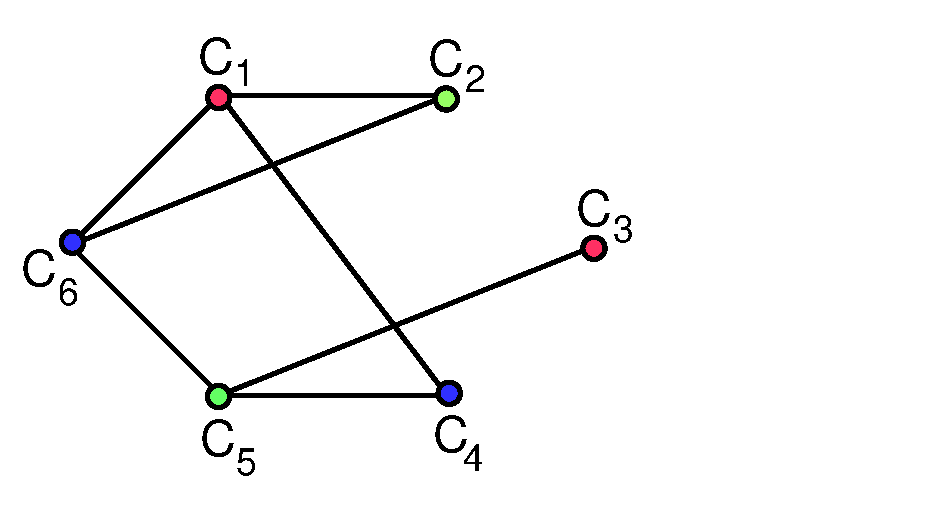
\includegraphics[scale=0.3]{color7.pdf}
%           \begin{tabular}{ccc}
%            Color 1 & Color 2 & Color 3 \\
%            $\bs{C_1}$ y $\bs{C_3}$ & $\bs{C_4}$ y $\bs{C_6}$ & $\bs{C_2}$ y $\bs{C_5}$
%           \end{tabular}
%%           \caption{\label{...}...}
%           \end{figure}
%
%
%\vspace{0.4cm}
%N�tese que no podemos obtener una coloración con menos colores pues el número cromático de este grafo tiene que ser $\bs{\geq 3}$ al contener a $\bs{K_3}$.
%\vspace{0.4cm}

\textbf{Complejidad del algoritmo voraz}
\vspace{0.3cm}

        \noindent En el paso $\bs{i}$ tenemos las operaciones:
        \begin{itemize}
        \item Adyacencias: $\bs{i-1}$
%        \vspace{-0.2cm}
        \item Pertenencias: $\bs{i-1}$
%        \vspace{-0.2cm}
        \item Sumas: $\bs{i-1}$
%        \vspace{-0.2cm}
        \item Asignaciones: $\bs{1+(i-1)+1+(i-1)+1}$
        \end{itemize}
\vspace{0.3cm}
        \noindent En total tenemos:
        \begin{itemize}
        \item Adyacencias:
        $\bs{1+2+\cdots+(n-2)+(n-1)=\frac{n(n-1)}{2} \mbox{  es  } O(n^2)}$
%        \vspace{-0.1cm}
        \item Pertenencias: $\bs{1+2+\cdots+(n-2)+(n-1)\mbox{  es  }O(n^2)}$
%        \vspace{-0.1cm}
        \item Sumas: $\bs{1+2+\cdots+(n-2)+(n-1) \mbox{  es  }O(n^2)}$
%        \vspace{-0.1cm}
        \item Asignaciones: $\bs{1+3(n-1)+2\left(1+2+\cdots+(n-2)+(n-1)\right)=}$\\
        $\bs{1+3n-3+n(n-1)=n^2+2n-2 \mbox{  es  }O(n^2)}$
        \end{itemize}

\vspace{0.4cm}
\subsubsection{\underline{árbol Spanning Minimal (A.S.M.)}}

Supongamos que queremos construir carreteras entre varias ciudades. Formalmente tenemos un grafo $\bs{G=(V,A)}$ cuyos vértices son las ciudades y las aristas las carreteras, y una función $\bs{w:A\rightarrow\mathbb{N}}$ de forma que $\bs{w(a)}$ representa el coste de la carretera $\bs{a}$. Decimos que $\bs{G}$ y $\bs{w}$ constituyen un grafo ponderado y que $\bs{w}$ es una función de peso.
\vspace{0.2cm}

El objetivo práctico es obtener una red de carreteras de coste mínimo, que se corresponde con el problema de obtener un árbol spanning $\bs{T=(V,A')}$ de $\bs{G}$ cuyo peso total $$\bs{w(T)=\sum_{a\in A'}w(a)}$$ sea el menor posible. Este problema tiene solución, sin embargo, pueden existir varios árboles spanning distintos cuyo peso total sea mínimo.
\vspace{0.6cm}

\noindent\textbf{Algoritmo voraz aplicado a un árbol Spanning Minimal:}
\vspace{0.3cm}

        \begin{enumerate}
            \item Primero tomamos la arista de menor peso.
            \item Después, en cada paso, se añade la arista de menor peso que añada un nuevo vértice al árbol parcial
            (si hay varias aristas posibles con el mismo peso, se elige cualquiera de ellas).
            \item Así con\-ti\-nua\-mos el proceso hasta completar los vértices del grafo de partida y teniendo cuidado de que no se formen ciclos
            para que el resultado final sea un árbol.
        \end{enumerate}

\vspace{0.2cm}

%      \begin{center}
%           \begin{figure}[h!]\centering
%           \noindent Apliquemos el algoritmo voraz al siguiente grafo:
%           \includegraphics[scale=0.2]{ASMb.pdf}
%%           \caption{\label{...}...}
%           \end{figure}
%      \end{center}
%
%
%      \begin{center}
%           \begin{figure}[h!]
%           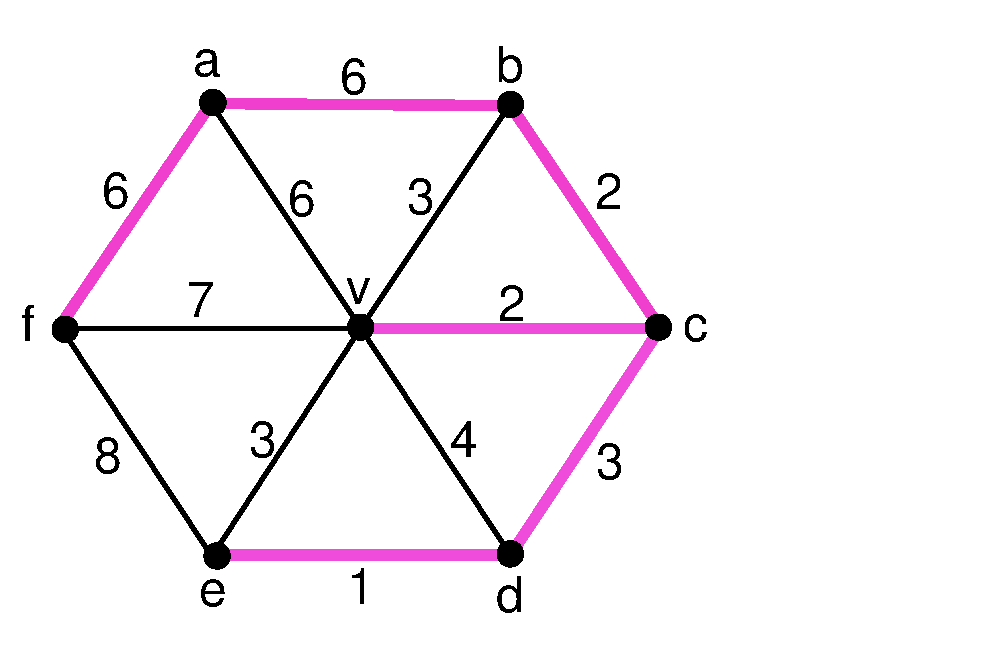
\includegraphics[scale=0.2]{ASM.pdf}
%           \noindent Partimos de la arista $\bs{de}$ (menor peso). Podemos añadir las aristas $\bs{dc}$ ó $\bs{ev}$ (peso 3)
%           y las aristas, en este orden, $\bs{dc}$, $\bs{cb}$, $\bs{cv}$, $\bs{ba}$, $\bs{af}$.
%%           \caption{\label{...}...}
%           \end{figure}
%      \end{center}

%\vspace{-2cm}
\begin{teorema}
Sea $\bs{G=(V,A)}$ un grafo ponderado conexo con función de peso $\bs{w:A\rightarrow\mathbb{N}}$. Supongamos que $\bs{T}$ es un árbol
spanning de $\bs{G}$ que resulta de aplicarle el algoritmo voraz. Entonces se verifica:

        $$\bs{w(T)\leq w(U)}$$

para cualquier otro árbol $\bs{U}$ spanning de $\bs{G}$.
\end{teorema}

\subsection{Algoritmos de búsqueda}

Supongamos que hemos de llevar a cabo la búsqueda de los vértices de un grafo em\-pe\-zan\-do en un vértice concreto.
Podemos emplear dos estrategias distintas:
        \begin{itemize}
            \item podríamos ``profundizar'', moviéndonos a un nuevo vértice siempre que fuera posible, o
            \vspace{-0.2cm}
            \item podríamos ``desplegarnos'' comprobando todos los vértices en un ``nivel'' antes de pasar al siguiente.
        \end{itemize}

\vspace{0.2cm}
La primera estrategia se conoce con el nombre de \textbf{búsqueda en profundidad} (B.E.P.) y la segunda con el nombre de
\textbf{búsqueda en anchura} (B.E.A.).
\vspace{0.2cm}

La siguiente figura representa una habitación con siete juguetes escondidos, el problema consiste en encontrar los juguetes representados por las
letras $\bs{a}$, $\bs{b}$, $\bs{c}$, $\bs{d}$, $\bs{e}$, $\bs{f}$ y $\bs{g}$.

%\vspace*{0.5cm}

      \begin{center}
           \begin{figure}[h!]\centering
           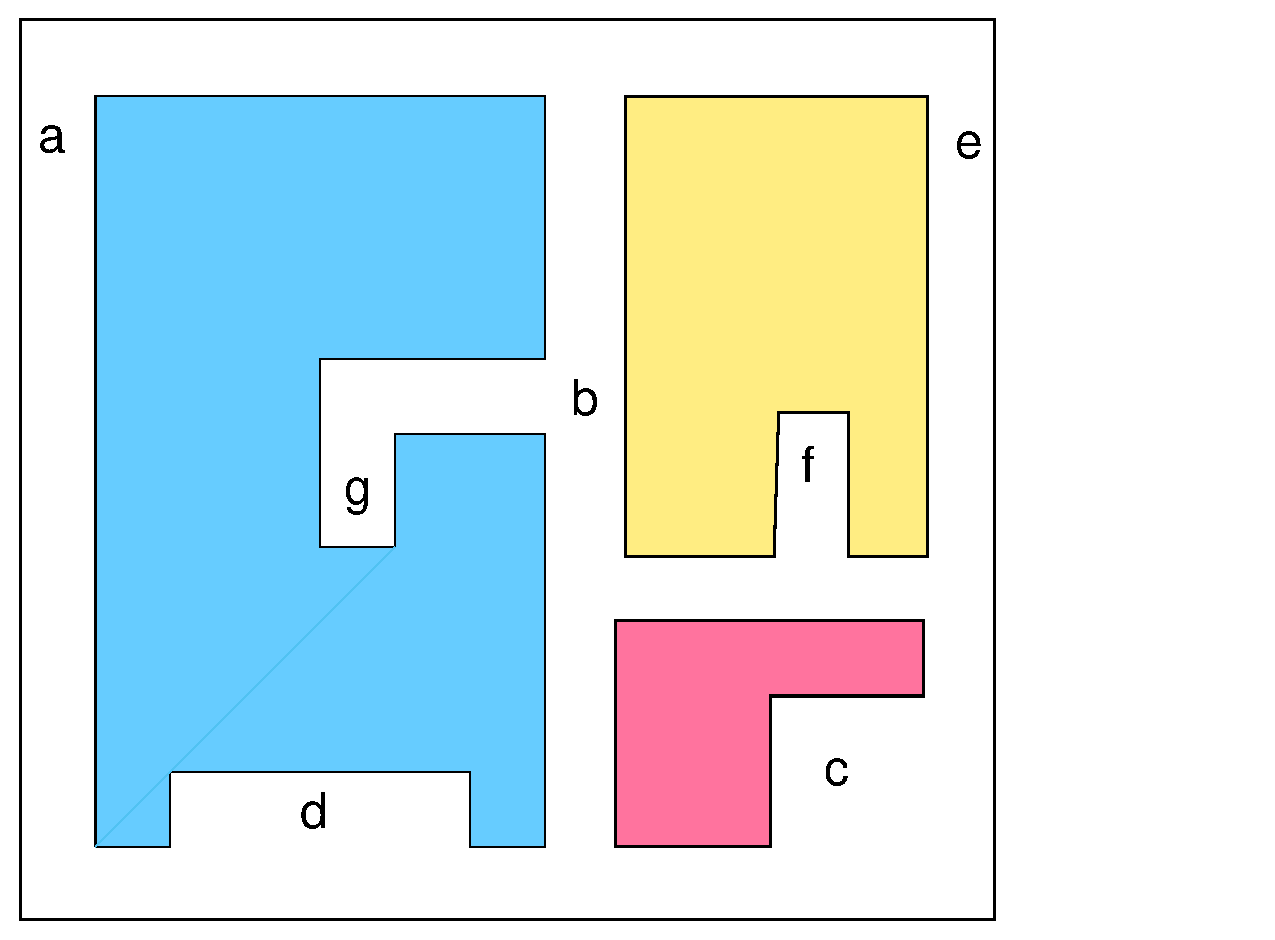
\includegraphics[scale=0.14]{pdfs/B1.pdf}
%           \caption{\label{...}...}
           \end{figure}
      \end{center}


\vspace{0.5cm}
Podemos representar esta situación mediante un grafo, donde los vértices serán los juguetes y las aristas representan las rutas disponibles entre los juguetes.
\vspace{0.2cm}

Para el ejemplo dado tendríamos el siguiente grafo:

      \begin{center}
           \begin{figure}[h!]\centering
           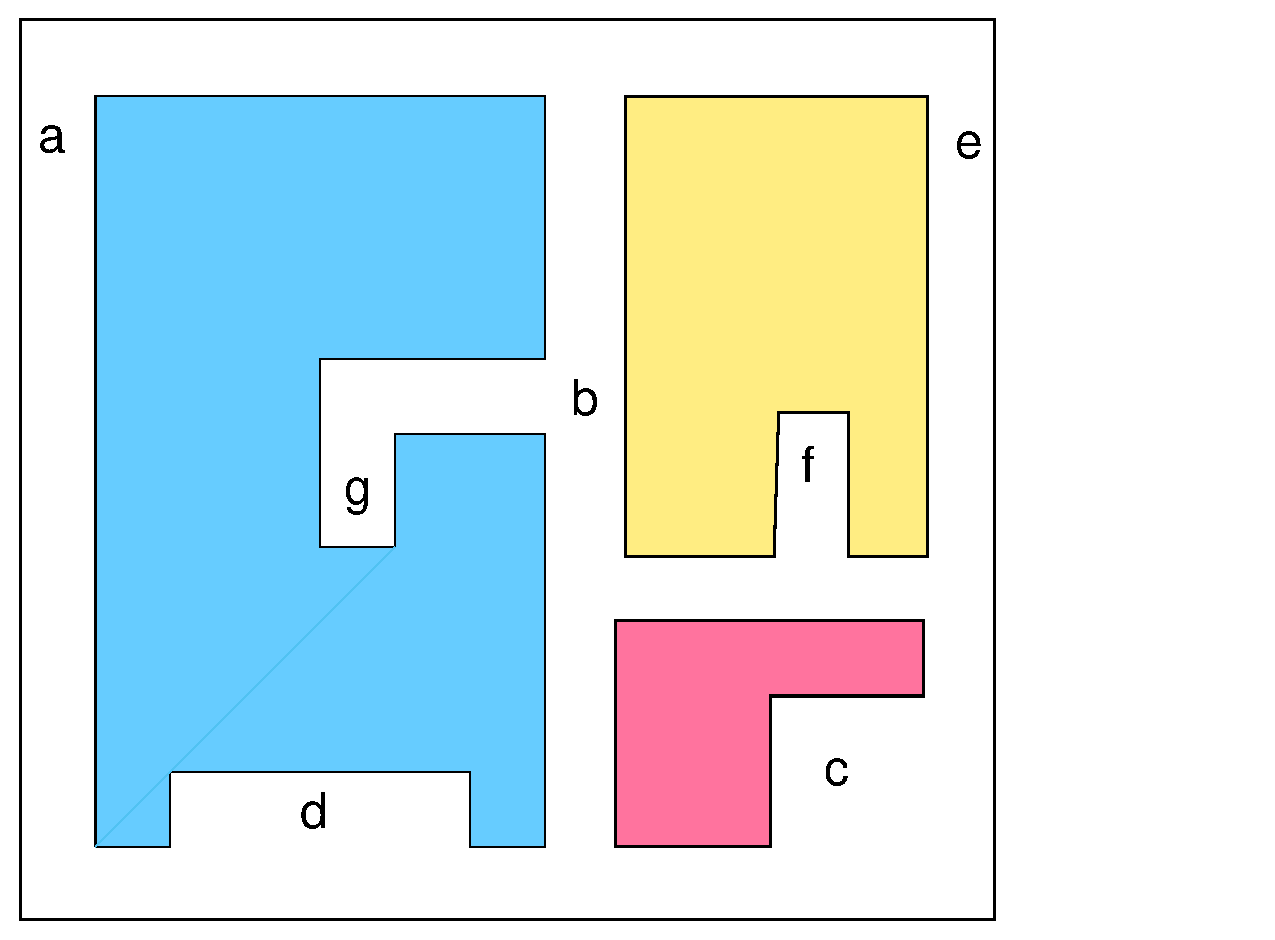
\includegraphics[scale=0.15]{pdfs/B1.pdf}
           \includegraphics[scale=0.2]{pdfs/B2.pdf}
%           \caption{\label{...}...}
           \end{figure}
      \end{center}


%\vspace{0.2cm}
\newpage
\noindent\underline{\textbf{Algoritmo Búsqueda en Profundidad (B.E.P.)}}:

        \begin{quotation}
        \noindent $\bs{Q:=v}$\\[1ex]
        \textsf{Mientras} $\bs{Q\neq\emptyset}$ \textsf{haz}\\[1ex]
        \hspace*{5ex} $\bs{x:=\mbox{ Ultimo}(Q)}$\\[1ex]
        \hspace*{5ex} \textsf{Si} $\bs{x}$ es adyacente a un nuevo vértice $\bs{y}$\\[1ex]
        \hspace*{10ex} \textsf{entonces} $\bs{Q:=(Q\mbox{ seguida de }y)}$\\[1ex]
        \hspace*{10ex} \textsf{y en otro caso} $\bs{Q:=(Q\mbox{ con }x\mbox{ eliminado})}$
        \end{quotation}

\vspace{0.4cm}
        B.E.P. $\rightarrow$ D.F.S. = Depth First Search
%\vspace{0.4cm}
%
%        \begin{center}
%        \begin{figure}[h!]\centering
%        \includegraphics[scale=0.2]{B2.pdf}
%        \begin{minipage}{.4\textwidth}\begin{tabular}{|ccl|} \hline
%            A\~nadir & Quitar & $\bs{Q}$ \\ \hline
%            $\bs{a}$ & -- & $\bs{a}$ \\
%            $\bs{b}$ & -- & $\bs{ab}$ \\
%            $\bs{c}$ & -- & $\bs{abc}$ \\
%            $\bs{e}$ & -- & $\bs{abce}$ \\
%            $\bs{f}$ & -- & $\bs{abcef}$ \\
%            -- & $\bs{f}$ & $\bs{abce}$ \\
%            -- & $\bs{e}$ & $\bs{abc}$ \\
%            -- & $\bs{c}$ & $\bs{ab}$ \\
%            $\bs{d}$ & -- & $\bs{abd}$ \\
%            -- & $\bs{d}$ & $\bs{ab}$ \\
%            $\bs{g}$ & -- & $\bs{abg}$ \\
%            -- & $\bs{g}$ & $\bs{ab}$ \\
%            -- & $\bs{b}$ & $\bs{a}$ \\
%            -- & $\bs{a}$ & $\bs{\emptyset}$ \\ \hline
%        \end{tabular}\end{minipage}
%        \end{figure}
%        \end{center}

\vspace{1cm}
\noindent\underline{\textbf{Algoritmo Búsqueda en Anchura (B.E.A.)}}:

        \begin{quotation}
        \noindent $\bs{Q:=v}$\\[1ex]
        \textsf{Mientras} $\bs{Q\neq\emptyset}$ \textsf{haz}\\[1ex]
        \hspace*{5ex} $\bs{x:=\mbox{ Primero}(Q)}$\\[1ex]
        \hspace*{5ex} \textsf{Si} $\bs{x}$ es adyacente a un nuevo vértice $\bs{y}$\\[1ex]
        \hspace*{10ex} \textsf{entonces} $\bs{Q:=(Q\mbox{ seguida de }y)}$\\[1ex]
        \hspace*{10ex} \textsf{y en otro caso} $\bs{Q:=(Q\mbox{ con }x\mbox{ eliminado})}$
        \end{quotation}

\vspace{0.4cm}
        B.E.A. $\rightarrow$ B.F.S. = Breadth First Search
\vspace{0.4cm}
%
%        \begin{center}
%        \begin{figure}[h!]\centering
%        \includegraphics[scale=0.2]{B2.pdf}
%        \begin{minipage}{.4\textwidth}\begin{tabular}{|ccl|} \hline
%            A\~nadir & Quitar & $\bs{Q}$ \\ \hline
%            $\bs{a}$ & -- & $\bs{a}$ \\
%            $\bs{b}$ & -- & $\bs{ab}$ \\
%            $\bs{d}$ & -- & $\bs{abd}$ \\
%            -- & $\bs{a}$ & $\bs{bd}$ \\
%            $\bs{c}$ & -- & $\bs{bdc}$ \\
%            $\bs{e}$ & -- & $\bs{bdce}$ \\
%            $\bs{f}$ & -- & $\bs{bdcef}$ \\
%            $\bs{g}$ & -- & $\bs{bdcefg}$ \\
%            -- & $\bs{b}$ & $\bs{dcefg}$ \\
%            -- & $\bs{d}$ & $\bs{cefg}$ \\
%            -- & $\bs{c}$ & $\bs{efg}$ \\
%            -- & $\bs{e}$ & $\bs{fg}$ \\
%            -- & $\bs{f}$ & $\bs{g}$ \\
%            -- & $\bs{g}$ & $\bs{\emptyset}$ \\ \hline
%        \end{tabular}\end{minipage}
%        \end{figure}
%        \end{center}
%
%
%\vspace{0.2cm}
        En la B.E.P. la lista de vértices se conoce con el nombre de pila, ya que se comporta como una pila de platos,
        sólo se pueden añadir o quitar vértices (platos) en la cima de la pila.
\vspace{0.2cm}

        La B.E.A. se comporta como una cola, ya que recuerda a una cola de personas esperando en una tienda a ser atendidos. Los nuevos
        vértices se añaden al final de la cola y los antiguos se eliminan del principio.
\vspace{0.2cm}

        \begin{itemize}
            \item B.E.P. $\rightarrow$ LIFO=Last in, first out (la última que llega es la primera que sale)
            \item B.E.A. $\rightarrow$ FIFO=First in, first out (la primera que llega es la primera que sale)
        \end{itemize}

\vspace{0.2cm}
Los procedimientos de búsqueda pueden u\-ti\-li\-zar\-se para ver si un grafo $\bs{G}$ es conexo o no. Ya que si al final hemos pasado por todos
los vértices de $\bs{G}$, es decir, hemos obtenido un árbol spanning, entonces $\bs{G}$ es conexo.

%\vspace{0.2cm}
%Los árboles spanning (en trazo de color) que se obtienen para el grafo del ejemplo son:
%
%      \begin{center}
%           \begin{figure}[h!]\centering
%           \includegraphics[scale=0.2]{BEP.pdf}
%           \includegraphics[scale=0.2]{BEA.pdf}
%%           \caption{\label{...}...}
%           \end{figure}
%      \end{center}
%
%\vspace{0.2cm}
%Los árboles anteriores, si los consideramos enraizados con raíz en $\bs{a}$, quedarían:
%
%      \begin{center}
%           \begin{figure}[h!]\centering
%           \includegraphics[scale=0.22]{BEP2.pdf}
%           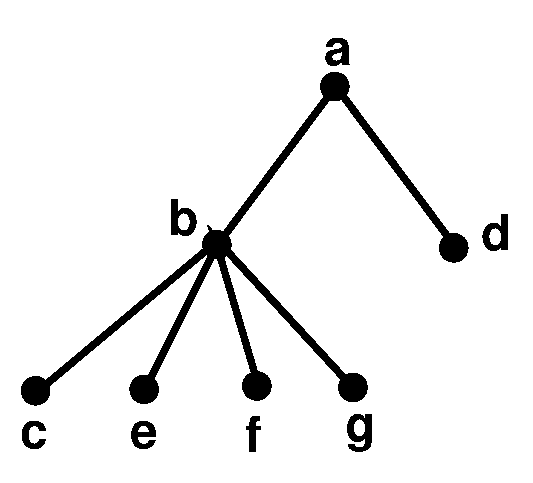
\includegraphics[scale=0.22]{BEA2.pdf}
%%           \caption{\label{...}...}
%           \end{figure}
%      \end{center}

\newpage

\section{Cierre Convexo de una nube de puntos. Algoritmos.}

\subsection{Cierre Convexo (Convex Hull).}

\begin{defi} Un conjunto $A \subseteq \mathbb{R}^d$ se dice
\textbf{convexo} si $\overline{xy} \subseteq A$, $\forall x,y \in A$.
\end{defi}

\begin{prop} La intersección de una familia de
conjuntos convexos es un conjunto convexo.
\end{prop}

\begin{defi} El \textbf{cierre convexo} de un conjunto $S$
es el menor convexo que contiene a $S$. Lo notaremos: $\textbf{CH(S)}$.
\end{defi}

\begin{prop} $CH(S)$ es la intersección de todos los
conjuntos convexos que contienen a $S$.
\end{prop}

\begin{nota} A continuación, veamos el cierre convexo para:
$$S \ = \ \mbox{nube de $n$ puntos en } \mathbb{R}^2$$
\end{nota}

\begin{prop} Si $P$ es un polígono convexo cuyos
vértices son puntos de $S$, entonces $P\subseteq CH(S)$.
\end{prop}

\begin{prop} Sea $P$ un polígono convexo que contiene
a $S$ y cuyos vértices son puntos de $S$. Entonces $P=CH(S)$. En
particular, $P$ es único.
\end{prop}

\begin{prop} La \textbf{envolvente convexa} de $S$ es la
frontera de $CH(S)$.
\end{prop}

\begin{defi} Dados un conjunto $A \subseteq \mathbb{R}^2$ y un
punto $p \in A$, se dice que una recta que pasa por $p$ es
\textbf{soporte} de $A$ si todos los puntos de $A$ quedan en uno de los
semiplanos cerrados determinados por dicha recta.
\end{defi}

\begin{teorema} Sea $P$ un polígono cuyos vértices están
ordenados con orientación positiva. Son equivalentes:
\begin{enumerate}
  \item $P$ es convexo.
  \item Toda recta que pase por dos vértices consecutivos deja a $P$
en el semiplano de la izquierda.
  \item Toda recta que pase por dos vértices consecutivos deja al
siguiente vértice de $P$ en el semiplano de la izquierda.
  \item Todo ángulo interior en cada vértice de $P$ es menor o igual
que $\pi$.
  \item Todo vértice admite una recta soporte de $P$ que pasa por
él.
\end{enumerate}
\end{teorema}


\subsubsection{área signada de un triángulo}

\noindent Dados tres puntos $$p_1=(x_1,y_1), \quad p_2=(x_2,y_2), \quad p_3=(x_3,y_3)$$ en el plano, el área del triángulo que determinan viene dada por
$$\mbox{área} \ = \ \frac{1}{2} {\rm abs}\left(\Delta(p_1,p_2,p_3)\right),$$
siendo $$\Delta(p_1,p_2,p_3) \ = \ \left| \begin{array}{ccc}
1 & 1 & 1 \\
x_1 & x_2 & x_3 \\
y_1 & y_2 & y_3
\end{array}
\right|$$
el \textbf{área signada}. Su signo coincide con el del vector $\overrightarrow{p_1p_2}\wedge\overrightarrow{p_1p_3}$ y sirve para orientar el triángulo
de vértices $p_1p_2p_3$:
\begin{itemize}
   \item Si $\Delta(p_1,p_2,p_3)>0$, entonces $(p_1,p_2,p_3)$ tiene orientación positiva.
   \item Si $\Delta(p_1,p_2,p_3)<0$, entonces $(p_1,p_2,p_3)$ tiene orientación negativa.
\end{itemize}

\subsection{Algoritmos.}

\subsubsection{\underline{Algoritmo de {\it \textbf{fuerza bruta}}}}

{\bf Descripción:}

\begin{itemize}
  \item \textbf{Paso 1:} Para cada par de puntos de $S$ se comprueba si todos los
demás están en un mismo semiplano de los dos que determina la
recta que pasa por ellos. Si es así, determinan un lado de la
envolvente y si no, no.
  \item \textbf{Paso 2:} Se ordenan los lados para que aparezcan tal y
como lo hacen al recorrer la frontera.
\end{itemize}


{\bf Complejidad:}

\begin{itemize}
  \item \textbf{Paso 1:} $O(n)$ para cada par de puntos. Como hay
$\left(\begin{array}{c}n\\2\end{array}\right)$ pares, $O(n^3)$
para encontrar el conjunto de vértices de la envolvente convexa.
  \item \textbf{Paso 2:} $O(n\log n)$ en el peor de los casos.
  \item \textbf{Total:} $O(n^3)$.
\end{itemize}


\subsubsection{\underline{Marcha de Jarvis}}

{\bf Idea:} Partiendo de un vértice de la envolvente, se
busca otro vértice que con él determine una recta soporte de $S$.

\vspace{0.5cm}

{\bf Descripción:}
\begin{itemize}
  \item \textbf{Entrada:} $S=(p_1,\dots,p_n)$.
  \item \textbf{Salida:} Lista cíclica con los vértices de la envolvente
convexa de $S$: $C=(v_1,\dots,v_k)$.
  \item \textbf{Paso 0:} Encontrar el punto de $S$ con abscisa mínima (si
hubiera más de uno, el de menor ordenada): será $v_1$ que
insertaremos en $C$, inicialmente vacía.
  \item \textbf{Paso i:} Localizar en $S$ el punto de menor ángulo positivo
respecto a $v_i$ y al rayo $r_i$ que emana de $v_i$ con la
dirección $\overrightarrow{v_{i-1}v_i}$, si $i\neq 1$, y si $i=1$,
al rayo vertical $r_1$ que emana de $v_1$ en la dirección de
$-\infty$ (si hubiera más de uno, el que esté más alejado de
$v_i$). Ese punto será $v_{i+1}$. Si $v_{i+1}\neq v_1$, lo
insertamos en $C$ y continuamos. En caso contrario, hemos acabado.
\end{itemize}

{\bf Corrección:}

\begin{itemize}
%\item Para cada $i$, $v_i$ es un vértice de la envolvente convexa
%y $r_i$ es recta soporte de $S$.
  \item $C$ es la frontera de un polígono convexo con vértices en
$S$ y que contiene a $S$.
\end{itemize}


{\bf Complejidad:}

\begin{itemize}
  \item \textbf{Paso 0:} Puede hacerse en tiempo $O(n)$.
  \item \textbf{Paso i:} Para cada $i$, puede hacerse en tiempo $O(n)$.
  \item \textbf{Total}: $O(n\cdot k)$, donde $k$ es el número de vértices en la
envolvente convexa. $O(n^2)$ en el peor de los casos.
\end{itemize}



\begin{observaciones}
\begin{itemize}
\item El cálculo para encontrar el mínimo angular puede hacerse
usando áreas signadas.
\end{itemize}
$$\angle (\overrightarrow{v_ip_j},r_i) <
\angle (\overrightarrow{v_ip_k},r_i) \Leftrightarrow
\Delta(v_i,p_j,p_k)>0$$
\end{observaciones}

\subsubsection{\underline{Scan de Graham}}

\begin{itemize}
  \item Un polígono convexo es estrellado. Por tanto, los vértices
aparecen ordenados angularmente respecto a cualquier punto del
núcleo.
  \item Un polígono convexo es monótono respecto a cual\-quier
dirección. Por tanto, su frontera puede des\-com\-po\-ner\-se en
dos cadenas monótonas respecto de OX. En cada una, los vértices
están ordenados por abscisas.
  \item Todos los vértices de un polígono convexo son convexos.
\end{itemize}

\vspace{0.6cm}

{\bf Idea:}

\begin{enumerate}
  \item \textbf{Ordenación:} Obtener una lista cíclica $L$ con todos los puntos de
$S$ de manera que describa un polígono estrellado o monótono.
  \item \textbf{Scan:} Quitar de $L$ los puntos que no formen con sus dos
adyacentes un ángulo menor que $\pi$.
\end{enumerate}


{\bf Descripción:}

Suponemos que en $S$ no hay más de dos puntos alineados.

\begin{itemize}
  \item\textbf{Entrada:} $S=(p_1,\dots,p_n)$.
  \item\textbf{Salida:} Lista cíclica con los vértices de la envolvente
convexa de $S$: $C=(v_1,\dots,v_k)$.
  \item\textbf{Paso 1:} Encontrar el punto de $S$ con abscisa mínima (si
hubiera más de uno, el de menor ordenada): será $v_1$ que
insertaremos en $C$, inicialmente vacía.
  \item\textbf{Paso 2:} Ordenar angularmente el resto de puntos de $S$
res\-pec\-to a $v_1$ y en sentido positivo respecto al rayo
vertical que emana de él en dirección a $-\infty$. Sea
$L=(v_1,\dots,v_n)$ el resultado.
  \item\textbf{Paso 3:} Insertar $v_2$ en $C$. Hacer $q=v_2$.
  \item\textbf{Paso 4:} (Scan) Desde $i=3$ hasta $n$, hacer
\begin{enumerate}
  \item $p=ant(q)$ (anterior en $C$).
  \item Mientras $\Delta(p,q,v_i) \leq 0$,
\begin{enumerate}
  \item Borrar $q$ de $C$.
  \item Actualizar $q=p$ y $p=ant(q)$.
\end{enumerate}
  \item Insertar $v_i$ en $C$ y actualizar $q=v_i$.
\end{enumerate}
\end{itemize}

\begin{itemize}
  \item Obsérvese que con la ordenación del Paso 2, tanto $v_2$ como
$v_n$ son vértices de la envolvente.
\end{itemize}
\vspace{0.2cm}

{\bf Nota:}

Si en $S$ hay más de dos puntos alineados, basta
modificar el algoritmo de modo que en el paso de ordenación
angular, cuando haya varios puntos con el mismo ángulo, nos
quedemos sólo con el más alejado de $v_1$.
\vspace{1cm}

{\bf Corrección:}

\begin{itemize}
  \item Los puntos que elimina el algoritmo no son vértices de la
envolvente convexa.
  \item Al finalizar el algoritmo, $C$ es un polígono convexo, pues
todos sus vértices son convexos. Además, sus vértices son puntos
de $S$. Para probar que $C=CH(S)$, basta ver que $S \subseteq C$.
\end{itemize}

{\bf Complejidad:}

\begin{itemize}
  \item\textbf{Paso 1:} Puede hacerse en tiempo $O(n)$.
  \item\textbf{Paso 2:} Puede hacerse en tiempo $O(n\log n)$.
  \item\textbf{Scan:} El coste es $O(n)$ (el número máximo de test de
áreas signadas es $2n-4$).
  \item\textbf{Total:} $O(n\log n)$.
\end{itemize}

\subsubsection{Algoritmos: Scan de Graham - Variante}

\begin{itemize}
  \item\textbf{Entrada:} $S=(p_1,\dots,p_n)$.
  \item\textbf{Salida:} Lista cíclica con los vértices de la envolvente
convexa de $S$: $C=(v_1,\dots,v_k)$.
  \item\textbf{Paso 1:} Ordenar lexicográficamente los puntos de $S$
obteniendo la lista $L$.
  \item\textbf{Paso 2:} Aplicar el scan a $L$ y obtener $C_1$, que es
cadena inferior de la envolvente convexa.
  \item\textbf{Paso 3:} Invertir el orden en $L$ obteniendo $L'$. Aplicar
el scan a $L'$ y obtener $C_2$, que es cadena superior de la
envolvente convexa.
  \item\textbf{Paso 4:} Concatenar $C_1$ y $C_2$ eliminando las
repeticiones de los extremos para obtener la lista $C$.
\end{itemize}

\subsubsection{Algoritmos: Scan de Graham - Variante de Akl-Toussaint}

\begin{itemize}
  \item Antes de ordenar, localizar los puntos extremales (abscisas
y ordenadas mínimas y máximas). Estos puntos determinan un convexo
contenido en $CH(S)$.
  \item Eliminar los puntos de $S$ que están en el interior de dicho
convexo.
  \item Con los que quedan, se continúa como en el algoritmo
anterior, actuando sobre listas parciales.
  \item El coste del paso adicional es $O(n)$, por lo que la
complejidad sigue siendo $O(n\log n)$.
\end{itemize}


\section{Cálculo del diámetro de una nube de puntos.}

\subsection{Diámetro de una nube de puntos}

\begin{defi} El \textbf{diámetro} de una nube de $n$
puntos es la mayor distancia entre dos de ellos. Es decir, si
$S=\{p_1,\dots,p_n\}$, $$diam(S) \ = \ \displaystyle{{\rm max}_{1\leq i,j \leq
n}}d(p_i,p_j)$$
\end{defi}

{\bf Algoritmo de ``fuerza bruta":}

\begin{enumerate}
  \item Para cada par de puntos $p_i,p_j$, hallar $d(p_i,p_j)$.
  \item Tomar el mayor de los valores obtenidos.
\end{enumerate}

{\bf Complejidad:} $O(n^2)$.

\begin{prop} El diámetro de $S$ se alcanza en vértices
de $CH(S)$.
\end{prop}

\subsection{Diámetro de un polígono convexo}

Sea $P$ un polígono convexo de $n$ vértices.

 $$diam(P)\ = \ {\rm max}\{d(p,q)\ / \ p,q \in P\}$$

\

\begin{prop} $diam(P) \ = \  diam(\{\mbox{vértices de
}P\})$.
\end{prop}

\begin{defi} Se dice que dos vértices $p,q$ de $P$ son
\textbf{antípodas} si existen dos rectas paralelas distintas que
pasan por esos puntos y son soporte de $P$.
\end{defi}

\begin{prop} Si $diam(P)=d(p,q)$, entonces $p$ y $q$
son antípodas.
\end{prop}

{\bf Algoritmo:}

\begin{enumerate}
  \item Hallar todos los pares de antípodas de $P$.
  \item Hallar la distancia entre los puntos de cada par.
  \item Tomar el mayor de los valores obtenidos.
\end{enumerate}


\subsection{Algoritmo de girar calibres}


\begin{nota} La comparación entre los ángulos $\alpha$ y $\beta$ se puede hacer
usando áreas signadas

 $$\alpha<\beta \Leftrightarrow \Delta(p,SIG(p),x)<0$$

 $$x=p+\overrightarrow{qSIG(q)}$$

\end{nota}

\begin{itemize}
  \item\textbf{Entrada:} Lista cíclica $P$ con los $n$ vértices de un polígono
convexo en orientación positiva.
  \item\textbf{Salida:} Lista $Q$ con las parejas de antípodas de $P$.
  \item\textbf{Paso 1:} Hacer $Q:=\emptyset$.
  \item\textbf{Paso 2:} Localizar en $P$ los puntos mínimo y máximo con orden
lexicográfico: $x_{min}$ y $x_{max}$.
  \item\textbf{Paso 3:} Hacer $p:=x_{min}$ y $q:=x_{max}$.
  \item\textbf{Paso 4:} Mientras $q\neq x_{min}$ o $p\neq x_{max}$ repetir:
\begin{itemize}
  \item Introducir en $Q$ el par $(p,q)$.
  \item Hacer $x:=p+\overrightarrow{qSIG(q)}=p+SIG(q)-q$.
  \item Si $\Delta(p,SIG(p),x)<0$, hacer $p:=SIG(p)$
  \item Si $\Delta(p,SIG(p),x)>0$, hacer $q:=SIG(q)$
  \item Si $\Delta(p,SIG(p),x)=0$, añadir a $Q$ los pares $(p,SIG(q))$ y
$(SIG(p),q)$ y hacer $p:=SIG(p)$ y $q:=SIG(q)$.
\end{itemize}
  \item\textbf{Paso 5:} Acabar devolviendo $Q$.
\end{itemize}

{\bf Corrección:} El algoritmo acaba.

{\bf Complejidad:} $O(n)$.

\section{Problemas de proximidad}

Dada una nube $S$ con $n$ puntos, se plantean los si\-guien\-tes
problemas:


\begin{enumerate}

  \item Fijado un punto de $S$, encontrar la región del plano
formada por los puntos que están más próximos a él que a cualquier
otro de $S$.

  \item \textbf{Todos los vecinos más cercanos:} Para cada punto de $S$ encontrar cuál es su punto más cercano.

  \item \textbf{El par más cercano:} Encontrar el par de puntos de $S$ cuya distancia entre sí sea mínima.

  \item \textbf{El vecino más cercano:} Dado un nuevo punto $p$,
encontrar el elemento de $S$ más cercano a $p$.

  \item \textbf{Mayor círculo vacío:} Encontrar el mayor círculo que no contenga ningún punto de $S$ y cuyo centro esté dentro de $CH(S)$.

  \item \textbf{Triangulación:} Encontrar una triangulación que contenga a los puntos de $S$ como vértices.

  \item \textbf{árbol spanning mínimo:} Construir un árbol de longitud mínima que tenga a los puntos de $S$ como vértices.

\end{enumerate}

\subsection{Diagrama de Voronoi}

$$S = \{ p_1, \dots ,p_n \} \subset \mathbb{R}^2$$

\begin{defi}Se llama \textbf{región}, \textbf{célula} o \textbf{polígono de Voronoi} de  $p_i$ al conjunto

\vspace{-0.2cm}

$$Vor(p_i)=\{q\in \mathbb{R}^2 | d(q,p_i) \leq d(q,p_j), \forall j \neq i \}$$.

\end{defi}

\vspace{-0.1cm}

Denotamos por $h(p_i,p_j)$ al semiplano que contiene a $p_i$ y
tiene por borde la mediatriz $m_{ij}$ del segmento
$\overline{p_ip_j}$.

\begin{lemma} Se verifica:

$$Vor(p_i)= \bigcap _{j\neg i} h(p_i,p_j)$$


\end{lemma}

\begin{defi} Se llama \textbf{diagrama de Voronoi} de $S$,
$Vor(S)$, a la teselación del plano determinada por la familia
$\{Vor(p_i)\}_{i=1,\dots,n}$. Los puntos $p_i$ se llaman \textbf{generadores} del diagrama, y los vértices y segmentos o
semirrectas de $Vor(S)$ se llaman \textbf{vértices} y \textbf{aristas de Voronoi} de $S$, respectivamente.
\end{defi}

\begin{nota}
\begin{itemize}

  \item El diagrama de Voronoi constituye una partición del plano en polígonos convexos (los polígonos de Voronoi), tal que cada punto de $S$ pertenece a un único polígono.

  \item Cada arista de $Vor(S)$ es común a dos polígonos y es perpendicular al segmento que une los puntos de $S$ que están en estos polígonos.

  \item $Vor(S)$ contiene toda la información de proximidad relativa a $S$.

  \item El diagrama de Voronoi se puede definir en dimensiones superiores.

\end{itemize}
\end{nota}

\vspace{0.3cm}
\noindent Además, suponiendo que los puntos de $S$ están en posición general:

\begin{itemize}

  \item Los puntos de $S$ no están todos alineados.

  \item No hay cuatro puntos de $S$ que sean cocirculares.

\end{itemize}

\begin{teorema} Cada vértice del diagrama de Voronoi es la intersección de tres aristas del diagrama.
\end{teorema}

\begin{nota} Los vértices de Voronoi son los centros de
circunferencias definidas por tres puntos de $S$.
\end{nota}


\begin{teorema} Para cada vértice $v$ de $Vor(S)$, la
circunferencia correspondiente no contiene a ningún otro punto de
$S$.
\end{teorema}

\begin{teorema} Para cada $p_i \in S$, cada vecino más
próximo a $p_i$ define una arista en el polígono $Vor(p_i)$.
\end{teorema}

\begin{teorema} El polígono $Vor(p_i)$ es no acotado si y
sólo si $p_i$ es un punto de la envolvente convexa de $S$.
\end{teorema}

\begin{coro} Las semirrectas de $Vor(S)$ corresponden a
pares de puntos adyacentes de la envolvente convexa de $S$.
\end{coro}

\subsection{Triangulación de Delaunay}

\begin{defi} El grafo dual de $Vor(S)$ recibe el nombre de \textbf{grafo de Delaunay} de $S$.
\end{defi}

\begin{teorema} Si los puntos de $S$ están en posición
ge\-ne\-ral, el grafo dual de $Vor(S)$ es una triangulación de
$S$, llamada \textbf{triangulación de Delaunay} de $S$.
\end{teorema}

\textbf{\underline{Solución de los problemas de proximidad}}

\begin{itemize}

  \item Fijado un punto de $S$, encontrar la región del plano formada por los puntos que están más próximos a él que a cualquier otro de $S$.

  \item[\textbf{Sol.:}] Dado $p_i \in S$, dicha región es $Vor(p_i)$.


  \item \textbf{Todos los vecinos más cercanos:} Para cada punto de $S$ encontrar cuál es su punto más cercano.

  \item[\textbf{Sol.:}] Los vecinos más próximos a $p_i$ definen las aristas de $Vor(p_i)$, por lo que bastará conocer dichas aristas.


  \item \textbf{El par más cercano:} Encontrar el par de puntos de $S$ cuya distancia entre sí sea mínima.

  \item[\textbf{Sol.:}] Se resuelve en tiempo lineal una vez conocida la solución del
problema anterior.


  \item \textbf{El vecino más cercano:} Dado un nuevo punto $p$,
encontrar el elemento de $S$ más cercano a $p$.

  \item[\textbf{Sol.:}] Basta determinar en qué región de $Vor(S)$ se encuentra $p$.


  \item \textbf{Mayor círculo vacío:} Encontrar el mayor círculo que no contenga ningún punto de $S$ y cuyo centro esté dentro de $CH(S)$.

  \item[\textbf{Sol.:}] Se define la función $f(x,y)$ como la distancia del punto $(x,y)$ a su punto más cercano de $S$ y se prueba que $f$ (restringida a $CH(S)$) alcanza su máximo en un vértice de uno de los polígonos que se obtienen al hallar $Vor(S)\cap CH(S)$.


  \item \textbf{Triangulación:} Encontrar una triangulación que contenga a los puntos de $S$ como vértices.

  \item[\textbf{Sol.:}] Considerar la Triangulación de Delaunay.


  \item \textbf{árbol spanning mínimo:} Construir un árbol de longitud mínima que tenga a los puntos de $S$ como vértices.

  \item[\textbf{Sol.:}] Puede obtenerse a partir de la Triangulación de Delaunay, con el siguiente procedimiento: elegido un árbol $T$, localizar la arista $(u',v')$ tal que $d(u',v')={\rm min}\{d(u,v) \ / \ u\in T, \ v\in S\setminus T\}$.

\end{itemize}


\subsection{Algoritmos}

\textbf{1. \underline{Divide y vencerás}:}

\begin{itemize}

  \item \textbf{Paso 1:} Dividir el conjunto $S$ en dos subconjuntos $S_1$ y $S_2$ (con igual número de puntos, aproximadamente) se\-pa\-ra\-dos por una recta vertical, de manera que $S_1$ quede a la izquierda de dicha recta.

  \item \textbf{Paso 2:} Construir $Vor(S_1)$ y $Vor(S_2)$.

  \item \textbf{Paso 3:} Construir la cadena poligonal $\sigma$ que separa $S_1$ y $S_2$.

  \item \textbf{Paso 4:} Obtener $Vor(S)$ como $$(Vor(S_1)\cap\pi_L)\cup (Vor(S_2)\cap\pi_R)$$ donde $\pi_L$ (resp. $\pi_R$) es la región del plano que queda a la izquierda (resp. derecha) de $\sigma$.

\end{itemize}

 Para detalles sobre el Paso 3, la corrección y la
complejidad de este algoritmo, véase: {\sc F. P. Preparata, M. I.
Shamos}. {\it Computational Geometry. An Introduction.}
Springer-Verlag, New York, 1985. Páginas 205-214.

\vspace{0.3cm}

\textbf{2. \underline{Fortune}:}

\vspace{0.3cm}

Véase: {\sc M. Berg et al.} {\it Computational
Geometry: Algorithms and Applications.} Springer-Verlag, Berlin,
2000.

\chapter{Modelado Geométrico}


\section{Introducción al Modelado}

\subsection{Curvas Paramétricas}

\begin{defi}
Una curva parametrizada regular de clase $C^k$  es una aplicación
\begin{center}
\begin{tabular}{cccl}
$\alpha:$ & $I$ & $\longrightarrow$ &$\mathbb{R}^3$ \\
 & $t$ & $\mapsto$ & $\alpha (t)
=(x(t),y(t),z(t))$
\end{tabular}
\end{center}

donde $I\subseteq {\mathbb{R}}$ es un intervalo abierto ($I=\mathbb{R} $ es posible), que verifica las siguientes condiciones:

\begin{enumerate}
\item $\alpha$ es diferenciable de clase $C^k$ para algún $k\geq1$;
\item  $\alpha '(t)=(x'(t),y'(t),z'(t)) \neq 0, \; \forall t\in I$.
\end{enumerate}
El vector $\alpha '(t)$ se de\-no\-mina vector velocidad o vector tangente de $\alpha$ en el instante $t.$
\end{defi}

%{\bf Ejemplo:}
%\begin{itemize}
%\item Curvas planas formuladas explícitamente $y=f(x)$:
%$$\alpha(t)=(t, f(t))$$
%\item Recta que pasa por  $P_0,\; P_1\in \mathbb{R}^3$:
%$$\alpha_1(t)=P_0+t(P_1-P_0)$$
%$$\alpha_2(t)=P_0+t^3(P_1-P_0)$$
%\item Arcos de circunferencia:
%$$\beta_1(t)=(cos(t), sen(t))\quad \quad t\in [0,\pi/2]$$
%$$\beta_2(s)=\left(\frac{1-s^2}{1+s^2}, \frac{2s}{1+s^2} \right) \quad \quad s\in [0,1]$$
%\end{itemize}

%\subsubsection{Vector Velocidad:}
%
%\begin{itemize}
%
%\item Recta que pasa por  $P_0,\; P_1\in \mathbb{R}^3$:
%\begin{center}
%\begin{tabular}{lr}
%\colocapdf{segmento1}{.35\textwidth} &  %\colocapdf{segmento2}{.35\textwidth}\\
%$\alpha'_1(t)=P_1-P_0$ &  $\alpha'_2(t)=3t^2(P_1-P_0)$
%\end{tabular}
%\end{center}
%
%\item Arcos de circunferencia:
%\begin{center}
%\begin{tabular}{lr}
%\colocapdf{circmf1}{.35\textwidth} &  %\colocapdf{circmf2}{.35\textwidth}\\
%$\beta'_1(t)=(-sen(t), cos(t))$ &
%$\beta'_2(s)=\left(\frac{-4}{(1+s^2)^2}, \frac{2(1-s^2)}{(1+s^2)^2}\right)$
%\end{tabular}
%\end{center}
%
%\end{itemize}

\subsubsection{Triedro De Frenet:}

\begin{center}
\begin{tabular}{|c||c|}
\hline
$\alpha(t)$ & $\alpha(s)$ \quad $s$=p.n. \\
\hline \hline
 & \\
$\displaystyle \mathbf{t}(t)=\frac{\alpha'(t)}{\parallel \alpha'(t)\parallel }$ & $ \mathbf{t}(s)= \dot{\alpha}(s)$ \\
 & \\
$\displaystyle \mathbf{b}(t)=
\frac{\alpha'(t)\times\alpha''(t)}{\parallel\alpha'(t)\times\alpha''(t)\parallel}$
& $\mathbf{n} (s)=\displaystyle \frac{\ddot{\alpha}(s)}{\parallel
\ddot{\alpha} (s)\parallel}$  \\
 & \\
$\mathbf{n}(t)=\mathbf{b}(t)\times\mathbf{t}(t)$  & $\mathbf{b}
(s)=\mathbf{t} (s)\times \mathbf{n} (s)$ \\
 & \\
 \hline
\end{tabular}
\end{center}

\subsubsection{Ecuaciones de Frenet-Serret:}

$$\left\{\begin{array}{llll}
{\dot{\mathbf{t}}}=&&\kappa\mathbf{n}& \\ {\dot{\mathbf{n}}}=&-\kappa{\bf t}&&+\tau{\bf b}\\
{\dot{\mathbf{b}}}=&&-\tau {\bf n}& \end{array}\right\} \sim
\left(
\begin{array}{c} \dot{\mathbf{t}}\\ \dot{\mathbf{n}}\\ \dot{\mathbf{b}}\end{array}\right)=
\left(
\begin{array}{lcr} 0&\kappa&0\\-\kappa&0&\tau \\0&-\tau &0
\end{array}\right)
 \left(\begin{array}{c}
\mathbf{t}\\\mathbf{n}\\\mathbf{b}\end{array}\right)$$

\subsubsection{Curvatura y Torsión:}

\begin{center}
\begin{tabular}{|c||c|}
\hline
$\alpha(t)$ & $\alpha(s)$ \quad $s$=p.n. \\
\hline \hline
 & \\
$\displaystyle \kappa(t)= \frac{\parallel \alpha'(t)\times\alpha''
(t)\parallel}{\parallel
\alpha'(t)\parallel ^3}$ & $\displaystyle \kappa(s)=\parallel \ddot{\alpha}(s)\parallel$\\
 & \\
$\displaystyle \tau (t)= \frac{(\alpha' (t),\alpha'' (t),\alpha'''
(t))}{\parallel\alpha' (t)\times\alpha'' (t)\parallel^2}$ &
$\displaystyle \tau (s)=\frac{( \dot{\alpha}(s),\ddot{\alpha}(s),
\stackrel{...}{\alpha}(s))}{\parallel \ddot{\alpha}(s)\parallel^2 }$ \\
 & \\
\hline
\end{tabular}
\end{center}

\subsubsection{Continuidad Geométrica:}

\begin{tabular}{cc}
$\alpha(t)=\left\{\begin{array}{ccc}
(t,0,0) & si & t\in [-1,0]\\
 & & \\
(2t,4t^2,0) & si & t\in (0, \frac{1}{2}]
\end{array}\right.$ & p
\begin{minipage}{.4\textwidth}\colocapdf{partes}{\textwidth}\end{minipage}
\end{tabular}

\vspace{0.3cm}

\begin{tabular}{cc}
$\alpha'(t)=\left\{\begin{array}{ccc}
(1,0,0) & si & t\in [-1,0]\\
 & & \\
(2,8t,0) & si & t\in (0, \frac{1}{2}]
\end{array}\right.$ & \hspace{1cm} $\alpha'(0^{-})\neq \alpha'(0^{+})$
\end{tabular}

\vspace{0.3cm}

Por tanto $$\alpha\in {\cal C}^0([-1,\frac{1}{2}]), \quad \alpha\notin {\cal C}^1([-1,\frac{1}{2}])$$

Sin embargo la dirección del vector tangente si se desplaza de forma continua a lo largo de la curva.

$\mathbf{t}(t)=\frac{\alpha'(t)}{\parallel\alpha'(t)\parallel}=\left\{\begin{array}{ccc}
(1,0,0) & si & t\in [-1,0]\\
 & & \\
\displaystyle \frac{1}{\sqrt{1+16t^2}}(1,4t,0) & si & t\in (0,
\frac{1}{2}]
\end{array}\right.$

\vspace{0.3cm}


Entonces, $\mathbf{t}(t)$ es continua: $\mathbf{t}(0^{-})= \mathbf{t}(0^{+})$

\vspace{0.3cm}

\begin{defi} Una curva continua $\alpha(t)$ para la que la dirección del vector tangente, es decir $\mathbf{t}(t)$, es continua se dice que posee continuidad visual o geométrica de clase ${\cal G}^1$.
\end{defi}

\vspace{0.3cm}

{\bf Consecuencias:}
\begin{itemize}
\item ${\cal C}^1 \Rightarrow {\cal G}^1,$ \hspace{0.5cm} $ {\cal G}^1 \nRightarrow {\cal C}^1.$ (Aunque es posible reparametrizar naturalmente la curva para obtener una parametrización $ {\cal C}^1$)
\item ${\cal G}^1$ es una propiedad intrínseca  de la geometría de la curva.
\end{itemize}

\vspace{0.3cm}

\begin{defi} Una curva $\alpha(t)$ se dice que posee continuidad geométrica de clase ${\cal G}^2$ si el vector curvatura, $V(t)=\kappa(t) \; {\bf n}(t),$ es continuo.
\end{defi}

\vspace{0.5cm}

{\bf Consecuencias:}
\begin{itemize}
\item ${\cal C}^2 \Rightarrow {\cal G}^2$
\item $\alpha(s)$ parametrizada naturalmente, entonces $\alpha(s)$ es ${\cal G}^2$ $\Leftrightarrow$  $\ddot{\alpha}(s)$ es continua.
\item $\alpha(t)$ es una curva con $\kappa(t)$ y $\mathbf{n}(t)$ continuas $\Rightarrow$ $\alpha$ es ${\cal G}^2$.

%\item $\Leftrightarrow$ la curva {\it lugar geométrico de los
%centros de curvatura de $\alpha(t)$} es continua (siempre que
%$\kappa(t)\neq 0$).
\end{itemize}

\subsection{Espacios Vectoriales de Funciones}

Estudiaremos: $y=f(x)$

\vspace{0.5cm}

$f(x)\in {\cal F}(x)$ siendo ${\cal F}(x)$ un $\mathbb{R}$-espacio vectorial de dimensión finita.

$$f(x)=a_1 B_1(x)+a_2 B_2(x)+\cdots+a_n B_n(x)$$

%{\bf Ejemplo:}
%${\cal P}(x)=\{\mbox{polinomios de grado menor o igual a n}\}$
%\begin{itemize}
%\item La base ${\cal B}=\{1,x,\ldots,x^n\}$:
%$$P(x)=a_0+a_1 \;x+a_2\; x^2+\cdots+a_n \;x^n$$
%\item  La base de Lagrange asociada a $n+1$ abscisas $x_0<\cdots <x_n$: $$L_k(x)=\frac{(x-x_0)\cdots (x-x_{k-1})(x-x_{k+1})\cdots %(x-x_n)}{(x_k-x_0)\cdots (x_k-x_{k-1})(x_k-x_{k+1})\cdots (x_k-x_n)}$$ $P(x)=a_0\;L_0(x)+a_1\;L_1(x)+\cdots+a_n\;L_n(x)$.\hfill$0\leq k\leq n$
%\item La base de Newton asociada a $n+1$ abscisas:
%
%\vspace{0.5cm}
%
%$N_0(x)=1$
%
%$N_k(x)=(x-x_0)(x-x_1)\cdots(x-x_{k-1}) \hfill 1\leq k\leq n$
%
%$$P(x)=a_0+a_1 \;N_1(x)+a_2\;N_2(x)+\cdots+a_n \;N_n(x)$$
%
%\item La base de polinomios de Bernstein de grado $n$:
%
%$$B^n_k(x)=\binom{n}{k} x^k (1-x)^{n-k}$$
%
%para $x\in [0,1],$ \quad $0\leq k\leq n$.
%$$P(x)=a_0 \;B^n_0(x)+a_1 \;B^n_1(x)+a_2\;B^n_2(x)+\cdots+a_n \;B^n_n(x)$$
%\end{itemize}
%
\subsection{Interpolación Polinomial}

Sean $(x_0,y_0), (x_1,y_1),\ldots,(x_n,y_n),$ $n+1$ puntos de $\mathbb{R}^2.$ O bien $y=f(x)$ de cálculo costoso o complejo, entonces elegimos $n+1$ puntos $\{(x_i,f(x_i))\},$ con $0\leq i\leq n.$

Podemos considerar $x_0<x_1<\cdots <x_n$.

{\bf Objetivo:} Dibujar una curva, lo más simple o sencilla posible, que intuitivamente siga la forma de  estos puntos.

Posible solución: Polinomio de Interpolación

%\begin{center}
%\colocapdf{puntos}{0.55\textwidth}
%\end{center}
%
%Sean $(x_0,y_0), (x_1,y_1),\ldots,(x_n,y_n),$ $n+1$ puntos de $\mathbb{R}^2.$  O bien $y=f(x)$ de cálculo costoso o complejo, entonces elegimos $n+1$ puntos $\{(x_i,f(x_i))\},$ con $0\leq i\leq n.$
%
%Podemos considerar $x_0<x_1<\cdots <x_n$.
%
%{\bf Objetivo:} Dibujar una curva, lo más simple o sencilla posible, que intuitivamente siga la forma de  estos puntos.
%
%Posible solución: Polinomio de Interpolación

\begin{center}
\colocapdf{polinomioInterpolacion}{0.55\textwidth}
\colocapdf{puntos}{0.55\textwidth}
\end{center}

El polinomio de interpolación $P(x)$ que pasa por $\{(x_i,y_i)\}$ con $0\leq i \leq n,$ es de grado menor o igual que $n,$ por tanto $P(x)\in {\cal P}(x).$

Si consideramos la base ${\cal B}=\{1,x,\ldots,x^n\}$:
$$P(x)=a_0+a_1 \;x+a_2\; x^2+\cdots+a_n \;x^n$$

\begin{center}
\begin{tabular}{cccc} $\left[ \begin{array}{ccccc}
1&x_0&x_0^2&\cdots&x_0^n\\
1&x_1&x_1^2&\cdots&x_1^n\\
\cdots&\cdots&\cdots&\cdots&\cdots\\
1&x_n&x_n^2&\cdots&x_n^n\\
\end{array} \right]$ & $\left[ \begin{array}{c} a_0\\a_1\\ \vdots \\ a_n \\ \end{array} \right] $& $=$ &
$\left[ \begin{array}{c} y_0\\y_1\\ \vdots \\ y_n \\
\end{array}\right]$
\end{tabular}
\end{center}

\vspace{0.3cm}

$det(B)=\prod_ {i>j}(x_i-x_j)\neq 0 \Rightarrow$ El polinomio de interpolación existe y es único.

\subsubsection{Lagrange:}

Del sistema anterior $Ba=y,$ la solución $a=B^{-1}y=Ly$

$$P(x)=[1\;x\;x^2\; \cdots\; x^n]\left[\begin{array}{c} a_0\\a_1\\
\vdots \\a_n \end{array}\right]=[1\;x\;x^2\; \cdots\; x^n]\quad L\quad \left[\begin{array}{c} y_0\\y_1\\
\vdots \\y_n \end{array}\right]=$$
$$=[L_0(x)\;L_1(x)\;L_2(x)\; \cdots\; L_n(x)]\left[\begin{array}{c} y_0\\y_1\\
\vdots \\y_n
\end{array}\right]=$$
$$=y_0\;L_0(x)+y_1\;L_1(x)+\cdots+y_n\;L_n(x).$$

Se deduce: $L_i(x_i)=1,\quad L_i(x_j)=0, \;i\neq j.$ Por tanto $P(x)$ es combinación de la base de Lagrange con coeficientes las ordenadas de los puntos.

\subsubsection{Newton:}

No es necesario que las abscisas de los puntos a interpolar estén en orden creciente.

\begin{itemize}
\item $P_0(x)=y_0$
\item $P_1(x)$ polinomio de interpolación de $(x_0,y_0), (x_1,y_1).$ Y así hasta
\item $P(x):=P_n(x)$ polinomio de interpolación de $(x_0,y_0),$ $(x_1,y_1),$ $\ldots,$ $(x_n,y_n)$
\end{itemize}

\begin{defi}
$P_i(x)=P_{i-1}(x)+r_i(x) \quad 1\leq i\leq n$
\end{defi}

\vspace{0.3cm}

$y_j=P_{i-1}(x_j)=P_i(x_j), \; 0\leq j\leq i-1 \Rightarrow r_i(x_j)=0,\; 0\leq j\leq i-1.$

Usando la Base de Newton, se tiene que:
$$r_i(x)=c_i(x-x_0)(x-x_1)\cdots (x-x_{i-1})=c_iN_i(x)$$
Además $y_i=P_i(x_i)=P_{i-1}(x_i)+c_i N_i(x_i).$ Por tanto
$$c_i=\frac{y_i-P_{i-1}(x_i)}{N_i(x_i)}=\frac{y_i-P_{i-1}(x_i)}{\prod_{j=0}^{i-1} (x_i-x_j)}$$

\subsubsection{Problemas:}

\begin{itemize}
\item La obtención de $P(x)$ requiere coste computacional elevado.
\item Manejar y operar con polinomios de grado elevado.
\item $P(x)$ no sigue la forma dictada por los puntos de interpolación.

%\begin{tabular}{r}
%\colocapdf{forma}{.55\textwidth}
%\end{tabular}

% DIBUJO 2.16 (1) o bien 2.10
\item Oscilación del polinomio a ambos lados de la curva teórica.

%  DIBUJO 2.16 (2) o bien 2.9
\item Carácter global del polinomio de interpolación: Es inviable retocar localmente el polinomio.

%\begin{center}
%\begin{tabular}{lr}
%\colocapdf{polinomioInterpolacion}{.35\textwidth} &  %\colocapdf{local}{.35\textwidth}\\
%\end{tabular}
%\end{center}

Si $P(x)= a_0 B_0(x)+\cdots+a_kB_k(x)+\cdots +a_n B_n(x)$ y $\overline{P}(x)= a_0 B_0(x)+\cdots+\overline{a}_kB_k(x)+\cdots +a_n B_n(x)$ son los polinomios de interpolación. Entonces la variación entre ellos es:

$$P(x)-\overline{P}(x)= (a_k-\overline{a}_k) B_k(x)$$

Para que $P(x)$ y $\overline{P}(x)$ se diferencien sólo en un pequeño intervalo (siendo idénticos en el resto), nos interesan bases que sean nulas en gran parte de $[x_0,x_n]$.
\end{itemize}

\subsection{Spline Cúbico}

\subsubsection{Minimizando Oscilación:}

\begin{defi}
Spline cúbico es una función de clase $C^2$ constituida por polinomios de $3^{er}$ grado definidos en cada subintervalo $[x_i,x_{i+1}]$ y con segunda derivada nula en sus extremos.
\end{defi}

%DIBUJos 2.18 y 2.19
\begin{center}
\begin{tabular}{cc}
\colocapdf{2.18}{.4\textwidth} & \colocapdf{2.19}{.4\textwidth}
\\ Polinomio de Interpolación &  Spline Cúbico
\end{tabular}
\end{center}

%\begin{center}
%\begin{tabular}{lc}
%Polinomio de Interpolación & \quad \quad \quad \quad  Spline
%Cúbico
%\end{tabular}
%\end{center}

\subsection{Interpolación De Hermite}

%\noindent\celeste{\Large\underline{\textbf{:}}}
Dados los puntos $(x_0,y_0),\ldots,(x_n,y_n)$ buscamos un polinomio $P(x)$ que además de interpolar, lo haga con pendientes especificadas $y'_0,\ldots,y'_n$.

\begin{center}
\colocapdf{hermite}{0.55\textwidth}
\end{center}

Tal polinomio existe y es único (ver Cordero y Cortés, {\it Curvas y Superficies para el modelado geométrico}, Ed. Ra-Ma)

\subsubsection{Construcción:}

$P(x)$ ha de verificar:
$\left\{\begin{array}{cc}
P(x_i)=y_i & \\
& 0\leq i \leq n\\
P'(x_i)=y'_i & \\
\end{array} \right.$

Tenemos $2n+2$ condiciones $\Rightarrow$ Grado de $P(x)\leq 2n+1.$

$$P(x)=a_{2n+1}x^{2n+1}+a_{2n} x^{2n}+\cdots+a_1 x+a_0$$
$$P'(x)=(2n+1)a_{2n+1}x^{2n}+2na_{2n}x^{2n-1}+\cdots+2a_2x+a_1$$

\begin{center}
\begin{tabular}{cccc} $\left[ \begin{array}{cccccc}
1&x_0&x_0^2&x_0^3&\cdots&x_0^{2n+1}\\
1&x_1&x_1^2&x_1^3&\cdots&x_1^{2n+1}\\
\cdots&\cdots&\cdots&\cdots&\cdots&\cdots\\
1&x_n&x_n^2&x_n^3&\cdots&x_n^{2n+1}\\
0&1&2x_0&3x_0^2&\cdots&(2n+1)x_0^{2n}\\
0&1&2x_1&3x_1^2&\cdots&(2n+1)x_1^{2n}\\
\cdots&\cdots&\cdots&\cdots&\cdots&\cdots\\
0&1&2x_n&3x_n^2&\cdots&(2n+1)x_n^{2n}\\
\end{array} \right]$ & $\left[ \begin{array}{c} a_0\\a_1\\ \vdots \\ \vdots \\ \vdots \\ a_{2n+1} \\ \end{array} \right] $& $=$ &
$\left[ \begin{array}{c} y_0\\y_1\\ \vdots \\y_n\\ y'_0\\y'_1\\ \vdots \\ y'_n \\
\end{array}\right]$
\end{tabular}
\end{center}

\section{Curvas de Bézier}

\subsection{Polinomios de Bernstein:}

Fijado $n\in \mathbb{N}$ existen $n+1$ polinomios de Bernstein de grado $n$:

$$B_k^n(x)=\binom{n}{k} x^k (1-x)^{n-k},\quad \quad 0\leq k\leq n$$
definidos generalmente para $x\in [0,1].$

%\vspace{0.2cm}
%
%{\bf Ejemplo:}
%\begin{minipage}{.7\textwidth}
%\begin{tabular}{cc}
%Para $n=1:$ & $ \left\{\begin{array}{l} B_0^1(x)=1-x \\ B_1^1(x)=x
%\end{array} \right.$ \end{tabular} \end{minipage} \begin{minipage}{.15\textwidth}%\colocapdf{3.1(1)}{\textwidth}\end{minipage}
%
%\begin{minipage}{.7\textwidth}
%\begin{tabular}{cc}
%Para $n=2:$ & $\left\{ \begin{array}{l} B_0^2(x)=(1-x)^2 \\
%B_1^2(x)=2x(1-x) \\ B_2^2(x)=x^2 \end{array} \right.$
%\end{tabular} \end{minipage}
%\begin{minipage}{.15\textwidth}%\colocapdf{3.1(2)}{\textwidth}\end{minipage}
%
%\vspace{0.2cm}
%
%\begin{minipage}{.7\textwidth}
%\begin{tabular}{cc}
%Para $n=3:$ & $\left\{ \begin{array}{l} B_0^3(x)=(1-x)^3 \\
%B_1^3(x)=3x(1-x)^2 \\ B_2^3(x)=3x^2(1-x) \\ B_3^3(x)=x^3
%\end{array} \right.$
%\end{tabular}
%\end{minipage}
%\begin{minipage}{.15\textwidth}%\colocapdf{3.1(3)}{\textwidth}
%\end{minipage}
%
%\vspace{1cm}
%
%\begin{minipage}{.7\textwidth}
%\begin{tabular}{cc}
%
%Para $n=4:$ & $\left\{ \begin{array}{l} B_0^4(x)=(1-x)^4 \\
%B_1^4(x)=4x(1-x)^3 \\ B_2^4(x)=6x^2(1-x)^2 \\ B_3^4(x)=4x^3(1-x)
%\\ B_4^4(x)=x^4
%\end{array} \right.$
%\end{tabular}
%\end{minipage}
%\begin{minipage}{.15\textwidth}%\colocapdf{3.1(4)}{\textwidth}
%\end{minipage}
%
\subsubsection{Propiedades:}

\begin{itemize}
\item $B_k^n(x)\geq 0,$ \quad  \quad $\forall x,n,k$

\vspace{0.2cm}

\item $B_k^n(x)$ alcanza exactamente un máximo en $x=\frac{k}{n}$

\vspace{0.2cm}

\item $\sum_{k=0}^{n}B_k^n(x)=1, \quad\quad \forall x$

\vspace{0.2cm}

Partición de la Unidad

\vspace{0.2cm}

\item Recurrencia: $B_k^n(x)=(1-x)B_k^{n-1}(x)+xB_{k-1}^{n-1}(x), \quad \forall n\geq 2, \quad 1\leq k\leq n.$

\vspace{0.2cm}

\item Derivada: $\displaystyle \frac{d}{dx} B_k^n(x)= n( B_{k-1}^{n-1}(x)-B_k^{n-1}(x))$
\end{itemize}

\subsection{Curvas de Bézier}

\subsubsection{Curvas Simples:}

\begin{defi}
Lamamos curva de Bézier simple o de un tramo a la curva en forma paramétrica donde cada coordenada es expresada como combinación lineal de la base de Bernstein:

$$C(t)=\sum_{k=0}^n P_k \; B_k^n(t), \quad \quad t\in [0,1]$$
con $P_k=(x_k,y_k)$ si es una curva en $\mathbb{R}^2$ o $P_k=(x_k,y_k,z_k)$ si es una curva en $\mathbb{R}^3$.

\vspace{0.3cm}

Los coeficientes $P_k$ se denominan puntos de control de la curva de Bézier.
\end{defi}

%{\bf Ejemplo:}
%
%\begin{itemize}
%\item Para $n=1:$
%$$C(t)=\sum_{k=0}^1 P_k B_k^1(t)=P_0B_0^1(t)+P_1 B_1^1(t)=(1-t)P_0+tP_1$$
%
%\begin{center}
%\colocapdf{3.2}{0.35\textwidth}
%\end{center}
%
%\item Para $n=2:$
%$$C(t)=\sum_{k=0}^2 P_k B_k^2(t)=P_0B_0^2(t)+P_1 B_1^2(t)+P_2B_2^2(t)=$$ $$=(1-t)^2P_0+2t(1-t)P_1+t^2P_2$$
%
%\begin{minipage}{.35\textwidth}%\colocapdf{3.3}{\textwidth}
%\end{minipage}
%\begin{minipage}{0.55\textwidth}
%\begin{tabular}{c} $C'(t)=-2(1-t)P_0+2(1-2t)P_1+2tP_2$ \\  \\ \\ $C'(0)=2(P_1-P_0)$ \\ $C'(1)=2(P_2-P_1)$
%\end{tabular}
%\end{minipage}
%
%\item Para $n=3:$
%$$C(t)=P_0B_0^3(t)+P_1
%B_1^3(t)+P_2B_2^3(t)+P_3B_3^3(t)=$$
%$$=(1-t)^3P_0+3t(1-t)^2P_1+3t^2(1-t)P_2+t^3P_3$$
%
%\begin{minipage}{.35\textwidth}%\colocapdf{3.4}{\textwidth}
%\end{minipage}
%\begin{minipage}{0.55\textwidth}
%\begin{tabular}{c} $C'(t)=-3(1-t)^2P_0+3(1-t)(1-3t)P_1+$ \\ $+3t(2-3t)P_2+3t^2P_3$ \\ \\ $C'(0)=3(P_1-P_0)$ \\ $C'(1)=3(P_3-P_2)$
%\end{tabular}
%\end{minipage}
%\end{itemize}
%
{\bf Variación de un punto de control}
$$C(t)=(1-t)^3P_0+3t(1-t)^2P_1+3t^2(1-t)P_2+t^3P_3$$
$$\overline{C}(t)=(1-t)^3P_0+3t(1-t)^2\overline{P}_1+3t^2(1-t)P_2+t^3P_3$$
Entonces:
$$C(t)-\overline{C}(t)=3t(1-t)^2(P_1-\overline{P}_1)=B_1^3(t)(P_1-\overline{P}_1)$$
\begin{center}
%\begin{minipage}{.2\textwidth}%\colocapdf{3.6}{\textwidth}\end{minipage}
\begin{minipage}{0.55\textwidth}
\begin{tabular}{c} $max_{t\in[0,1]}B_1^3(t)=\frac{4}{9}$
\end{tabular}
\end{minipage}
\end{center}
Por tanto
$$max_{t\in[0,1]}\parallel C(t)-\overline{C}(t)\parallel
=\frac{4}{9}\parallel P_1-\overline{P}_1\parallel$$

\vspace{0.3cm}

\begin{center}
\colocapdf{3.7}{0.45\textwidth}
\end{center}

Las curvas difieren a lo sumo en algo menos de la mitad de la norma de la diferencia de los puntos de control y es nula al aproximarnos a los extremos.

\subsubsection{Propiedades:}

\begin{itemize}
\item Interpola sólo los puntos extremos: $C(0)=P_0,\quad C(1)=P_n$
\item Tangencia al polígono de control en los extremos: $C'(0)=n(P_1-P_0),\quad C'(1)=n(P_n-P_{n-1})$
\item Derivadas: $C'(t)=n\sum_{k=0}^{n-1}(P_{k+1}-P_k)B_k^{n-1}(t).$ Denotamos $\Delta P_j=P_{j+1}-P_j,$
$$C'(t)=n\sum_{k=0}^{n-1}\Delta P_kB_k^{n-1}(t)$$ $C'(t)$ es a su vez una curva de Bézier de grado $n-1$ con puntos de control $n\Delta P_k.$

Es fácil calcular derivadas sucesivas:
$$C''(t)=n(n-1)\sum_{k=0}^{n-2} \Delta(\Delta P_k)B_k^{n-2}(t)$$
\end{itemize}

Denotamos: $\Delta^2 P_k=\Delta(\Delta P_k)=\Delta P_{k+1}-\Delta P_k=(P_{k+2}-P_{k+1})-(P_{k+1}-P_k)$ y en general $\Delta^r P_k=\Delta^{r-1} P_{k+1}-\Delta^{r-1} P_k$ se tiene:
$$C^{r)}(t)=n(n-1)\cdots(n-r+1)\sum_{k=0}^{n-r} \Delta^r P_k B_k^{n-r}(t)$$

\begin{itemize}
\item Control seudolocal: $C(t)-\overline{C}(t)=B_k^n(t) (P_k-\overline{P}_k)$
\item  Restricción a la envolvente convexa. %Dibujo 3.8
\item Invariancia afín: Si $f$ es una afinidad, la curva imagen por la afinidad $f(C(t))$ coincide con la curva de Bézier generada por los puntos $f(P_k)$, imagen por la afinidad de los puntos de control de $C(t)$.
\item Recurrencia:  consideremos una curva de Bézier de $2^{o}$ grado
$$C(t)=(1-t)^2 P_0+2t(1-t) P_1+t^2P_2$$
También es posible expresarla:
$$C(t)=(1-t)[(1-t)P_0+tP_1]+t[(1-t)P_1+tP_2]$$
si denotamos $P_0^{(1)}=(1-t)P_0+tP_1$ \;y\; $P_1^{(1)}=(1-t)P_1+tP_2$
$$C(t)=(1-t)P_0^{(1)}+tP_1^{(1)}$$
Los puntos $C(t)$ están también sobre una curva de Bézier de $1^{er}$ grado con puntos de control móviles.
\end{itemize}

%{\bf Ejemplo:}
%$P_0=(-1,0),$\; $P_1=(0,2),$\; $P_2=(1,0)$
%$$C(t)=(1-t)^2(-1,0)+2t(1-t)(0,2)+t^2(1,0)=$$
%$$=(1-t)[(1-t)(-1,0)+t(0,2)]+t[(1-t)(0,2)+t(1,0)]$$
%Para $t=\frac{1}{3}$ tenemos:
%$$\displaystyle P_0^{(1)}=\left(1-\frac{1}{3}\right)(-1,0)+\frac{1}{3}(0,2)=\left(-\frac{2}{3},\frac{2}{3}\right)$$
%$$\displaystyle P_1^{(1)}=\left(1-\frac{1}{3}\right)(0,2)+\frac{1}{3}(1,0)=\left(\frac{1}{3},\frac{4}{3}\right)$$
%Entonces $$\displaystyle C\left(\frac{1}{3}\right)= \left(1-\frac{1}{3}\right)P_0^{(1)}+\frac{1}{3}P_1^{(1)}=\left(-\frac{3}{9},\frac{8}{9}\right)$$
%
%\begin{center}
%\colocapdf{3.11}{0.45\textwidth}
%\end{center}

Veamos este proceso recursivo para curvas de Bézier de $3^{er}$ grado:
$$C(t)=(1-t)^3P_0+3(1-t)^2tP_1+3(1-t)t^2P_2+t^3P_3$$
Podemos expresarla por:
$$C(t)=(1-t)[(1-t)^2P_0+2t(1-t)P_1+t^2P_2]+t[(1-t)^2P_1+2t(1-t)P_2+t^2P_3]$$
también
$$C(t)=(1-t)[(1-t)[(1-t)P_0+tP_1]+t[(1-t)P_1+tP_2]]+$$
$$+t[(1-t)[(1-t)P_1+tP_2]+t[(1-t)P_2+tP_3]]$$
Denotamos $P_0^{(1)}=(1-t)P_0+tP_1,$ \; $P_1^{(1)}=(1-t)P_1+tP_2$\; y \;$P_2^{(1)}=(1-t)P_2+tP_3,$
$$C(t)=(1-t)[(1-t)P_0^{(1)}+tP_1^{(1)}]+t[(1-t)P_1^{(1)}+tP_2^{(1)}]$$
y si denotamos $P_0^{(2)}=(1-t)P_0^{(1)}+tP_1^{(1)}$\; y \;$P_1^{(2)}=(1-t)P_1^{(1)}+tP_2^{(1)},$
$$C(t)=(1-t)P_0^{(2)}+tP_1^{(2)}$$

\vspace{0.3cm}

\begin{center}
\begin{tabular}{lr}
\colocapdf{3.12(1)}{.35\textwidth} &  \colocapdf{3.12(2)}{.35\textwidth}\\
\end{tabular}
\end{center}

\begin{observacion} En este dibujo los puntos $P_0^{(1)}, P_1^{(1)},P_2^{(1)},P_0^{(2)},P_1^{(2)}$ están fijados para $t=\frac{1}{3}.$
\end{observacion}
\subsubsection{Algoritmo de De Casteljau:}
$P_0,P_1,\ldots,P_n,$\; $n+1$ puntos en $\mathbb{R}^2$ ó $\mathbb{R}^3$

$$\begin{array}{ll}
P_k^{(0)}=P_k&\quad k=0,\ldots,n\\
 & \\
P_k^{(1)}=(1-t)P_k^{(0)}+tP_{k+1}^{(0)}&\quad k=0,\ldots,n-1\\
 & \\
P_k^{(2)}=(1-t)P_k^{(1)}+tP_{k+1}^{(1)}&\quad k=0,\ldots,n-2\\
\cdots\cdots&\quad \cdots\cdots\\
P_k^{(n-1)}=(1-t)P_k^{(n-2)}+tP_{k+1}^{(n-2)}&\quad k=0,1\\
 & \\
P_k^{(n)}=(1-t)P_k^{(n-1)}+tP_{k+1}^{(n-1)}&\quad k=0\\

\end{array}$$

Se tiene que $$C(t)=P_0^{(n)}$$

%\begin{frame}
%\frametitle{\magenta{\textbf{Curvas de Bézier}}}
%\noindent\celeste{\Large\underline{\textbf{Curvas simples:}}}
%
%\rojo{\bf Algoritmo de De Casteljau}
%
%{\bf Entrada:} $P_0,P_1,\ldots,P_n,$ puntos en $\mathbb{R}^2$ ó
%$\mathbb{R}^3$
%
%{\bf Salida:} $C(t)$
%
%COMPROBAR!!!!!!!!!!!!!!!!!!!!!!
%
%
%\end{frame}

\subsubsection{Reparametrización:}
Aunque las curvas de Bézier simples $C(t)$ están definidas para $t\in [0,1]$, es posible reparametrizarlas para que su intervalo de definición sea cualquier $[a,b]$ mediante un cambio de variable afín $t=\frac{s-a}{b-a}$:
$$\displaystyle \overline{C}(s)=\sum_{k=0}^n P_k B_k^n \left(\frac{s-a}{b-a}\right),\quad \quad s\in[a,b]$$

El vector tangente para cada parametrización de la curva es: $C'(t)=\sum_{k=0}^n P_k B_k^{n \prime} (t),$ \quad \quad $\overline{C}'(s)=\frac{1}{b-a}\sum_{k=0}^n P_k B_k^{n \prime} (\frac{s-a}{b-a})$

\vspace{0.2cm}

Por tanto: $\frac{1}{b-a}C'(t_0)=\frac{1}{b-a}\sum_{k=0}^n P_k B_k^{n \prime} (t_0)=\frac{1}{b-a}\sum_{k=0}^n P_k B_k^{n \prime} (\frac{s_0-a}{b-a})=\overline{C}'(s_0)$

\vspace{0.2cm}

Luego, en puntos correspondientes los dos vectores tangentes son el mismo salvo contante.

\begin{defi}
Una curva de Bézier compuesta es la unión sucesiva de varias curvas de Bézier simples de bajo grado (2 ó 3).
\end{defi}

\subsubsection{Composición de dos curvas de Bézier simples:}

Sean $P_0,P_1,\ldots,P_n$ y $Q_0,Q_1,\ldots,Q_m$ los puntos de control de dos curvas de Bézier simples. Simplificaremos la notación si consideramos las dos curvas del mismo grado $m=n$.

Si queremos que la curva compuesta sea continua $P_n=Q_0$

\begin{center}
\colocapdf{3.14}{.55\textwidth}
\end{center}

Además, podemos exigir que las dos curvas se unan manteniendo una cierta suavidad. Para ello, los vectores tangentes a las dos curvas han de tener la misma dirección en el punto de unión $P_n=Q_0.$

\begin{center}
\colocapdf{3.15}{.55\textwidth}
\end{center}

Es decir, los vectores tangentes $P_n-P_{n-1}$ y $Q_1-Q_0=Q_1-P_n$ han de ser proporcionales. Cuando se verifique esta condición, diremos que la curva compuesta tiene continuidad geométrica o visual de clase ${\cal G}^1.$

Para que la curva compuesta tenga continuidad de clase ${\cal C}^1,$ es decir que el vector tangente sea continuo, en primer lugar hay parametrizar la curva compuesta con un parámetro global.

\vspace{0.3cm}

Tenemos $C_1(t)=\sum_{k=0}^n P_k B_k^n(t)$ y $C_2(s)=\sum_{k=0}^n Q_k B_k^n(s)$. Hemos de encontrar dos intervalos $[u_0,u_1]$ y $[u_1,u_2]$ tales que reparametrizando $C_1(t)$ y $C_2(s)$

$$C_1(u)=\sum_{k=0}^n P_k B_k^n\left(\frac{u-u_0}{u_1-u_0}\right) \quad \quad \quad u\in [u_0,u_1]$$
$$C_2(u)=\sum_{k=0}^n Q_k B_k^n\left(\frac{u-u_1}{u_2-u_1}\right)\quad \quad \quad u\in [u_1,u_2]$$

La curva de Bézier compuesta $C(u)$ parametrizada por $u\in[u_0,u_2]$ queda definida por
$$\begin{array}{cc} C(u)=& \left\{\begin{array}{cc} C_1(u), & \quad \quad u\in [u_0,u_1]\\ C_2(u), & \quad \quad u\in [u_1,u_2]\end{array}\right. \end{array}$$

$C(u)$ es continua de clase ${\cal C}^0$ ya que $C_1(u_1)=C_2(u_1)$ pues $P_n=Q_0.$

Para que $C(u)$ sea de clase ${\cal C}^1$ ha de verificar $C'(u_1^{-})=C'(u_1^{+}).$ Como sabemos:
$$C'_1(u)=\frac{1}{u_1-u_0}\sum_{k=0}^n P_k B_k^{n \prime} \left(\frac{u-u_0}{u_1-u_0}\right)$$
$$C'_2(u)=\frac{1}{u_2-u_1}\sum_{k=0}^n Q_k B_k^{n \prime} \left(\frac{u-u_1}{u_2-u_1}\right)$$

Entonces ha de verificarse $C'(u_1^{-})=C^{\prime}_1(u_1)=C'(u_1^{+})=C'_2(u_1):$

$$C'_1(u_1)=\frac{1}{u_1-u_0}\sum_{k=0}^n P_k B_k^{n \prime}(1)=\frac{1}{u_1-u_0} n(P_n-P_{n-1})$$
$$C'_2(u_1)=\frac{1}{u_2-u_1}\sum_{k=0}^n Q_k B_k^{n \prime}(0)=\frac{1}{u_2-u_1} n (Q_1-Q_0)$$

$C(u)$ es de clase $\displaystyle {\cal C}^1 \Leftrightarrow \frac{1}{u_1-u_0} n(P_n-P_{n-1})=\frac{1}{u_2-u_1} n (Q_1-Q_0)$

\vspace{0.2cm}

$\displaystyle \Leftrightarrow Q_1-Q_0 = \lambda (P_n-P_{n-1})$ con $\displaystyle \lambda = \frac{u_2-u_1}{u_1-u_0} = \frac{\parallel Q_1-Q_0\parallel}{\parallel P_n-P_{n-1} \parallel}$

\vspace{0.2cm}

Si $P_{n-1}, P_n=Q_0, Q_1$ están alineados, la curva compuesta será ${\cal G}^1.$ Si además podemos encontrar $\{u_0,u_1,u_2\}$ verificando la relación anterior, entonces la curva compuesta será ${\cal C}^1$.

%{\bf Ejercicio:}
%Consideramos la curva compuesta por las dos curvas de Bézier simples generadas por los puntos de control $P_0=(0,0),\;P_1=(-1,1),\; P_2=(1,3)$ y %$Q_0=(1,3),\;Q_1=(2,4),\;Q_2=(5,1)$. ?`Es ${\cal G}^1$? ?`Es ${\cal C}^1$?
%
%\vfill
%
Continuamos buscando condiciones sobre los puntos de control para que la curva compuesta  sea ${\cal C}^2$. Para ello recordemos que si $C(t)$ con $t\in[0,1]$ es curva simple:

$$C''(0)=n(n-1)\Delta^2P_0=n (n-1) (P_2-2P_1+P_0)$$
$$C''(1)=n(n-1)\Delta^2P_{n-2}=n (n-1) (P_n-2P_{n-1}+P_{n-2})$$

Entonces tenemos que encontrar $[u_0,u_1]$ y $[u_1,u_2]$ en los que reparametrizar las dos curvas simples, $C_1(t)$ y $C_2(s)$, y definir la curva compuesta. En el punto unión de las dos curvas simples:

$$C''_1(u_1)=\frac{n(n-1)}{(u_1-u_0)^2}\Delta^2P_{n-2}=\frac{n(n-1)}{(u_1-u_0)^2}(P_n-2P_{n-1}+P_{n-2})$$
$$C''_2(u_1)=\frac{n(n-1)}{(u_2-u_1)^2}\Delta^2Q_0=\frac{n(n-1)}{(u_2-u_1)^2}(Q_2-2Q_1+Q_0)$$

Por tanto la derivada segunda será continua en $u=u_1$ si y sólo si:
$$\frac{1}{(u_1-u_0)^2}\Delta^2P_{n-2}=\frac{1}{(u_2-u_1)^2}\Delta^2Q_0$$
o bien,
$$\frac{1}{(u_1-u_0)^2}(P_n-2P_{n-1}+P_{n-2})=\frac{1}{(u_2-u_1)^2}(Q_2-2Q_1+Q_0)$$

Pero $P_n=Q_0,$ $P_{n-1}$ y $Q_1$ están alineados y a cierta distancia.

\vspace{0.2cm}

Así, de la expresión anterior obtenemos la siguiente restricción sobre $Q_2$ en función de  $P_{n-2},$ $P_{n-1},$ $P_n=Q_0$ y $\displaystyle Q_1=\frac{u_2-u_1}{u_1-u_0}(P_n-P_{n-1})+Q_0$:
$$Q_2=\frac{(u_2-u_1)^2}{(u_1-u_0)^2}(P_n-2P_{n-1}+P_{n-2})+2\frac{u_2-u_1}{u_1-u_0}(P_n-P_{n-1})+P_n$$

%La interpretación geométrica de esta condición es menos intuitiva
%que la que obteníamos en el caso ${\cal C}^1.$ \pause

Podemos generalizar las condiciones para que la curva compuesta tenga continuidad de clase ${\cal C}^n:$

$$\frac{1}{(u_1-u_0)^r}\Delta^rP_{n-r}=\frac{1}{(u_2-u_1)^r}\Delta^r Q_0, \quad \quad \mbox{ para } 1\leq r\leq n$$

En caso de que las dos curvas simples sean de grado $n$, estas condiciones nos determinan totalmente los puntos de control de la segunda curva $Q_i,$ \quad $0\leq i\leq n$ fijados los puntos de control de la primera curva. Por tanto, en este caso afirmar que de la curva compuesta es ${\cal C}^n$ es equivalente a afirmar que es ${\cal C}^{\infty}.$

\vspace{0.2cm}

Como vemos la composición de curvas simples con continuidad de clase mayor que $1$ nos proporcionará cada vez mayor restricción sobre los puntos de control y por tanto pérdida de flexibilidad. Entonces, en adelante consideraremos curvas compuestas de case ${\cal C}^1$.

\subsubsection{Curvas de Bézier compuestas ${\cal C}^1$ de varios tramos:}

% \vspace{0.2cm}
Sean $m$ curvas de Bézier simples de grado $n$,

$$\begin{array}{l}
C_1(t)=\sum_{k=0}^n P_{k, (1)} B_k^n(t)\\
C_2(t)=\sum_{k=0}^n P_{k, (2)} B_k^n(t) \quad \quad t\in [0,1]\\
\cdots \cdots \cdots\\
C_m(t)=\sum_{k=0}^n P_{k, (m)} B_k^n(t)\\
\end{array}$$

Para que la curva compuesta por estas sea de clase ${\cal C}^1$ es necesario, en primer lugar, definirla con un parámetro
global $u\in [u_0,u_m]$ y reparametrizar cada curva simple $C_i(u)$ con $u\in [u_{i-1},u_i]$.

Debe verificarse la continuidad: $P_{n, (i)}=P_{0,(i+1)},$ para $i=1,\ldots,m-1$.

Además, la continuidad del vector tangente: $P_{n-1, (i)},$ $P_{n, (i)}=P_{0,(i+1)},$ $P_{1,(i+1)}$ alineados ( continuidad geométrica ${\cal G}^1$) y a cierta distancia, es decir,
$$\frac{u_{i+1}-u_i}{u_i-u_{i-1}} = \frac{\parallel P_{1,(i+1)}-P_{0,(i+1)}\parallel}{\parallel P_{n, (i)}-P_{n-1,(i)} \parallel},\quad \quad i=1,\ldots,m-1$$

\vspace{0.2cm}

La curva compuesta será ${\cal C}^1([u_0,u_m])$ sii podemos elegir una partición $u_0<u_1<\ldots<u_{m-1}<u_m$ verificando:

$$u_{i+1}=u_i+(u_i-u_{i-1}) \frac{\parallel P_{1,(i+1)}-P_{0,(i+1)}\parallel}{\parallel P_{n, (i)}-P_{n-1,(i)}
\parallel},\quad \quad i=1,\ldots,m-1$$

%\vspace{0.5cm}
%
%{\bf Ejercicio:}
%Sean $P_{0,(1)}=(0,0),$ $P_{1,(1)}=(-1,1),$ $P_{2,(1)}=(1,3),$ $P_{0,(2)}=(1,3),$ $P_{1,(2)}=(2,4),$ $P_{2,(2)}=(5,1),$ $P_{0,(3)}=(5,1),$ $P_{1,(3)}=(6,0)$ y $P_{2,(3)}=(7,5)$ los puntos de control de tres curvas de Bézier simples. Construir la curva compuesta y probar que es ${\cal C}^1$.

\subsubsection{Curvas de Bezier compuestas ${\cal C}^1$ de varios tramos: control de forma}

Si modificamos un punto de una de las curvas simples $P_{k, (i)}$ por $\overline{P}_{k, (i)}=P_{k, (i)}+h,$ siendo $h$ un vector ?`qué puntos tenemos que modificar también para la curva compuesta siga siendo ${\cal C}^1$?

\begin{itemize}
\item Si el punto modificado es un punto unión de dos curvas simples:
$$\begin{array}{rcl} \overline{P}_{0, (i+1)}&=&P_{0, (i+1)}+h\\ \overline{P}_{n, (i)}&=&P_{n, (i)}+h\\ \end{array}$$
\end{itemize}

\begin{center}
\begin{tabular}{cc}
\colocapdf{3.21(1)}{.45\textwidth} &
\colocapdf{3.21(2)}{.45\textwidth}
\end{tabular}
\end{center}

%DIBUJ0 3.21

Entonces $$\begin{array}{rcl} \overline{P}_{n-1, (i)}&=&P_{n-1, (i)}+h\\ \overline{P}_{1, (i+1)}&=&P_{1, (i+1)}+h \end{array}$$

De forma que
$$\overline{P}_{1, (i+1)}-\overline{P}_{0, (i+1)}=P_{1, (i+1)}-P_{0, (i+1)}$$
$$\overline{P}_{n, (i)}-\overline{P}_{n-1, (i)}=P_{n, (i)}-P_{n-1, (i)}$$

Y por tanto
$$\frac{\parallel \overline{P}_{1,(i+1)}-\overline{P}_{0,(i+1)}\parallel}{\parallel \overline{P}_{n, (i)}-\overline{P}_{n-1,(i)} \parallel}=\frac{\parallel P_{1,(i+1)}-P_{0,(i+1)}\parallel}{\parallel P_{n, (i)}-P_{n-1,(i)} \parallel}$$
con lo que la partición $u_0<u_1<\ldots<u_{m-1}<u_m$ sigue proporcionando que la nueva curva compuesta sea de clase ${\cal C}^1([u_0,u_m])$.

\begin{itemize}
\item Si el punto modificado es el penúltimo punto de un tramo $\overline{P}_{n-1,(i)}=P_{n-1,(i)}+h$,
\end{itemize}

\begin{center}
\begin{tabular}{cc}
\colocapdf{3.22(1)}{.45\textwidth} &
\colocapdf{3.22(2)}{.45\textwidth}
\end{tabular}
\end{center}

esto obliga (salvo que se trate del último tramo, $i=m$) a modificar el segundo punto del tramo siguiente, $\overline{P}_{1,(i+1)}$, de tal forma que esté alineado con $P_{0,(i+1)}$ y $\overline{P}_{n-1,(i)}$  y se verifique la relación entre los módulos.
La partición $u_0<u_1<\ldots<u_{m-1}<u_m$ sigue haciendo que la nueva curva compuesta sea de clase ${\cal C}^1([u_0,u_m]).$

\begin{itemize}
\item Si el punto modificado es el segundo punto de un tramo $\overline{P}_{1,(i+1)}=P_{1,(i+1)}+h$, esto obliga a modificar el penúltimo punto del tramo anterior, $\overline{P}_{n-1,(i)}$, de tal forma que esté alineado con $P_{0,(i+1)}$ y $\overline{P}_{1,(i+1)}$  y se verifique la relación entre los módulos.
\end{itemize}

\begin{center}
\begin{tabular}{cc}
\colocapdf{3.23(1)}{.45\textwidth} &
\colocapdf{3.23(2)}{.45\textwidth}
\end{tabular}
\end{center}

La partición $u_0<u_1<\ldots<u_{m-1}<u_m$ sigue proporcionando que la nueva curva compuesta sea de clase ${\cal C}^1([u_0,u_m]).$

\begin{itemize}
\item Si el punto modificado no encuadrado en uno de los casos anteriores, no conlleva la modificación de ningún otro punto.
\end{itemize}

\begin{center}
\begin{tabular}{cc}
\colocapdf{3.24(1)}{.45\textwidth} &
\colocapdf{3.24(2)}{.45\textwidth}
\end{tabular}
\end{center}

{\bf Resumen:}

\begin{enumerate}
\item La modificación de un punto de interpolación (o de unión de tramos, excepto $P_{0,(1)}$  y $P_{n, (m)}$) afecta a los dos tramos de los que el punto es unión.
\item La modificación del penúltimo punto de un tramo (excepto el último) afecta a ese y al anterior tramo.
\item La modificación del segundo punto de un tramo (excepto el primero) afecta a ese y al siguiente tramo.
\item La modificación de cualquier otro punto sólo afecta al tramo donde se encuentra dicho punto.
\end{enumerate}

En una curva de Bézier compuesta de curvas de tercer grado, todos los puntos de control excepto los dos primeros y los dos últimos se encuentran en alguna de las categorías $1,\;2$ ó $3$ anteriores.

\subsubsection{Curvas de Bézier compuestas: Interpolación cúbica}

Fijados unos puntos de interpolación, estudiaremos como obtener la curva de Bézier compuesta de clase ${\cal C}^1$ que interpole estos puntos discutiendo distintas alternativas en la elección de los puntos de control intermedios.

\vspace{0.2cm}

Nos restringiremos a curvas de tercer grado, pues nos permiten bastante flexibilidad sin necesidad de manejar gran número de puntos intermedios (sólo dos por tramo).

\vspace{0.2cm}

Cambiaremos la notación:
$$\begin{array}{ll} P_0,P_1,P_2,P_3& \quad \mbox{tramo}\; 1\\P_3,P_4,P_5,P_6&\quad \mbox{tramo}\; 2\\ \cdots \cdots \cdots & \\ P_{3i-3},P_{3i-2},P_{3i-1},P_{3i} & \quad \mbox{tramo}\, i\\  \cdots \cdots \cdots & \\ P_{3m-3},P_{3m-2},P_{3m-1},P_{3m} & \quad \mbox{tramo}\; m \end{array}$$

\vspace{0.2cm}

Podemos parametrizar la curva compuesta para $u\in [0,1]$ y denotar $0=u_0<u_1< \cdots<u_m=1$ una partición del intervalo de definición.

\vspace{0.2cm}

Los puntos de interpolación $Q_0,Q_1,\ldots,Q_m$ serán $Q_i=P_{3i}$ para $i=0,\ldots,m$

Los puntos de control intermedios, exceptuando $P_1$ y $P_{3m-1}$, estarán relacionados de dos en dos mediante la relación de colinealidad de $P_{3i-1},P_{3i}=Q_i, P_{3i+1}$ y además

$$\frac{u_{i+1}-u_i}{u_i-u_{i-1}}= \frac{\parallel P_{3i+1}-P_{3i}\parallel}{\parallel P_{3i}-P_{3i-1} \parallel},\quad \quad i=1,\ldots,m-1$$

\vspace{0.2cm}

Consideremos el siguiente ejemplo para $m=4$:

\vspace{0.2cm}

\begin{minipage}{.4\textwidth}\colocapdf{3.28}{\textwidth}
\end{minipage} \quad \quad
\begin{minipage}{.55\textwidth}
Los puntos $P_1$ y $P_{11}$ son libres y los $P_0,P_3,P_6,P_9,P_{12}$ fijos.

Los puntos $P_2$ y $P_4$ está en una varilla rígida centrada en $P_3$ la cual puede girar y extenderse siempre que
$$\frac{u_2-u_1}{u_1-u_0}= \frac{\parallel P_4-P_3\parallel}{\parallel P_3-P_2 \parallel}.$$
Igual pasa con los pares $P_5,P_7$ y $P_8,P_{10}$.
\end{minipage}

\subsubsection{Curvas de Bézier compuestas: Interpolación cúbica de Hermite}

Construyamos la curva de Bézier compuesta $C(u)$ con continuidad de clase ${\cal C}^1$ que interpola los puntos
$Q_0,\ldots,Q_m,$ conocida la derivada de la curva $D_0,\ldots,D_m$ en esos puntos. Siguiendo la notación anterior, $C(u_i)=Q_i$ y $C'(u_i)=D_i$.

\vspace{0.2cm}

Recordemos que la curva que describe el tramo $i$-ésimo será
$$C_i(t)=(1-t)^3P_{3i-3}+t(1-t)^2P_{3i-2}+t^2(1-t)P_{3i-1}+t^3P_{3i}$$
Reparametrizando $t=\frac{u-u_i}{u_i-u_{i-1}}$ con $u\in [u_{i-1},u_i]$, la curva $C(u)$ verifica: $C'(u_i)=C'_{i}(u_i)=\frac{3}{u_i-u_{i-1}}(P_{3i}-P_{3i-1})=C'_{i+1}(u_i)=\frac{3}{u_{i+1}-u_{i}}(P_{3i+1}-P_{3i}),$

\vspace{0.2cm}

$C'(u_0)=\frac{3}{u_1-u_0}(P_1-P_0),$

\vspace{0.2cm}
$C'(u_m)=\frac{3}{u_m-u_{m-1}}(P_{3m}-P_{3m-1})$.

\vspace{0.3cm}

Luego
$$P_{3i-1}=P_{3i}-\frac{u_i-u_{i-1}}{3} C'(u_i)=Q_i-\frac{u_i-u_{i-1}}{3} D_i, \quad \quad \quad i=1,\ldots,m-1$$

y también
$$P_{3i+1}=P_{3i}+\frac{u_{i+1}-u_{i}}{3} C'(u_i)=Q_i+\frac{u_{i+1}-u_{i}}{3} D_i, \quad \quad \quad i=1,\ldots,m-1$$

Los puntos $P_1$ y $P_{3m-1}$ se obtienen:

$$P_1=P_0+\frac{u_1-u_{0}}{3} C'(u_0)=Q_0+\frac{u_1-u_{0}}{3} D_0$$

$$P_{3m-1}=P_{3m}-\frac{u_m-u_{m-1}}{3} C'(u_m)=Q_m-\frac{u_m-u_{m-1}}{3} D_m$$

\vspace{0.3cm}

%{\bf Ejercicio:}
%Calcular la curva de Bézier compuesta de grado tres interpolando
%$$Q_0=(0,1) , Q_1=(5,2),Q_2=(10,5),Q_3=(6,9),Q_4=(5,4)$$
%con tangentes
%$$D_0=[6,12] , D_1=[12,-12],D_2=[24,48],D_3=[-48,0],D_4=[48,-72]$$
%y partición
%$$\left\{0,\frac{1}{2}, \frac{3}{4},\frac{7}{8},1 \right\}$$
%
%
%{\bf Solución:}
%$$\begin{array}{ccccc} \mbox{Tramo }1:&
%P_0=(0,1)& P_1=(1,3)& P_2=(3,4)& P_3=(5,2)\\ \mbox{Tramo }2:&
%P_3=(5,2)& P_4=(6,1)& P_5=(8,1)& P_6=(10,5)\\ \mbox{Tramo }3:&
%P_6=(10,5)& P_7=(11,7)& P_8=(8,9)& P_9=(6,9)\\ \mbox{Tramo }4:&
%P_9=(6,9)& P_{10}=(4,9)& P_{11}=(3,7)& P_{12}=(5,4)\\
%\end{array}$$
%
%\vspace{0.3cm}
%
%\begin{center}
%\colocapdf{3.28}{.45\textwidth}
%\end{center}
%
%Si cambiamos la partición por $\{0,\frac{1}{4},\frac{1}{2}, \frac{3}{4},1\}$ obtenemos
%
%\begin{center}
%\colocapdf{3.29}{.45\textwidth}
%\end{center}
%
%\vspace{0.3cm}
%
%También si cambiamos sólo en módulo los $\overline{D}_i=10D_i$ para $i=0,\ldots,4$
%
%\begin{center}
%\colocapdf{3.30}{.45\textwidth}
%\end{center}

\section{Superficies de Bézier}

\subsection{Introducción}

Sean $(x_0,y_0),(x_1,y_1), \ldots,(x_n,y_n)$  \quad $n+1$ puntos en $\mathbb{R}^2$ y sean $z_0,z_1,\ldots,z_n$ los valores a interpolar. Buscamos un polinomio $P(x,y)$ tal que
$$z_i=P(x_i,y_i), \quad \quad i=0,\ldots,n.$$

?`Qué grado tiene el polinomio $P(x,y)$?

?`Qué base de polinomios elijo para expresar $P(x,y)$ ?

{\bf Ejemplo:}

Supongamos que tenemos $4$ puntos a interpolar, es decir $n=3$.

\begin{itemize}
\item Podemos tomar $B=\{1,x,y,xy\}$ y $P(x,y)=a_0+a_1x+a_2y+a_3xy$
\item Si $P(x,y)$ es de grado $2$, podemos tomar una base más general $B=\{1,x,y,xy,x^2,y^2\}$ y entonces $P(x,y)=a_0+a_1x+a_2y+a_3xy+a_4x^2+a_5y^2$
\item Si tenemos $5$ puntos, podemos tomar $B=\{1,x,y,x^2,y^2\},$ o bien la anterior base.
\end{itemize}

\subsection{Polinomio de Interpolación}

Por razones de simetría, para grados fijos $n$ y $m$ respectivamente de $x$ e $y$, vamos a considerar la base que resulta del producto tensorial de bases de potencias:

$$B=[1 x \cdots x^n]\otimes[1 y \cdots y^m]=\{1,x,x^2, \ldots, x^n, y, yx, \ldots,yx^n, $$ $$y^2, xy^2, \ldots, y^2x^n, \ldots,y^m,xy^m, \ldots,x^ny^m\}$$

Esta base tiene forma rectangular:

$$\begin{array}{ccccc}
1 & x & x^2& \cdots & x^n\\
y & yx& yx^2 & \cdots& y x^n\\
y^2 & y^2x& y^2x^2 & \cdots& y^2 x^n\\
\cdots & \cdots& \cdots&\cdots&\cdots\\
y^m & y^mx& y^mx^2 & \cdots& y^m x^n
\end{array}$$

El espacio que genera tiene dimensión $(n+1)(m+1)$.

Cuando $m=n$ podemos considerar también la  base de potencias de polinomios de grado menor o igual que que $n$:

$$B=\{1,x,x^2\ldots,x^n, y, xy, x^2y \ldots,x^{n-1}y,\ldots, y^2, xy^2,\ldots, x^{n-2}y,$$ $$\ldots, x^2y^{n-2}, y^{n-1}x,y^n \}$$

Esta base posee forma triangular:

$$\begin{array}{ccccccc}
1 & x & x^2& \cdots &x^{n-2}&x^{n-1}& x^n\\
y & yx& yx^2 & \cdots& yx^{n-2}& y x^{n-1} & \\
y^2 & y^2x& y^2x^2 & \cdots& y^2 x^{n-2} & & \\
\cdots & \cdots& \cdots&\cdots&& &  \\
\cdots & \cdots& \cdots& & & & \\
 y^{n-1} & xy^{n-1} &  & & & &\\
 y^n & & & & & &
\end{array}$$

Genera un espacio de dimensión $\frac{(n+1)(n+2)}{2}.$

\subsection{Superficies Producto Tensorial}

Considerando la base rectangular de potencias
$$P(x,y)=\sum_{i=0}^n \sum_{j=0}^m a_{ij} x^iy^j=\sum_{i=0}^n \left(\sum_{j=0}^m a_{ij}y^j \right) \;x^i=\sum_{i=0}^n c_i x^i$$

Esto es, la superficie puede considerarse como una curva polinomial en la variable $x$ con coeficientes una curva polinomial en la variable $y$.

\vspace{0.2cm}

Podemos cambiar la base de polinomios: $B_x=\{B_0(x),\ldots,B_n(x)\},$ \; $B_y=\{C_0(y),\ldots,C_m(y)\}$. Entonces considerando la base producto tensorial $[B_0(x),\ldots,B_n(x)] \otimes [C_0(y),\ldots,C_m(y)]$ tenemos
$$P(x,y)=\sum_{i=0}^n \sum_{j=0}^m b_{ij} B_i(x) C_j(y)$$

En este caso $P(x,y)$ referida a esta nueva base puede no ser un polinomio arbitrario de grado $n+m$.

Dado que la dimensión del espacio de polinomios que estamos considerando es $N=(n+1)(m+1)$, podemos interpolar este número de puntos. Es decir, tenemos $(x_1,y_1),\ldots,(x_N,y_N)$ puntos del plano con sus correspondientes valores funcionales $z_1, \ldots,z_N$ que pueden expresarse como:

$$\begin{array}{ccccc}
(x_0,y_0,z_{00}) &(x_1,y_0,z_{10})&(x_2,y_0,z_{20})& \cdots&
(x_n,y_0,z_{n0})\\
(x_0,y_1,z_{01}) &(x_1,y_1,z_{11})&(x_2,y_1,z_{21})& \cdots&
(x_n,y_1,z_{n1})\\
\cdots & \cdots& \cdots& \cdots & \cdots \\
(x_0,y_m,z_{0m}) &(x_1,y_m,z_{1m})&(x_2,y_m,z_{2m})& \cdots&
(x_n,y_m,z_{nm})\\
\end{array}$$

De esta forma los argumentos $(x_i,y_j)$ son nodos de un malla rectangular.

%\begin{center}
%\colocapdf{6.1}{0.55\textwidth}
%\end{center}

Cada punto de la malla $(x_i,y_j)$ tiene asignado una altura $z_{ij}$.

\begin{center}
\colocapdf{6.2}{0.55\textwidth}
\end{center}

Buscamos un polinomio $P(x,y)$ que verifique:

$$P(x_i,y_j)=z_{ij},\quad \quad 0\leq i\leq n,\quad 0\leq j\leq
m.$$

Las alturas $z_{00},z_{10},\ldots,z_{n0},$ correspondientes a los puntos $(x_0,y_0),(x_1,y_0),\ldots,(x_n,y_0),$ pueden ser interpoladas por un polinomio de grado menor o igual que $n$ :

\begin{minipage}{.35\textwidth}\colocapdf{6.3}{\textwidth}
\end{minipage} \quad \quad \quad
\begin{minipage}{.4\textwidth} $\left\{ \begin{array}{rl}
z=P_0(x)=&\sum_{i=0}^n a_{i0} B_i(x)\\
y=&y_0 \end{array} \right.$
\end{minipage}

verificando $P_0(x_k)=z_{k0}, \quad k=0,\ldots,n$ donde $B_i(x)$ es la base de polinomios a la que está referida el polinomio $P_0(x)$

Reiteramos el proceso para $(x_0,y_1),(x_1,y_1),\ldots,(x_n,y_1)$ obteniendo el polinomio $P_1(x)$ que interpola $z_{01},z_{11},\ldots,z_{n1}.$ Así calculamos $m+1$ polinomios de interpolación en la variable $x$:
$$\begin{array}{c}
P_0(x)=\sum_{i=0}^n a_{i0} B_i(x) \quad \mbox{ verifica } \quad
P_0(x_k)=z_{k0}, \quad k=0,\ldots,n \\
P_1(x)=\sum_{i=0}^n a_{i1} B_i(x) \quad \mbox{ verifica } \quad
P_1(x_k)=z_{k1}, \quad k=0,\ldots,n \\
\cdots \cdots \cdots \cdots \cdots \cdots \cdots \cdots \cdots \cdots \cdots \cdots \cdots \cdots \cdots \cdots \cdots \cdots \cdots \cdots\\
P_m(x)=\sum_{i=0}^n a_{im} B_i(x) \quad \mbox{ verifica } \quad
P_m(x_k)=z_{km}, \quad k=0,\ldots,n \\
\end{array}$$
\begin{center}
\colocapdf{6.4}{0.4\textwidth}
\end{center}

Finalizada la fase de interpolación en la variable $x$, comencemos con la interpolación con respecto a la variable $y$. Denotemos $C_j(y)$ la base de polinomios de grado menor o igual que $m$. Consideramos
$$Q_0(y)=\sum_{j=0}^m b_{0j}C_j(y),\quad  \mbox{tal que }\quad Q_0(y_k)=a_{0k},\quad k=0,\ldots,m$$
que interpola los coeficientes $a_{0k}$. Análogamente,
$$Q_1(y)=\sum_{j=0}^m b_{1j}C_j(y),\quad \mbox{tal que }\quad Q_1(y_k)=a_{1k},\quad k=0,\ldots,m$$
Y así hasta
$$Q_n(y)=\sum_{j=0}^m b_{nj}C_j(y),\quad \mbox{tal que }\quad
    Q_n(y_k)=a_{nk},\quad k=0,\ldots,m$$

Entonces el polinomio de interpolación buscado será:

$$P(x,y)=\sum_{i=0}^n Q_i(y) B_i(x)$$

ya que para cualquier $(x_k,y_h),$ con $0\leq k\leq n, 0\leq h\leq m$:

$$P(x_k,y_h)=\sum_{i=0}^n Q_i(y_h)B_i(x_k)=\sum_{i=0}^n a_{ih} B_i(x_k)=P_h(x_k)=z_{kh}$$

%Observemos que
%
%$$P(x,y)=\sum_{i=0}^n \left( \sum_{j=0}^m b_{ij}C_j(y)\right)
%B_i(x)=\left( \sum_{i=0}^n r_i B_i(x)\right) \left( \sum_{j=0}^m
%s_j C_j(y)\right)$$ producto tensorial de un polinomio en la
%variable $x$ y otro en la variable $y$.

Este procedimiento se puede simplificar si en la segunda fase de la interpolación utilizamos la base de Lagrange. Es decir,

$$Q_i(y)=\sum_{j=0}^m a_{ij} L_j(y)$$
entonces

$$P(x,y)=\sum_{i=0}^n Q_i(y) B_i(x)=\sum_{i=0}^n \left( \sum_{j=0}^m a_{ij} L_j(y)\right) B_i(x)=$$ $$\sum_{j=0}^m \left( \sum_{i=0}^n a_{ij} B_i(x)\right) L_j(y)= \sum_{j=0}^m P_j(x)L_j(y)$$

Por tanto, $P(x,y)$ interpola las curvas $P_k(x)$ en la variable $y$. Es decir, $P(x,y_k)=\sum_{j=0}^m P_j(x)L_j(y_k)= P_k(x)$.

Si además elegimos la base de Lagrange para la primera fase de la interpolación, tenemos:

$$P_j(x)=\sum_{i=0}^n z_{ij} \overline{L}_i(x)$$

entonces,
$$P(x,y)=\sum_{j=0}^m P_j(x) L_j(y)=\sum_{j=0}^m \left( \sum_{i=0}^n z_{ij} \overline{L}_i(x)\right) L_j(x)=\sum_{i=0}^n \sum_{j=0}^m z_{ij} \overline{L}_i(x) L_j(y)$$

expresión en la que aparece explícitamente los valores interpolados $z_{ij}$.

\subsection{Superficie bilineal}

\begin{defi}
Una superficie bilineal es la superficie que interpola $4$ puntos $(x_0,y_0,z_{00})$,\;$(x_0,y_1,z_{01})$,\;$(x_1,y_0,z_{10})$,\;$(x_1,y_1,z_{11})$; es decir, una superficie producto tensorial para $n=m=1$.
\end{defi}

\begin{center}
\colocapdf{6.5}{0.45\textwidth}
\end{center}

Podemos construirla siguiendo el mismo procedimiento descrito anteriormente. Interpolamos en primer lugar con respecto a la variable $x$:
\begin{itemize}
\item Para $y=y_0$ interpolamos $(x_0,z_{00})$ y $(x_1,z_{10})$:
$$P_0(x)=\frac{x_1 z_{00}-x_0 z_{10}}{x_1-x_0}+\frac{z_{10}-z_{00}}{x_1-x_0}x=a_{00}+a_{10}x$$
\item Para $y=y_1$ interpolamos $(x_0,z_{01})$ y $(x_1,z_{11})$:
$$P_1(x)=\frac{x_1 z_{01}-x_0 z_{11}}{x_1-x_0}+\frac{z_{11}-z_{01}}{x_1-x_0}x=a_{01}+a_{11}x$$
\end{itemize}

\begin{center}
\colocapdf{6.6}{0.35\textwidth}
\end{center}

A continuación interpolamos con respecto a $y$:
\begin{itemize}
\item Para $x=x_0$ interpolamos $(y_0,a_{00})$ y $(y_1,a_{01})$:

$$Q_0(y)=\frac{y_1 a_{00}-y_0 z_{01}}{y_1-y_0}+\frac{a_{01}-a_{00}}{y_1-y_0}y$$
\item Para $x=x_1$ interpolamos $(y_0,a_{10})$ y $(y_1,a_{11})$:

$$Q_1(y)=\frac{y_1 a_{10}-y_0 a_{11}}{y_1-y_0}+\frac{a_{11}-a_{10}}{y_1-y_0}y$$

\end{itemize}

\begin{center}
\colocapdf{6.5}{0.35\textwidth}
\end{center}

Entonces
$$P(x,y)=Q_0(y)+Q_1(y)x=\frac{y_1 a_{00}-y_0 z_{01}}{y_1-y_0}+$$
$$\frac{a_{01}-a_{00}}{y_1-y_0}y+\frac{y_1 a_{10}-y_0 a_{11}}{y_1-y_0}x+\frac{a_{11}-a_{10}}{y_1-y_0}yx.$$

Si sustituimos las expresiones de $a_{ij}$ y agrupamos términos:

$$P(x,y)=z_{00}+\frac{z_{10}- z_{00}}{x_1-x_0}(x-x_0)+\frac{z_{01}-z_{00}}{y_1-y_0}(y-y_0)+$$
$$+\frac{z_{00}-z_{01}-z_{10}+z_{11}}{(x_1-x_0)(y_1-y_0)}(x-x_0)(y-y_0).$$

{\bf Nota:} Los métodos hasta hora descritos construyen superficies $z=P(x,y).$

\subsection{Lofting}

Técnica basada en la construcción de una superficie recubridora de ciertas curvas planas (secciones de buques) posicionadas en $\mathbb{R}^3.$

\begin{center}
\colocapdf{6.27}{0.45\textwidth}
\end{center}

Con este procedimiento la superficie obtenida puede ser una superficie paramétrica $S(u,v)=(x(u,v),y(u,v),z(u,v))$.

\subsection{v-Lofting}

Fijadas $n+1$ curvas, $C_0(u),C_1(u), \ldots, C_n(u)$,  para $u\in [u_0,u_1]$

Se pretende construir una superficie $S(u,v)$ con  $v\in [v_0,v_n]$ tal que considerando la partición $v_0<v_1<\cdots <v_n$
se verifique:

$$S(u,v_i)=C_i(u),\quad \quad i=0,\ldots,n.$$

Para la construcción de esta superficie $S(u,v)$ podemos generalizar el procedimiento utilizado en la interpolación de superficies producto tensorial.

Es decir, si consideramos $L_0(v), L_1(v), \cdots,L_n(v)$ polinomios de la base  de Lagrange de grado $n$ asociada a la partición fijada del intervalo $[v_0,v_n]$,

$$\left\{ \begin{array}{l}
L_k(v_i)=0,\quad \quad \mbox{si} \quad  i\neq k\\
L_k(v_k)=1
\end{array} \right.$$

Tenemos que
$$S(u,v)=\sum_{i=0}^n C_i(u) L_i(v)$$

Observemos que las curvas fijadas $C_k(u)$ son curvas paramétricas de la superficie v-Lofting:
$$S(u,v_k)=\sum_{i=0}^n C_i(u) L_i(v_k)=C_k(u)$$

También es posible utilizar otra base que no sea la de Lagrange. Sea  $B=\{B_0(v), \ldots,B_n(v)\}$  base de polinomios. Entonces
$$S(u,v)=\sum_{i=0}^n a_i(u) B_i(v)$$

Para determinar $a_i(u)$ imponemos las condiciones de interpolación:

$$S(u,v_k)=\sum_{i=0}^n a_i(u) B_i(v_k)=C_k(u), \quad \quad k=0,\ldots,n $$

Podemos escribir estas condiciones matricialmente:

$$\begin{array}{cccc}
\left( \begin{array}{cccc} B_0(v_0)&B_1(v_0)& \cdots&
B_n(v_0)\\B_0(v_1)&B_1(v_1)& \cdots& B_n(v_1)\\ \vdots& \vdots &
\vdots & \vdots \\ B_0(v_n)&B_1(v_n)& \cdots & B_n(v_n)
\end{array} \right) & \left( \begin{array}{c} a_0(u)\\a_1(u) \\
\vdots \\ a_n(u)
\end{array} \right) & = & \left( \begin{array}{c} C_0(u) \\ C_1(u) \\
\vdots \\ C_n(u)
\end{array} \right)
\end{array}$$

Las curvas $a_i(u)$ quedan determinadas como combinaciones lineales de las curvas $C_k(u)$ de partida.

Esto es, si denotamos $L$ la matriz inversa de $B$:

\vspace{0.5cm}

$$\begin{array}{ccl}
\left(
\begin{array}{c} a_0(u)\\a_1(u) \\
\vdots \\ a_n(u)
\end{array}\right)&=&\left(
\begin{array}{cccc} l_{00}&l_{01}& \cdots&
l_{0n}\\l_{10}&l_{11}& \cdots& l_{1n}\\\vdots& \vdots&\vdots& \vdots\\
l_{n0}&l_{1n}& \cdots& l_{nn}
\end{array}\right) \left(
\begin{array}{c} C_0(u)\\C_1(u) \\
\vdots \\ C_n(u)
\end{array}\right)=\\ & & \\
&=&\left(
\begin{array}{c} \sum_{j=0}^n l_{0j} \;C_j(u)\\\sum_{j=0}^n l_{1j}\;C_j(u) \\
\vdots \\ \sum_{j=0}^n l_{nj}\; C_j(u)
\end{array}\right)
\end{array}$$

%{\bf Ejemplo:}
%
%Consideremos las siguientes curvas definidas para $u\in[0,2\pi]$:
%
%$$\begin{array}{ccl}
%C_0(u)&=&(cos(u),0,sen(u))\\
%C_1(u)&=&
%\left(\frac{\sqrt{2}}{2}cos(u),-\frac{\sqrt{2}}{2}cos(u)+3,sen(u)\right) \\
%C_3(u)&=&(3,-cos(u)+3,sen(u))
%\end{array}$$
%
%\begin{center}
%\colocapdf{6.29}{0.4\textwidth}
%\end{center}
%
%Vamos a considerar $v\in[0,2]$ con partición $0<1<2$. Los polinomios de la base de Lagrange asociados son:
%$$\begin{array}{cl}
%L_0(v)=&\frac{1}{2} v^2-\frac{3}{2}v +1\\
%L_1(v)=&- v^2+2v \\
%L_2(v)=&\frac{1}{2} v^2-\frac{1}{2}v
%\end{array}$$
%
%La superficie v-lofting:
%
%$$\begin{array}{cl}
%S(u,v)&=C_0(u)L_0(v)+C_1(u)L_1(v)+C_2(u)L_2(v)=\\
% & \\
% &=\left(\frac{1}{2} v^2-\frac{3}{2}v +1
% \right)(cos(u),0,sen(u))+\\
% & \\
%&(-v^2+2v)\left(\frac{\sqrt{2}}{2}cos(u),-\frac{\sqrt{2}}{2}cos(u)+3,sen(u)\right)+\\
%& \\
% &\left(\frac{1}{2} v^2-\frac{1}{2}v\right)(3,-cos(u)+3,sen(u))
%\end{array}$$
%
%\begin{center}
%\colocapdf{6.30}{0.55\textwidth}
%\end{center}
%
%También podemos construir la superficie v-lofting utilizando una base de polinomios que no sea la de Lagrange. Por ejemplo usemos la base de %potencias.
%$$S(u,v)=a_0(u)+a_1(u) v+a_2(u)v^2$$
%
%Las condiciones de interpolación son:
%
%$$\begin{array}{cl}
%v=0:\quad& a_0(u)=C_0(u)\\
%v=1:\quad& a_0(u)+a_1(u)+a_2(u)=C_1(u)\\
%v=2:\quad& a_0(u)+2a_1(u)+4a_2(u)=C_2(u)
%\end{array}$$
%
%Es decir:
%$$\begin{array}{cccc}
%\left(
%\begin{array}{ccc} 1& 0 &0 \\ 1& 1& 1\\1 & 2&4
%\end{array}\right)& \left(
%\begin{array}{c}a_0(u) \\ a_1(u)\\a_2(u)
%\end{array}\right) &=
%&\left(
%\begin{array}{c}C_0(u)\\C_1(u)\\C_2(u)
%\end{array} \right)
%\end{array}$$
%
%Si invertimos la matriz de coeficientes:
%
%$$\begin{array}{cccc}
%\left(
%\begin{array}{c}a_0(u) \\ a_1(u)\\a_2(u)
%\end{array}\right)& =& \frac{1}{2} \left(
%\begin{array}{ccc} 2& 0 &0 \\ -3& 4& -1\\1
%& -2&1
%\end{array}\right)&\left(
%\begin{array}{c}C_0(u)\\C_1(u)\\C_2(u)
%\end{array} \right)
%\end{array}$$
%
%$$\begin{array}{rl}
%a_0(u)&=C_0(u)=(cos(u),0,sen(u))\\
%& \\
%a_1(u)&=-\frac{3}{2}C_0(u)+2C_1(u)-\frac{1}{2}C_2(u)=\\
% &=\frac{1}{2}\left((2\sqrt{2}-3)cos(u)-3,(1-2\sqrt{2})cos(u)+9,0
% \right)\\
% & \\
%a_2(u)&=\frac{1}{2}C_0(u)-C_1(u)+\frac{1}{2}C_2(u)=\\
% &=\frac{1}{2}\left((1-\sqrt{2})cos(u)+3,(\sqrt{2}-1)cos(u)-3,0
% \right)\\
%\end{array}$$
%
%La superficie resultante $S(u,v)=a_0(u)+va_1(u)+v^2a_2(u)$ es la misma superficies que obteníamos utilizando la base de Lagrange.
%
\subsection{Superficies de Bézier}

\begin{defi}
Dados un conjunto de puntos de control
$\{P_{ij}=(a_{ij},b_{ij},c_{ij})\}$ con $0\leq i\leq n,\quad 0\leq j\leq m,$ definimos la superficie de Bézier generada por estos puntos como la siguiente superficie paramétrica:

$$S(u,v)=\sum_{i=0}^n \sum_{j=0}^m P_{ij} B_i^n(u) B_j^m(v)$$
para $u,v\in [0,1],$ \quad donde $$B_i^n(u)=\binom{n}{i} u^i(1-u)^{n-i},$$
$$B_j^m(v)=\binom{m}{j} v^j (1-v)^{m-j}$$
son polinomios de Bernstein de grado $n$ y $m$ respectivamente.

Esto es:

$$S(u,v)=\sum_{i=0}^n \sum_{j=0}^m (a_{ij},b_{ij},c_{ij}) B_i^n(u)B_j^m(v)=$$

$$\left( \sum_{i=0}^n \sum_{j=0}^m a_{ij} B_i^n(u) B_j^m(v),\sum_{i=0}^n \sum_{j=0}^m b_{ij} B_i^n(u) B_j^m(v), \sum_{i=0}^n \sum_{j=0}^m c_{ij} B_i^n(u) B_j^m(v) \right)$$
\end{defi}

%{\bf Ejemplo:}
%
%Si $n=m=1$ tenemos:
%$$S(u,v)=P_{00}(1-u)(1-v)+P_{01}(1-u)v+P_{10}u(1-v)+P_{11}uv$$
%
%\begin{center}
%\colocapdf{7.1}{0.45\textwidth}
%\end{center}
%
%En este caso la superficie interpola los $4$ puntos $P_{00},P_{10},P_{01},P_{11}$.
%
Recordemos algunas de las propiedades de los polinomios de Bernstein:

\begin{itemize}
    \item $B_k^n(x)\geq 0,$ \quad  \quad $\forall x,n,k.$
    \vspace{0.2cm}
    \item $B_k^n(0)=0,$ para \quad$ k\neq 0,$\quad  $B_0^n(0)=1$ $B_k^n(1)=0,$ para\quad$ k\neq n,$\quad  $B_n^n(1)=1.$
    \vspace{0.2cm}
    \item $\sum_{k=0}^{n}B_k^n(x)=1, \quad\quad \forall x.$
    \vspace{0.2cm}
    \item Recurrencia: $B_k^n(x)=(1-x)B_k^{n-1}(x)+xB_{k-1}^{n-1}(x), \quad \forall n\geq 2, \quad 1\leq k\leq n.$
    \vspace{0.2cm}
    \item Derivada: $\displaystyle \frac{d}{dx} B_k^n(x)= n( B_{k-1}^{n-1}(x)-B_k^{n-1}(x))$
\end{itemize}

{\bf Propiedades:}

\begin{itemize}
\item $S(u,v)$ interpola los puntos vértices de la malla de puntos de control:

\begin{center}


\end{center}
\begin{minipage}{.3\textwidth}
$\begin{array}{c} S(0,0)=P_{00}\\ S(0,1)=P_{0m}\\
S(1,0)=P_{n0}\\ S(1,1)=P_{nm}
\end{array}$
\end{minipage} \quad
\begin{minipage}{.3\textwidth}\colocapdf{7.2}{\textwidth}
\end{minipage}

\item Derivadas parciales:
$$\frac{\partial S(u,v)}{\partial u}=\sum_{i=0}^n \sum_{j=0}^m P_{ij} \frac{dB_i^n(u)}{d u} B_j^m(v)$$
\end{itemize}

Teniendo en cuenta la derivada de los polinomios de Bernstein y reagrupando términos, tenemos:
$$\frac{\partial S(u,v)}{\partial u}=n\sum_{i=0}^{n-1} \sum_{j=0}^m (P_{i+1,j}-P_{ij}) B_i^{n-1}(u) B_j^m(v)$$
De la misma forma:
$$\frac{\partial S(u,v)}{\partial v}=m\sum_{i=0}^{n} \sum_{j=0}^{m-1} (P_{i,j+1}-P_{ij}) B_i^{n}(u) B_j^{m-1}(v)$$
Si consideremos la curva paramétrica frontera $v=0$, es decir $\alpha(u)=S(u,0)$ tenemos:
$$\alpha'(u)=\frac{\partial S(u,0)}{\partial u}=n\sum_{i=0}^{n-1} (P_{i+1,0}-P_{i0}) B_i^{n-1}(u)$$
Por tanto, $\alpha'(0)=n(P_{10}-P_{00})$ y $\alpha'(1)=n(P_{n0}-P_{n-1,0}).$

\begin{itemize}
\item Los puntos $S(u,v)$ están en la envolvente convexa de los puntos $P_{ij}$.
$$\sum_{i=0}^{n} \sum_{j=0}^m B_i^{n}(u) B_j^m(v)= \sum_{i=0}^{n}\left( \sum_{j=0}^m B_j^m(v) \right) B_i^{n}(u)=\sum_{i=0}^{n} B_i^{n}(u)=1$$
\item Invariancia afín (igual que en caso de las curvas de Bézier).
\item Si consideramos una curva paramétrica $v=v_0$,
$$\alpha(u)=S(u,v_0)=\sum_{i=0}^n \left( \sum_{j=0}^m P_{ij} B_j^m(v_0) \right) B_i^n(u)$$
es una curva de Bézier de grado $n$ con puntos de control $Q_i=\sum_{j=0}^m P_{ij} B_j^m(v_0).$
\end{itemize}

\begin{itemize}
\item Control seudolocal: si un punto de control $P_{kh}$ es modificado a $\overline{P}_{kh}$, entonces las superficies resultantes se diferencian en:
    $$S(u,v)-\overline{S}(u,v)=(P_{kh}-\overline{P}_{kh})B_k^n(u)B_h^m(v)$$
    y al igual que en el caso de las curvas es posible cuantificar esta deferencia en módulo.

\begin{center}
\colocapdf{7.4}{0.45\textwidth}
\end{center}
\end{itemize}

\subsection{Superficies de Bézier Compuestas}

{\bf Propiedades:}

Sean $\{P_{ij}\}$ con $0\leq i\leq n,\quad 0\leq j\leq m$ los puntos de control de una superficie de Bézier $S_1(u,v)$ definida en $[u_0,u_1] \times [v_0,v_1]$:

$$S_1(u,v)=\sum_{i=0}^n \sum_{j=0}^m P_{ij} B_i^n(t) B_j^m(s)$$

donde $t=\frac{u-u_0}{u_1-u_0},\quad s=\frac{v-v_0}{v_1-v_0}$.

\vspace{0.2cm}

Y sean $\{Q_{ij}\}$ con $0\leq i\leq n,\quad 0\leq j\leq m$ los puntos de control de una superficie de Bézier $S_2(u,v)$ definida en $[u_1,u_2] \times [v_0,v_1]$:

$$S_2(u,v)= \sum_{i=0}^n \sum_{j=0}^m Q_{ij} B_i^n(r) B_j^m(s)$$

donde $r=\frac{u-u_1}{u_2-u_1}.$

\begin{center}
\colocapdf{7.5}{0.55\textwidth}
\end{center}

La superficie compuesta, definida para $u\in [u_0,u_2],$ \quad $v\in [v_0,v_1]$, es continua con clase ${\cal C}^k$ si lo es en los puntos de la curva paramétrica $u=u_1$, unión de $S_1(u,v)$ y $S_2(u,v)$.

$$S_1(u_1,v)= \sum_{i=0}^n \sum_{j=0}^m P_{ij} B_i^n(1) B_j^m(s)=\sum_{j=0}^m P_{nj} B_j^m(v)$$
$$S_2(u_1,v)= \sum_{i=0}^n \sum_{j=0}^m Q_{ij} B_i^n(0) B_j^m(s)= \sum_{j=0}^m Q_{0j} B_j^m (v)$$
$S(u,v)$ será ${\cal C}^0$ sii $S_1(u_1,v)=S_2(u_1,v)$ sii, teniendo en cuenta que $B_j^m(v)$ es base,
$$P_{nj=Q_{0j},\quad \quad j=0\ldots,m}$$
$S(u,v)$ será ${\cal C}^1$ sii $\frac{\partial S_1}{\partial v} (u_1,v)=\frac{\partial S_2}{\partial v}(u_1,v)$  y $\frac{\partial S_1}{\partial u} (u_1,v)=\frac{\partial S_2}{\partial u}(u_1,v)$:
$$\frac{\partial S_1}{\partial v}(u_1,v)= \frac{m}{v_1-v_0} \sum_{j=0}^{m-1} (P_{n,j+1}-P_{nj}) B_j^{m-1}(s)$$
$$\frac{\partial S_2}{\partial v}(u_1,v)= \frac{m}{v_1-v_0} \sum_{j=0}^{m-1} (Q_{0,j+1}-Q_{0j}) B_j^{m-1}(s)$$
Lo que no añade condiciones nuevas.

$$\frac{\partial S_1}{\partial u}(u_1,v)= \frac{n}{u_1-u_0} \sum_{j=0}^{m} (P_{nj}-P_{n-1,j}) B_j^{m}(s)$$
$$\frac{\partial S_2}{\partial u}(u_1,v)= \frac{n}{u_2-u_1} \sum_{j=0}^{m} (Q_{1j}-Q_{0j}) B_j^{m}(s)$$

Por tanto $S(u,v)$ será ${\cal C}^1$ sii
$$\frac{n}{u_1-u_0}(P_{nj}-P_{n-1,j})= \frac{n}{u_2-u_1}(Q_{1j}-Q_{0j}), \quad \quad j=0,\ldots,m$$

Es decir, para cada $j=0,\ldots,m$ los puntos $P_{n-1,j}, P_{nj}=Q_{0j}, Q_{1j}$ tienen que estar alineados y a cierta distancia.

\begin{center}
\colocapdf{7.7}{0.55\textwidth}
\end{center}

Recordamos que el caso de curvas de Bézier compuestas, fijados los puntos de control, podíamos buscar una partición del intervalo global de definición y reparametrizar las curva simples para que la curva composición sea de clase ${\cal C}^1$. En el caso de superficies, fijados los puntos de control, no podemos hacer lo mismo. Los puntos de control y la partición de los intervalos han de ser fijados a priori para que la superficie de Bézier compuesta sea ${\cal C}^1$.

\end{document} 